% =============================================================================
%  Raytatouille 1.0 – Benutzerhandbuch für die Python-API
%  Übersetzen mit LuaLaTeX (oder XeLaTeX), zweimal für Verzeichnisse und Verweise:
%      lualatex raytatouille-handbuch.tex
%      lualatex raytatouille-handbuch.tex
%  Benötigt: TeX Live mit babel-german, fontspec, listings, tcolorbox, booktabs,
%  longtable, siunitx, hyperref; Schrift DejaVu Sans Mono (Code, enthält griechische
%  Buchstaben). Die Abbildungen liegen im Unterordner abbildungen/.
%  Alle Programmbeispiele und Ausgaben wurden mit raytatouille 1.0.0 (Release-Build des
%  Quellstands von Tag v1.0.0, macOS 26 arm64) unter Python 3.14 ausgeführt; die Ausgaben sind
%  unverändert übernommen.
%  Prüfen: python tools/handbuch_beispiele.py (zieht die Beispiele heraus, führt sie aus und
%  vergleicht die Ausgaben).
% =============================================================================
\documentclass[11pt,a4paper,openany]{book}

\usepackage{fontspec}
\setmainfont{Latin Modern Roman}
\setsansfont{Latin Modern Sans}
\setmonofont{DejaVu Sans Mono}[Scale=0.82]
\usepackage[ngerman]{babel}
\usepackage{csquotes}
\usepackage{amsmath,amssymb}
\usepackage[a4paper,left=25mm,right=25mm,top=25mm,bottom=28mm,headheight=14pt]{geometry}
\usepackage{microtype}
\usepackage{graphicx}
\usepackage{xcolor}
\usepackage{booktabs,longtable,tabularx,array}
\usepackage{enumitem}
\usepackage[locale=DE]{siunitx}
\usepackage{listings}
\usepackage[most]{tcolorbox}
\usepackage{fancyhdr}
\usepackage{titlesec}
\usepackage{caption}
\usepackage[hidelinks,unicode,bookmarksnumbered]{hyperref}

% ---------------------------------------------------------------- Farben ----
\definecolor{rttblau}{HTML}{1F4E79}
\definecolor{codehg}{HTML}{F6F8FA}
\definecolor{ausghg}{HTML}{FFFDF3}
\definecolor{kommentar}{HTML}{5B7F4A}
\definecolor{schluessel}{HTML}{1F4E79}
\definecolor{zeichenkette}{HTML}{A3411B}
\definecolor{hinweisrand}{HTML}{2E75B6}
\definecolor{achtungrand}{HTML}{C55A11}
\definecolor{tipprand}{HTML}{548235}

% ------------------------------------------------------------- Kopfzeilen ----
\pagestyle{fancy}
\fancyhf{}
\fancyhead[LE]{\small\nouppercase{\leftmark}}
\fancyhead[RO]{\small\nouppercase{\rightmark}}
\fancyfoot[C]{\small\thepage}
\renewcommand{\headrulewidth}{0.4pt}
\titleformat{\chapter}[display]{\normalfont\sffamily\huge\bfseries\color{rttblau}}
  {\chaptertitlename\ \thechapter}{12pt}{\Huge}
\titleformat{\section}{\normalfont\sffamily\Large\bfseries\color{rttblau}}{\thesection}{1em}{}
\titleformat{\subsection}{\normalfont\sffamily\large\bfseries}{\thesubsection}{1em}{}
\titleformat{\subsubsection}{\normalfont\sffamily\normalsize\bfseries}{\thesubsubsection}{1em}{}
\setcounter{secnumdepth}{2}
\setcounter{tocdepth}{1}

% ---------------------------------------------------------------- Code ----
\lstdefinelanguage{JSON}{
  string=[b]", stringstyle=\color{zeichenkette},
  morekeywords={true,false,null}, keywordstyle=\color{schluessel}\bfseries,
}
\lstset{
  basicstyle=\ttfamily\small,
  columns=fullflexible, keepspaces=true,
  breaklines=true, breakatwhitespace=false,
  postbreak=\mbox{\textcolor{gray}{$\hookrightarrow$}\space},
  showstringspaces=false, tabsize=4, upquote=true,
  extendedchars=true,
  aboveskip=6pt, belowskip=6pt,
}
\lstdefinestyle{py}{
  language=Python,
  backgroundcolor=\color{codehg},
  frame=leftline, framerule=2pt, rulecolor=\color{rttblau},
  xleftmargin=6pt, framexleftmargin=4pt,
  keywordstyle=\color{schluessel}\bfseries,
  commentstyle=\color{kommentar}\itshape,
  stringstyle=\color{zeichenkette},
  morekeywords={as,with,None,True,False,self,yield,lambda,nonlocal},
}
\lstdefinestyle{ausg}{
  backgroundcolor=\color{ausghg},
  frame=single, rulecolor=\color{black!25},
  xleftmargin=4pt, xrightmargin=4pt, framexleftmargin=2pt,
  basicstyle=\ttfamily\footnotesize,
}
\lstdefinestyle{json}{
  language=JSON,
  backgroundcolor=\color{codehg},
  frame=leftline, framerule=2pt, rulecolor=\color{zeichenkette},
  xleftmargin=6pt, framexleftmargin=4pt,
}
\lstdefinestyle{sig}{
  language=Python,
  backgroundcolor=\color{black!3},
  frame=single, rulecolor=\color{black!20},
  basicstyle=\ttfamily\footnotesize,
  keywordstyle=\color{schluessel},
  morekeywords={None},
}
\lstdefinestyle{sh}{
  backgroundcolor=\color{black!80}, basicstyle=\ttfamily\small\color{white},
  frame=single, rulecolor=\color{black!80},
  xleftmargin=4pt, xrightmargin=4pt,
}
\lstnewenvironment{pycode}[1][]{\lstset{style=py,#1}}{}
\lstnewenvironment{ausgabe}[1][]{\lstset{style=ausg,#1}}{}
\lstnewenvironment{jsoncode}[1][]{\lstset{style=json,#1}}{}
\lstnewenvironment{signatur}[1][]{\lstset{style=sig,#1}}{}
\lstnewenvironment{shell}[1][]{\lstset{style=sh,#1}}{}

% Code im Fließtext (Unterstriche ohne Escape; kein Doppelkreuz im Argument verwenden).
% LuaLaTeX setzt die Zeichen einzeln und erlaubt Umbrüche nach / _ . , und Leerzeichen.
\directlua{
  function rttcode(s)
    for _, cp in utf8.codes(s) do
      local c = utf8.char(cp)
      tex.sprint(-2, c)
      if c == "/" or c == "_" or c == "." or c == "," or c == ":" then
        tex.sprint(string.char(92) .. "allowbreak{}")
      end
    end
  end
}
\DeclareRobustCommand{\code}[1]{\texttt{\directlua{rttcode("\luaescapestring{\detokenize{#1}}")}}}
\pdfstringdefDisableCommands{\def\code#1{\detokenize{#1}}}
\newcommand{\rt}{\code{rt}}

% ---------------------------------------------------------- Hinweiskästen ----
\newtcolorbox{hinweis}[1][Hinweis]{enhanced, breakable, colback=hinweisrand!5,
  colframe=hinweisrand, boxrule=0.6pt, left=6pt, right=6pt, top=4pt, bottom=4pt,
  fonttitle=\sffamily\bfseries\small, title={#1}, arc=1mm}
\newtcolorbox{achtung}[1][Achtung]{enhanced, breakable, colback=achtungrand!6,
  colframe=achtungrand, boxrule=0.6pt, left=6pt, right=6pt, top=4pt, bottom=4pt,
  fonttitle=\sffamily\bfseries\small, title={#1}, arc=1mm}
\newtcolorbox{tipp}[1][Tipp]{enhanced, breakable, colback=tipprand!6,
  colframe=tipprand, boxrule=0.6pt, left=6pt, right=6pt, top=4pt, bottom=4pt,
  fonttitle=\sffamily\bfseries\small, title={#1}, arc=1mm}

% ------------------------------------------------------------- Tabellen ----
\newcolumntype{L}[1]{>{\raggedright\arraybackslash}p{#1}}
\newcolumntype{Y}{>{\raggedright\arraybackslash}X}
\renewcommand{\arraystretch}{1.15}
\setlength{\LTpre}{6pt}\setlength{\LTpost}{6pt}

\setlist{itemsep=2pt, topsep=4pt}
\setlength{\emergencystretch}{3em}
\raggedbottom

\hypersetup{pdftitle={Raytatouille 1.0 – Benutzerhandbuch für die Python-API},
  pdfauthor={Raytatouille-Dokumentation}, pdflang={de-DE}}

\begin{document}
\frontmatter
\begin{titlepage}
  \centering
  \vspace*{30mm}
  {\sffamily\bfseries\fontsize{40}{46}\selectfont\color{rttblau} Raytatouille\par}
  \vspace{6mm}
  {\sffamily\LARGE Version 1.0\par}
  \vspace{18mm}
  {\sffamily\huge Benutzerhandbuch für die Python-API\par}
  \vspace{6mm}
  {\large Raytracing für Optikdesign in eigenen Python-Programmen\par}
  \vfill
  \begin{tabular}{rl}
    Bibliothek: & \code{raytatouille} 1.0.0 (Git-Tag \code{v1.0.0}, PyPI)\\
    Dateiformat: & Schema 0.11.0, Ergebnisformat 0.1.23\\
    Python: & ab 3.10, NumPy ab 1.24, optional matplotlib ab 3.8\\
    Lizenz der Bibliothek: & MIT
  \end{tabular}
  \vspace{20mm}
\end{titlepage}

\tableofcontents
\mainmatter

% =============================================================================
\part{Einführung}
% =============================================================================

\chapter{Über dieses Handbuch}

Raytatouille ist eine Raytracing-Engine für das Optikdesign. Der Kern ist in C++20
geschrieben; die Python-Schnittstelle \code{raytatouille} macht den gesamten Funktionsumfang
aus Python zugänglich und liefert Ergebnisse als NumPy-Arrays. Die Bibliothek arbeitet
\emph{headless}: Sie hat keine Oberfläche, sondern ist dafür gebaut, in andere Programme
eingebunden zu werden -- in Auswerteskripte, Parameterstudien, Optimierungsschleifen,
Prüfstände, Web-Dienste oder eine eigene grafische Oberfläche.

Dieses Handbuch richtet sich an Entwicklerinnen und Entwickler, die Raytatouille~1.0 in ihre
eigenen Python-Programme einbauen wollen. Es setzt Grundkenntnisse in Python und NumPy sowie
in geometrischer Optik voraus (Brennweite, Pupillen, Bildfehler). Es erklärt
\begin{itemize}
  \item wie man optische Systeme beschreibt -- als Datei \code{*.rtt.json} oder direkt im
        Programm --, sie liest, prüft und ändert,
  \item wie man sie kompiliert und mit paraxialen, geometrischen, wellenoptischen und
        polarisationsoptischen Analysen auswertet,
  \item wie man optimiert, mehrere Strahlpfade auswertet und Ergebnisse speichert und
  \item worauf man achten muss, wenn man die Bibliothek in einer größeren Anwendung einsetzt:
        Fehlerbehandlung, Warnungen, Threads, Abbruch, Reproduzierbarkeit.
\end{itemize}

\section{Stand und Gültigkeit}

Das Handbuch beschreibt genau die Version \textbf{1.0.0} (Git-Tag \code{v1.0.0}). Jedes
Programmbeispiel wurde mit dem Quellstand dieser Version ausgeführt (Release-Build unter macOS~26
arm64); die abgedruckten Ausgaben sind unverändert übernommen.

Ab 1.0 folgen die Versionen SemVer: Die öffentliche Python-API (die Namen in \code{__all__} von
\code{raytatouille} und seinen Modulen), das Dateiformat und die Diagnosecodes ändern sich in 1.x
nur verträglich; inkompatible Änderungen kommen erst mit 2.0. Das Dateiformat erhöht bei
Änderungen seine Version, ältere Dateien werden beim Lesen migriert
(Abschnitt~\ref{sec:migration}). Die \emph{Diagnosecodes} (z.\,B. \code{material.unknown})
werden nie umbenannt oder umgedeutet, nur ergänzt. Zahlen in den letzten Stellen können zwischen
Plattformen und Versionen abweichen.

\begin{hinweis}[Neu seit der Ausgabe für 0.10]
Eine Änderung ist nicht verträglich: Aperturmaße (\code{radius}, \code{inner_radius},
\code{half_width_x}/\code{_y}, \ldots) sind seit Schema~0.11 \code{Param} statt \code{float}; den
Wert liest man über \code{.value}, und die Bearbeitungsform schreibt sie als Objekt (ein Patch auf
den Wert geht an \code{…/aperture/radius/value}). Die Beispiele in
Kapitel~\ref{chap:format} sind entsprechend angepasst. Neu beschrieben sind:
\begin{itemize}
  \item Schema~0.11: Freiformterme \code{zernike_sag}, \code{zernike_fringe_sag},
        \code{xy_polynomial} und \code{grid_sag}, Aperturen als regelmäßiges Polygon und als
        Polygon, Obskurationen an Flächen und Aperturmaße als Param
        (Kapitel~\ref{chap:format}); die paraxiale Behandlung der Freiformterme
        (Abschnitt~\ref{sec:freiform});
  \item Zernike-Flächenfehler als Toleranzart \code{zernike} (Abschnitt~\ref{sec:tol-format});
  \item Startsysteme mit \code{rt.design} und Linsenkataloge (Abschnitt~\ref{sec:design});
  \item \code{rt.llm_reference}, die kompakte Befehlsreferenz für Sprachmodelle
        (Kapitel~\ref{chap:api});
  \item im Kommandozeilenwerkzeug \code{rtt trace}, \code{rtt analyze} und \code{rtt optimize}
        mit Fortschritt und Abbruch (Anhang~\ref{chap:cli}).
\end{itemize}
\end{hinweis}

\section{Aufbau}

\begin{description}
  \item[Teil I] führt ein: Installation, ein vollständiges erstes Programm und die
        Grundbegriffe (Lebenszyklus eines Systems, Einheiten, Koordinaten, Vorzeichen,
        Pupillenkoordinaten).
  \item[Teil II] beschreibt, wie man Systeme formuliert: das Dateiformat Schema~0.11
        vollständig, das Erzeugen von Systemen in Python, das Lesen des Modellbaums, das
        Ändern mit JSON Patch (mit Undo) und die Prüfung mit Diagnosen und Ausnahmen.
  \item[Teil III] behandelt das Rechnen: Materialien und Beschichtungen, Kompilieren und
        Konfigurationen, paraxiale Optik, Flächentypen und anamorphe Systeme,
        Strahlverfolgung, geometrische Bildfehler, Wellenfront und Beugung, Polarisation,
        mehrere Pfade und Geisterbilder, Optimierung, Toleranzierung, Geometrie-Export,
        Berichte, Ergebnisformat und Plots.
  \item[Teil IV] zeigt die Einbindung in eigene Programme: Nebenläufigkeit, Fortschritt und
        Abbruch, bewährte Muster für Anwendungen, eine Fallstudie zu einer eigenen
        Toleranzanalyse und die bekannten Grenzen der Version.
  \item[Teil V] ist die Referenz: Signaturen aller öffentlichen Funktionen, Attribute der
        Ergebnisklassen, alle Diagnosecodes und die Ausnahmen.
\end{description}

\section{Schreibweisen}

\begin{itemize}
  \item \code{rt} steht in allen Beispielen für das Paket: \code{import raytatouille as rt}.
  \item \code{Code} im Text bezeichnet Python-Namen, Dateischlüssel und JSON-Pointer.
  \item Programmbeispiele stehen in Kästen mit blauem Rand, ihre Ausgaben darunter in
        gelblichen Kästen:
\end{itemize}
\begin{pycode}
import raytatouille as rt
print(rt.__version__)
\end{pycode}
\begin{ausgabe}
1.0.0
\end{ausgabe}
\begin{itemize}
  \item Kästen »Hinweis« ergänzen, »Achtung« warnt vor typischen Fehlern, »Tipp« zeigt
        Abkürzungen.
  \item Die Beispiele bauen aufeinander auf. Sie verwenden drei kleine Hilfsmodule
        (\code{rtt_bausteine.py}, \code{glas_katalog.py}, \code{achromat.py}), die
        vollständig abgedruckt sind (Kapitel~\ref{chap:erzeugen} und~\ref{chap:material}).
        Kein Beispiel braucht Dateien aus dem Repository.
\end{itemize}

% -----------------------------------------------------------------------------
\chapter{Installation}
\label{chap:installation}

\section{Voraussetzungen}

\begin{itemize}
  \item Python ab 3.10 und NumPy ab 1.24 (wird automatisch installiert);
  \item für die Plotfunktionen \code{rt.plot} optional matplotlib ab 3.8;
  \item eine der Plattformen, für die es fertige Wheels gibt: Linux x86-64 (glibc ab 2.28,
        etwa Ubuntu ab 20.04, RHEL ab 8), Windows x64 oder macOS ab 26 auf Apple Silicon;
  \item nur zum Bauen aus den Quellen: ein C++20-Compiler (getestet sind GCC~13, Clang~18,
        MSVC~2022 und Apple Clang unter macOS~26), CMake ab 3.25 sowie die Bibliotheken Eigen,
        nlohmann-json und oneTBB. pocketfft (für die FFT-Beugung) findet der Build selbst oder
        lädt ihn in einer fest eingestellten Version herunter.
\end{itemize}

\section{Installation von PyPI}

Seit Version~0.10.0 liegt Raytatouille auf PyPI. Für Python~3.10 bis 3.14 gibt es fertige
Wheels; ein Compiler ist nicht nötig:
\begin{shell}
pip install raytatouille            # oder: pip install "raytatouille[plot]"  (mit matplotlib)
\end{shell}
Die Wheels enthalten die übersetzte Erweiterung \code{raytatouille._core}, die reinen
Python-Module, Typ-Stubs (\code{_core.pyi}, \code{py.typed}), die JSON-Schemas der
Dateiformate (Abschnitt~\ref{sec:schemas}) und die Lizenztexte der eingebetteten Bibliotheken
(oneTBB, Eigen, nlohmann-json, pocketfft, nanobind, robin-map). Glaskataloge liefert Raytatouille nicht mit;
eigene AGF-Kataloge lädt man mit \code{MaterialLibrary.add_catalog} (Kapitel~\ref{chap:material}).

\section{Bau und Installation aus den Quellen}

Für eine andere Plattform oder einen eigenen Stand baut man das Paket aus dem Repository. Es wird
mit scikit-build-core und nanobind gebaut; im Wurzelverzeichnis genügt:
\begin{shell}
git clone https://github.com/PhotonPower/Raytatouille.git
cd Raytatouille
git checkout v1.0.0
pip install .              # oder: pip install ".[plot]"  (mit matplotlib)
\end{shell}
Unter Ubuntu~24.04 lassen sich die C++-Abhängigkeiten aus den Systempaketen installieren, unter
macOS mit Homebrew:
\begin{shell}
sudo apt-get install cmake ninja-build g++ libeigen3-dev nlohmann-json3-dev libtbb-dev
brew install cmake ninja eigen nlohmann-json tbb                    # macOS 26
\end{shell}
Unter macOS braucht \code{pip install .} mit einem Python von python.org vorher
\code{export MACOSX_DEPLOYMENT_TARGET=26.0}. Unter Windows (und für reproduzierbare Builds
überall) liefert vcpkg die Abhängigkeiten über das Manifest \code{vcpkg.json}; dazu
\code{VCPKG_ROOT} setzen. Der Bau dauert einige Minuten, auf einem einzelnen Kern auch deutlich
länger.

\begin{hinweis}[Kommandozeilenwerkzeug \code{rtt}]
Das Wheel enthält nur das Python-Paket. Das Werkzeug \code{rtt} (Prüfen, Formatieren, Trace,
Analysen, Optimierung, ZMX-Import und -Export, Flächentabelle) entsteht beim CMake-Bau des ganzen Projekts
(\code{cmake --preset dev}, \code{cmake --build --preset dev}). Aus Python stehen Prüfen und
Formatieren als \code{rt.validate} und \code{System.to_json} zur Verfügung
(Anhang~\ref{chap:cli}).
\end{hinweis}

\section{Installation prüfen}

\begin{pycode}
import raytatouille as rt
print(rt.__version__)                      # 1.0.0
print(rt.System().schema_version)          # 0.11.0 (Dateiformat, das geschrieben wird)
print(rt.results.SCHEMA_VERSION)           # 0.1.23 (Ergebnisformat)
\end{pycode}

\section{Abhängigkeit im eigenen Projekt festlegen}

Ein eigenes Projekt sollte die Version festschreiben, etwa in \code{pyproject.toml}:
\begin{shell}
dependencies = ["raytatouille==1.0.*", "numpy>=1.24"]
\end{shell}
Wer einen eigenen Paketspiegel betreibt, übernimmt die Wheels von PyPI oder baut sie einmal je
Plattform und Python-Version selbst (\code{pip wheel . -w dist/}).

% -----------------------------------------------------------------------------
\chapter{Schnellstart}
\label{chap:schnellstart}

Das folgende Programm erzeugt ein Plankonvex-Singlet (Brennweite rund \SI{100}{mm}),
prüft es, kompiliert es, berechnet die paraxialen Daten, Spotdiagramme für drei Feldwinkel
und die Wellenfront auf der Achse. Das System stammt aus dem Hilfsmodul
\code{rtt_bausteine.py} (Kapitel~\ref{chap:erzeugen}); wie es als JSON aussieht, zeigt
Abschnitt~\ref{sec:vollbeispiel}.

\begin{pycode}[title={\code{ex01_schnellstart.py}}]
"""Schnellstart: System erzeugen, prüfen, kompilieren, paraxial und real auswerten."""
import raytatouille as rt
from rtt_bausteine import singlet

system = singlet()                       # rt.System (Plankonvex-Singlet, f ≈ 100 mm)
fehler = [d for d in rt.validate(system) if d.severity == rt.Severity.ERROR]
assert not fehler, fehler

cs = rt.compile(system)                  # CONST:, AIR, VACUUM brauchen keinen Katalog
fo = rt.paraxial.first_order(cs, path="main")
print(f"EFL {fo.efl:.4f} mm, BFL {fo.bfl:.4f} mm, Bildlage z = {fo.image_z:.3f} mm")
print(f"Eintrittspupille: z = {fo.entrance_pupil.z} mm, D = {fo.entrance_pupil.diameter} mm")

for feld in range(cs.field_count):
    spot = rt.analysis.spot(cs, field=feld, rays="hexapolar:8")   # polychromatisch
    print(f"Feld {feld}: RMS-Radius {spot.stats.rms_centroid * 1e3:7.2f} µm, "
          f"{spot.rays_arrived}/{spot.rays_launched} Strahlen")

opd = rt.analysis.opd_map(cs, field=0, grid=33)
print(f"OPD auf der Achse: RMS {opd.rms:.3f} λ, PV {opd.pv:.3f} λ")
\end{pycode}
\begin{ausgabe}
EFL 100.0527 mm, BFL 97.4422 mm, Bildlage z = 106.442 mm
Eintrittspupille: z = 0.0 mm, D = 20.0 mm
Feld 0: RMS-Radius   65.85 µm, 651/651 Strahlen
Feld 1: RMS-Radius  104.70 µm, 651/651 Strahlen
Feld 2: RMS-Radius  146.77 µm, 651/651 Strahlen
OPD auf der Achse: RMS 1.385 λ, PV 4.738 λ
\end{ausgabe}

Die fünf Schritte sind typisch für jedes Programm mit Raytatouille:
\begin{enumerate}
  \item \textbf{Beschreiben:} Ein \code{rt.System} ist das Modell -- gelesen mit
        \code{rt.load(datei)} oder erzeugt aus JSON-Text mit \code{rt.System.from_json}.
  \item \textbf{Prüfen:} \code{rt.validate(system)} liefert eine Liste von Diagnosen (Fehler
        und Warnungen) mit stabilen Codes und JSON-Pointern. Eine leere Liste heißt: keine
        Befunde.
  \item \textbf{Kompilieren:} \code{rt.compile(system, materials, coatings)} wertet
        Geometrie, Materialien und Beschichtungen bei allen Wellenlängen aus und liefert ein
        unveränderliches \code{rt.CompiledSystem}.
  \item \textbf{Auswerten:} Analysen in \code{rt.paraxial}, \code{rt.analysis},
        \code{rt.trace}, \code{rt.polar} und \code{rt.optim} arbeiten auf dem
        \code{CompiledSystem}.
  \item \textbf{Weiterverarbeiten:} Ergebnisse sind Objekte mit NumPy-Arrays; jedes hat
        \code{to_dict()} und \code{to_json()}.
\end{enumerate}

\begin{tipp}[Einmal kompilieren, oft auswerten]
Alle Analysefunktionen nehmen auch ein \code{System} an und kompilieren es dann bei jedem
Aufruf neu. Für mehrere Analysen ist es deutlich schneller, einmal \code{rt.compile}
aufzurufen und das \code{CompiledSystem} weiterzugeben.
\end{tipp}

% -----------------------------------------------------------------------------
\chapter{Grundkonzepte}
\label{chap:konzepte}

\section{Die Pakete im Überblick}

\begin{longtable}{@{}L{3.6cm}L{11.2cm}@{}}
\toprule
Modul & Inhalt \\ \midrule \endhead
\code{raytatouille} (\rt) & \code{System}, \code{load}, \code{save}, \code{validate},
  \code{compile}, \code{compile_with_ghosts}, \code{ghost_paths}, \code{Editor},
  \code{apply_patch}, \code{MaterialLibrary}, \code{CoatingLibrary}, \code{CancelToken},
  alle Ausnahmeklassen \\
\code{rt.model} & unveränderliche Lesetypen des Modellbaums (\code{Assembly}, \code{Element},
  \code{Surface}, \code{Conic}, \code{Param}, \ldots) \\
\code{rt.edit} & JSON Patch, \code{Editor} mit Undo/Redo, \code{PatchResult} \\
\code{rt.materials} & \code{MaterialLibrary} mit Glasliste (\code{GlassInfo}, \code{GlassMap}) \\
\code{rt.paraxial} & \code{first_order}, \code{prescription}, \code{seidel} \\
\code{rt.trace} & Pupillenabtastungen, \code{RayBatch}, \code{make_rays}, \code{trace},
  \code{RayPaths}, \code{RayStatus}, \code{Aiming} \\
\code{rt.analysis} & Spot, Ray Fans, OPD, Farbfehler, Verzeichnung, Bildfeldwölbung,
  Pupillenfunktion, Zernike, PSF, MTF, Encircled Energy, Jones-/Stokes-Pupille,
  Pfadtransmission, OPL-Differenz, Interferogramm, Ghost-Ranking, Berichte \\
\code{rt.polar} & Polarisationsgrößen aus PRT-Matrizen (Transmission, Diattenuation,
  Retardance, Stokes) \\
\code{rt.optim} & Variablen, Merit-Funktion, Levenberg-Marquardt-Optimierung \\
\code{rt.layout} & Geometrie-Export zum Zeichnen: Flächen, Pfeilhöhen, Normalen, Profile,
  Umrisse \\
\code{rt.reports} & Berichte als CSV \\
\code{rt.results} & Ergebnisformat \code{raytatouille-result} (JSON) \\
\code{rt.plot} & einfache matplotlib-Darstellungen \\
\code{rt.diagnostics} & Register aller Diagnosecodes (\code{CODES}) \\
\code{rt.errors} & Ausnahmen und \code{RaytatouilleWarning} \\
\bottomrule
\end{longtable}

\section{Lebenszyklus: System, CompiledSystem, Ergebnis}
\label{sec:lebenszyklus}

\begin{center}
\begin{tabular}{ccccc}
\fbox{\parbox{2.7cm}{\centering \code{*.rtt.json}\\ oder dict/JSON}} & $\xrightarrow{\text{load / from\_json}}$ &
\fbox{\parbox{2.4cm}{\centering \code{System}\\ \small Modell, änderbar\\ über Patches}} &
$\xrightarrow{\text{compile}}$ &
\fbox{\parbox{2.6cm}{\centering \code{CompiledSystem}\\ \small unveränderlich,\\ thread-sicher}}\\[2mm]
&&&& $\big\downarrow$ \small Analysen \\[1mm]
&&&& \fbox{\parbox{2.6cm}{\centering Ergebnisobjekte\\ \small NumPy, JSON}}
\end{tabular}
\end{center}

\begin{description}
  \item[\code{System}] ist das \emph{Modell}: ein Baum aus Baugruppen, Elementen und Flächen
        plus Wellenlängen, Apertur, Feldern, Pfaden, optional Parametertabelle,
        Konfigurationen und Merit-Funktion. Der Baum ist aus Python nur lesbar (als Kopien,
        Kapitel~\ref{chap:lesen}); geändert wird über JSON Patch (Kapitel~\ref{chap:aendern}).
        Direkt beschreibbar sind nur \code{name} und \code{environment}.
  \item[\code{CompiledSystem}] ist die \emph{Rechenform}: Alle Posen sind zu globalen
        Transformationen zusammengesetzt, alle Materialien bei allen Wellenlängen, der
        Temperatur und dem Druck ausgewertet, Beschichtungen aufgelöst. Das Objekt ist
        unveränderlich und hält keine Verweise auf das Modell; beliebig viele Threads können
        gleichzeitig darauf rechnen.
  \item[Ergebnisse] sind eigene Klassen je Analyse (\code{SpotDiagram}, \code{FirstOrder},
        \code{Psf}, \ldots). Ihre Arrays sind schreibgeschützte NumPy-Kopien; sie bleiben
        gültig, auch wenn das System nicht mehr existiert.
\end{description}

\section{Einheiten}

\begin{center}
\begin{tabular}{@{}ll@{}}
\toprule
Größe & Einheit \\ \midrule
Längen, Positionen, Radien, OPL & mm \\
Wellenlängen & µm (Vakuum) \\
Winkel in Dateien und API-Parametern & Grad (Name endet auf \code{_deg}); intern rad \\
Phasen, Retardance in Ergebnissen & rad (wo nicht anders angegeben) \\
OPD, Wellenfront, Zernike-Koeffizienten & Wellen bei der \emph{Referenzwellenlänge} \\
Temperatur & °C \\
Druck & atm \\
Strahlgewicht (\code{weight}) & Leistung, Quelle normiert auf 1 \\
Ortsfrequenz (MTF) & Linienpaare pro mm (cycles/mm) \\
\bottomrule
\end{tabular}
\end{center}
Die Einheiten sind fest; das Dateiformat verlangt ausdrücklich
\code{"units": {"length": "mm", "wavelength": "um"}}.

\section{Koordinaten und Posen}

Das globale Koordinatensystem ist rechtshändig, die optische Achse ist $+z$, $y$ ist die
meridionale Richtung. Jeder Knoten des Baums (Baugruppe, Element, Fläche) hat eine Pose aus
Position $\vec p$ (mm), Drehwinkeln $(r_x, r_y, r_z)$ (Grad) und optionalem Drehpunkt (Pivot)
$\vec q$. Die Drehungen sind intrinsisch in der Reihenfolge $X \to Y \to Z$, also
$R = R_x R_y R_z$. Standard (\code{"order": "translate_first"}) ist
\[
  \vec p_\text{Eltern} = \vec p + \vec q + R\,(\vec p_\text{Kind} - \vec q).
\]
Ohne weitere Angabe bezieht sich eine Pose auf den Elternknoten: eine Fläche auf ihr Element,
ein Element auf seine Baugruppe. Seit Schema~0.4 kann eine Pose stattdessen relativ zur
vorangehenden Fläche oder zum vorangehenden Geschwister stehen
(Abschnitt~\ref{sec:relativ}).

\section{Vorzeichenkonventionen}

\begin{itemize}
  \item \textbf{Radius:} positiv, wenn der Krümmungsmittelpunkt auf der $+z$-Seite des
        Flächenscheitels liegt. Planflächen haben keinen Radius (Form \code{plane}), nie
        Radius 0 oder unendlich.
  \item \textbf{OPD:} $W = \text{OPL}_\text{ref} - \text{OPL}_\text{Strahl}$, beide bis zur
        Referenzsphäre. $W>0$ heißt \emph{voreilend}. Unterkorrigierte sphärische Aberration
        mit Referenz im paraxialen Fokus ergibt $W>0$ am Pupillenrand.
  \item \textbf{Felder:} Ein Feldwinkel $(\theta_x, \theta_y)$ gibt die Richtung des
        Hauptstrahls im Objektraum an, $\vec d \propto (\tan\theta_x, \tan\theta_y, 1)$;
        $\theta_y>0$ heißt, der Strahl steigt in $+y$. Eine Objekthöhe $(x,y)$ in mm ist der
        Objektpunkt $(x, y, -\text{Objektabstand})$.
  \item \textbf{Felder und Phasen:} ebene Wellen $\propto e^{i(\vec k\cdot\vec r - \omega t)}$;
        komplexer Index $\tilde n = n + i\kappa$ mit $\kappa\ge 0$ für Absorption; positive
        Retardance heißt: die langsame Achse ist verzögert.
  \item \textbf{Fresnel:} Konvention A nach Byrnes ($r_p = -r_s$ bei senkrechtem Einfall); ein
        idealer Leiter hat $r_s=-1$, $r_p=+1$ und damit weder Diattenuation noch Retardance.
  \item \textbf{Stokes:} $S_3 > 0$ heißt rechtszirkular (Händigkeit nach Lam: »im
        Uhrzeigersinn, wenn man in den Strahl blickt«). Werte aus Quellen mit anderer
        Konvention muss man umrechnen.
\end{itemize}

\section{Indizes, Namen und Verweise}

Fast alle Funktionen adressieren Teile des Systems auf zwei Arten:
\begin{itemize}
  \item \textbf{Pfade} per Index (Reihenfolge in \code{paths}) oder per Name
        (\code{path="main"}); \code{CompiledSystem.path_names} und \code{find_path(name)}
        übersetzen.
  \item \textbf{Felder} per Index in \code{fields.points}; \code{field=0} ist der erste
        Feldpunkt (meist die Achse).
  \item \textbf{Wellenlängen} per Index in \code{wavelengths}; \code{None} bedeutet in fast
        allen Analysen die \emph{Referenzwellenlänge}.
  \item \textbf{Flächen} per Index in \code{CompiledSystem.surface_ids} (Baumreihenfolge) oder
        per \code{id}; Strahlen tragen in \code{last_surface} den Index.
  \item \textbf{Stellen im Modell} per JSON-Pointer (RFC 6901), z.\,B.
        \code{/root/children/1/surfaces/0/shape/base/radius}. Fehler, Warnungen und
        Variablen nennen ihren Ort so; \code{System.locate_surface(id)},
        \code{locate_node(name)}, \code{locate_path(name)} und
        \code{locate_parameter(name)} liefern die aktuellen Pointer.
\end{itemize}

\begin{achtung}[\code{wavelength=None} ist nicht überall gleich]
In \code{rt.analysis.spot} bedeutet \code{wavelength=None} ein \emph{polychromatisches}
Spotdiagramm über alle Wellenlängen mit ihren Gewichten. In allen anderen Analysen bedeutet
\code{None} die Referenzwellenlänge.
\end{achtung}

\section{Pupillenkoordinaten und Strahlzielung}
\label{sec:pupille}

Strahlen eines Feldes werden über \emph{normierte Pupillenkoordinaten} $(p_x, p_y)$
ausgewählt: Der Einheitskreis ist der Rand der paraxialen Eintrittspupille, $+p_y$ ist
meridional. Bei der Zielung \code{Aiming.REAL} (Standard) sucht ein Newton-Verfahren den
realen Strahl, der den Zielpunkt $(p_x, p_y)\cdot R_s$ auf der Blendenfläche trifft
(\emph{Ray Aiming}); \code{Aiming.PARAXIAL} verwendet die Gerade durch den Zielpunkt auf der
paraxialen Eintrittspupille. Bei endlichem Objekt ist $p_y>0$ immer ein im Objektraum
steigender Strahl. Bei objektseitig telezentrischen Systemen sind die Pupillenkoordinaten
Steigungen.

Für die Zielung braucht jeder Pfad eine \textbf{Blende} (Element \code{stop}) und
\textbf{paraxiale Daten}, also einen rotationssymmetrischen Pfad. Gekippte oder
dezentrierte Pfade lassen sich trotzdem verfolgen -- mit eigenen Startstrahlen
(Abschnitt~\ref{sec:eigene-strahlen} und Kapitel~\ref{chap:toleranz}).

\section{Absolute Brechzahlen}

Raytatouille rechnet mit \emph{absoluten} Brechzahlen. Die Standardumgebung ist Luft nach
Ciddor bei \SI{20}{\celsius} und \SI{1}{atm} ($n\approx 1{,}00027$). Paraxiale Größen wie die
EFL $=1/\Phi$ sind deshalb in Luft um den Faktor $n_\text{Luft}$ kleiner als in Programmen,
die relativ zu Luft rechnen. Im Schnellstart ist die Schnittweite
$\text{BFL}=\SI{97{,}4422}{mm}$, die EFL $=\SI{100{,}0527}{mm}$; ein Hohlspiegel mit
$R=\SI{-200}{mm}$ hat in Luft die Schnittweite \SI{100}{mm}, aber $\text{EFL}\approx
\SI{99{,}97}{mm}$. Wer Vergleichswerte aus anderen Programmen braucht, setzt die Umgebung auf
\code{VACUUM} oder rechnet um. Auch \code{MaterialLibrary.index} liefert absolute Werte
(Abschnitt~\ref{sec:index}).

\section{Determinismus und Threads}

Gleiche Eingabe ergibt auf derselben Plattform bitgleiche Ausgabe -- unabhängig von der Zahl
der Threads. Zufallszahlen gibt es nur mit explizitem Startwert (\code{RandomPupil(seed=…)}).
Rechnungen laufen parallel (oneTBB); der Parameter \code{threads} begrenzt die Zahl der
Arbeits-Threads (\code{None}: alle). Während einer Rechnung gibt die Bibliothek die GIL frei;
mehrere Python-Threads können also gleichzeitig rechnen (Kapitel~\ref{chap:nebenlaeufig}).

\section{Strahlprobleme sind Daten, keine Ausnahmen}

Ein Strahl, der eine Fläche verfehlt, vignettiert wird oder totalreflektiert, löst keine
Ausnahme aus. Er bekommt einen \emph{Status} (\code{RayStatus}) und wird nicht weiter
verfolgt. Analysen zählen solche Strahlen in \code{losses} und warnen, wenn mehr als ein
einstellbarer Anteil verloren geht. Ausnahmen gibt es nur an den Schnittstellen: bei
ungültigen Dateien, Modellen oder Argumenten, und wenn eine Analyse kein definiertes Ergebnis
hat (etwa wenn der Hauptstrahl die Bildfläche nicht erreicht).

% =============================================================================
\part{Systeme beschreiben}
% =============================================================================

\chapter{Das Dateiformat \code{.rtt.json} (Schema 0.11)}
\label{chap:format}

Ein optisches System ist eine JSON-Datei mit der Endung \code{.rtt.json}. Dasselbe Format
verarbeitet \code{rt.System.from_json} als Text. Dieses Kapitel beschreibt es vollständig für
Schema~0.11.0, die Version, die Raytatouille~1.0 schreibt. Maßgeblich ist der strenge
C++-Parser der Bibliothek; das JSON-Schema (\code{rt.schema("system")},
Abschnitt~\ref{sec:schemas}) dient externen Werkzeugen.

\section{Grundregeln des Parsers}

\begin{itemize}
  \item \textbf{Streng:} Unbekannte und doppelte Schlüssel, falsche Typen, Zahlen außerhalb
        des \code{double}-Bereichs und andere Einheiten sind Fehler (\code{rt.ParseError} mit
        JSON-Pointer).
  \item \textbf{Ganzzahlige Felder} (z.\,B. \code{order}, \code{rings}) ohne Dezimalpunkt
        schreiben: \code{1.0} ist ein Fehler, obwohl das JSON-Schema es zulässt.
  \item \textbf{Zahlenwerte als Parameter:} Optimierbare Zahlen dürfen als Zahl (\code{51.68})
        oder als Objekt stehen: \code{{"value": 51.68, "variable": true, "min": 40, "max": 80}}
        (Optimierungsvariable mit optionalen Grenzen) oder \code{{"param": "NAME"}} (gebunden an
        eine Zeile der Parametertabelle, Abschnitt~\ref{sec:parameter}).
  \item \textbf{Kanonische Form:} \code{System.to_json()} und \code{rt.save} schreiben immer
        dieselben Bytes (2 Leerzeichen Einzug, LF, Zeilenumbruch am Ende, Standardwerte
        weggelassen, kleine Objekte auf einer Zeile). Für jede kanonische Datei gilt
        \code{to_json(from_json(text)) == text}.
\end{itemize}

\section{Oberste Ebene}

\begin{longtable}{@{}L{3.1cm}L{1.2cm}L{10.4cm}@{}}
\toprule
Schlüssel & Pflicht & Inhalt \\ \midrule \endhead
\code{schema_version} & ja & \code{"0.11.0"} (Muster \code{0.11.x}; ältere Versionen werden
  migriert, Abschnitt~\ref{sec:migration}) \\
\code{name} & nein & Anzeigename \\
\code{units} & ja & genau \code{{"length": "mm", "wavelength": "um"}} \\
\code{environment} & nein & \code{temperature_c} (Standard 20), \code{pressure_atm} (1),
  \code{medium} (\code{"AIR"}, Luft nach Ciddor; auch \code{"VACUUM"} oder ein anderes
  Material) \\
\code{object} & nein & \code{{"at_infinity": true}} (Standard) oder
  \code{{"at_infinity": false, "distance": d}}; der Objektpunkt liegt bei
  $z=-d$ (Param). Optional \code{reference} und \code{medium}, siehe unten \\
\code{wavelengths} & ja & Liste \code{{"um": λ, "weight": w, "reference": true}};
  \textbf{genau eine} Referenzwellenlänge, $w\ge 0$ (Standard 1) \\
\code{aperture} & ja & Systemapertur, siehe unten \\
\code{fields} & ja & \code{{"type": …, "points": [{"x": …, "y": …, "weight": …}]}};
  \code{{}} ist der Achspunkt \\
\code{configurations} & nein & Liste von \code{{"name": …}}, nie leer
  (Abschnitt~\ref{sec:parameter}) \\
\code{parameters} & nein & Parametertabelle (Abschnitt~\ref{sec:parameter}) \\
\code{root} & ja & die oberste Baugruppe \\
\code{paths} & ja & mindestens ein Pfad, meist \code{{"name": "main", "events": "auto"}} \\
\code{optimization} & nein & Merit-Funktion (Abschnitt~\ref{sec:merit-format}) \\
\code{tolerances} & nein & Toleranzsatz (Abschnitt~\ref{sec:tol-format}) \\
\bottomrule
\end{longtable}

\subsection{Objektraum \code{object}}

Bei endlichem Objekt gibt es zwei optionale Ergänzungen:
\begin{description}
  \item[\code{reference}] (ab Schema~0.8) misst \code{distance} vor dem \emph{nominalen
        Scheitel} einer Fläche statt vor dem globalen Ursprung:
        \code{"reference": {"surface": "L1.S1"}}. Es zählt nur die z-Koordinate des Scheitels.
        Bei der Optimierung folgt das Objekt der Fläche, bei der Toleranzierung bleibt es am
        nominalen Ort.
  \item[\code{medium}] (ab Schema~0.7) ist das Medium des Objektraums, etwa für eine
        Punktquelle in Glas oder ein Immersionsobjektiv: \code{"medium": "CONST:1.53"}. Fehlt
        es, ist der Objektraum die Umgebung. Bei einem Objekt im Unendlichen ist es ein Fehler
        (\code{object.medium_infinite}).
\end{description}
\begin{jsoncode}
"object": {"at_infinity": false, "distance": 0.5, "medium": "CONST:1.53"}
\end{jsoncode}

\subsection{Systemapertur \code{aperture}}

\begin{longtable}{@{}L{3cm}L{11.7cm}@{}}
\toprule
\code{type} & Bedeutung von \code{value} \\ \midrule \endhead
\code{epd} & Durchmesser der Eintrittspupille in mm. \\
\code{image_fnumber} & F-Zahl bei unendlichen Konjugierten; EPD $=|\text{EFL}|/F\#$, auch
  bei endlichem Objekt. \\
\code{object_na} & objektseitige numerische Apertur, nur bei endlichem Objekt, paraxial
  gelesen: Die Randstrahlsteigung ist $u = \text{NA}/n$ mit dem Index $n$ des Objektraums.
  Mit \code{"reading": "real"} (ab Schema~0.8) zielen die Strahlen auf den Kegel mit
  $n\sin U = \text{NA}$ des realen Randstrahls; die paraxialen Größen bleiben bei
  $u=\text{NA}/n$. Ist $\text{NA}\ge n$, ist das der Fehler \code{aperture.na_unreachable}. \\
\code{stop_size} & kein \code{value}: Die Bündelgröße folgt aus der Apertur der Blende. \\
\bottomrule
\end{longtable}
Bei objektseitiger Telezentrie legen nur \code{object_na} und \code{stop_size} das Bündel fest.

\paragraph{Blende auf einer Fläche.} Statt eines \code{stop}-Elements kann die Apertur einer
Fläche die Systemblende sein (ab Schema~0.8), etwa die Fassung einer Linse:
\code{"aperture": {"type": "epd", "value": 20, "stop": {"surface": "L2.S1"}}}. Zulässig sind
Flächen von \code{lens}, \code{mirror}, \code{plate} und \code{thin_element}; die Fläche braucht
eine Apertur, und ein System hat entweder ein \code{stop}-Element oder \code{aperture.stop}. Das
Ereignis der Fläche behält seine Art (eine Linsenfläche bricht weiter).

\subsection{Felder \code{fields}}

\code{type} ist \code{angle_deg} (Standard; Feldwinkel in Grad), \code{object_height}
(Objekthöhe in mm, nur bei endlichem Objekt) oder \code{paraxial_image_height} (paraxiale
Bildhöhe in mm; wird über den paraxialen Hauptstrahl umgerechnet). Ein Feldpunkt ist für alle
Wellenlängen derselbe physikalische Punkt; umgerechnet wird bei der Referenzwellenlänge.
Gewichte ($\ge 0$, Standard 1) gehen in die Generatoren der Merit-Funktion ein.

\section{Der Baum: Baugruppen, Elemente, Flächen}

Die Wurzel \code{root} ist eine Baugruppe:
\begin{jsoncode}
{"type": "assembly", "name": "system", "pose": {...}, "children": [ ...Baugruppen und Elemente... ]}
\end{jsoncode}
Namen von Baugruppen und Elementen sind eindeutig. Elemente haben einen Typ:

\begin{longtable}{@{}L{2.4cm}L{7.7cm}L{4.6cm}@{}}
\toprule
\code{type} & Verwendung & Material \\ \midrule \endhead
\code{lens} & Linse; $N\ge 2$ Flächen ergeben $N-1$ Glassegmente (Kittglieder) &
  \code{material} (Text oder Liste je Segment) \\
\code{plate} & Platte, Würfel, Prisma ($\ge 2$ Planflächen); ein Prisma braucht einen
  expliziten Pfad & \code{material} \\
\code{mirror} & Spiegel ($\ge 1$ Fläche); Standard-Interaktion \code{fresnel} &
  optional \code{material} (Substrat) \\
\code{thin_element} & genau eine Fläche ohne Dicke: Polarisator, Retarder, Strahlteiler,
  Gitter, ideale Linse & -- \\
\code{stop} & Aperturblende, genau eine Fläche mit Apertur, höchstens eine pro System; eine
  Blende auf einer Fläche ist \code{aperture.stop} & -- \\
\code{detector} & Bildebene, genau eine Fläche & -- \\
\bottomrule
\end{longtable}

\subsection{Materialien}

\code{material} ist ein Verweis \code{KATALOG:NAME} oder einer der eingebauten Namen:
\begin{itemize}
  \item \code{AIR} -- Luft nach Ciddor bei Umgebungstemperatur und -druck,
  \item \code{VACUUM} -- $n=1$,
  \item \code{CONST:n} bzw. \code{CONST:n,k} -- konstanter (komplexer) Index, z.\,B.
        \code{CONST:1.5168} oder \code{CONST:1.2,7.26} für ein Metall,
  \item \code{SCHOTT:N-BK7} -- Glas aus einem geladenen AGF-Katalog. Der Katalogname ist der
        Dateiname in Großbuchstaben (\code{schott.agf} $\to$ \code{SCHOTT}) oder ein Alias.
\end{itemize}
Ein Text gilt für alle Segmente; eine Liste enthält genau einen Eintrag je Segment
(Kittglied: \code{["SCHOTT:N-BK7", "SCHOTT:F2"]}).

\textbf{Einachsige Kristalle} (\code{lens} und \code{plate}) sind ein Objekt mit zwei
Verweisen für die Hauptbrechzahlen $n_O$ und $n_E$, dazu die optische Achse in
Elementkoordinaten:
\begin{jsoncode}
"material": {"ordinary": "BIREFRINGENT:CALCITE", "extraordinary": "BIREFRINGENT:CALCITE-E"},
"optic_axis": [0.0, 1.0, 1.0]
\end{jsoncode}
Im Kristall verlangt der Pfad \code{ordinary} oder \code{extraordinary} beim Eintritt und
\code{refract} beim Austritt.

\textbf{Spiegel:} Ein Spiegel \emph{ohne} \code{material} reflektiert als idealer Leiter
($r_s=-1$, $r_p=+1$, verlustfrei), wie \code{ideal_mirror}. Ein Spiegel \emph{mit} Material
(Substrat, z.\,B. \code{CONST:1.2,7.26}) reflektiert nach Fresnel am Substrat. Eine
Beschichtung auf einem Spiegel braucht ein Substrat.

\subsection{Flächen}

\begin{longtable}{@{}L{3.2cm}L{11.5cm}@{}}
\toprule
Schlüssel & Inhalt \\ \midrule \endhead
\code{id} & eindeutige Kennung (Pflicht), z.\,B. \code{"L1.S1"}. Pfade, Ergebnisse und
  Fehlermeldungen verweisen darauf. \\
\code{pose} & Lage relativ zum Element (oder relativ, Abschnitt~\ref{sec:relativ}) \\
\code{shape.base} & \code{{"type": "plane"}} (Standard), \code{{"type": "conic", "radius": R,
  "conic": k}} oder \code{{"type": "even_asphere", "radius": R, "conic": k, "coefficients":
  [A4, A6, …]}}. $A_n$ in mm$^{1-n}$ für den Term $A_n r^n$. Ab Schema~0.9 dazu
  \code{odd_asphere}, \code{axicon}, \code{qcon}, \code{qbfs}, \code{biconic},
  \code{toroid} und \code{cylinder} (Kapitel~\ref{chap:flaechen}). \\
\code{shape.terms} & additive Terme auf der Basis (ADR~0051): \code{zernike_sag} (Noll,
  orthonormal wie die Fit-Analyse, \code{coefficients[0]} ist $j = 1$) und ab Schema~0.11
  \code{zernike_fringe_sag} (Fringe-Satz, am Rand 1, höchstens 37 Terme) und
  \code{xy_polynomial} ($\sum c_k (x/R)^i (y/R)^j$ in der Reihenfolge $x, y, x^2, xy, y^2, x^3,
  \ldots$, höchstens 230 Terme), alle mit \code{normalization_radius} und Koeffizienten in mm.
  Dazu \code{grid_sag}: ein Gitter aus \code{nx} $\times$ \code{ny} Pfeilhöhen (\code{sag}, mm)
  mit \code{spacing_x}, \code{spacing_y} und \code{decenter_x}, \code{decenter_y}, bikubisch
  nach Hermite interpoliert; die Ableitungen \code{dz_dx}, \code{dz_dy}, \code{d2z_dxdy} sind
  zusammen optional (sonst finite Differenzen). Außerhalb des Gitters wird die Fläche
  verfehlt, paraxial gibt es kein Modell. Nicht rotationssymmetrische Terme
  brauchen für die Zielung den Bezug eines Nennsystems. \\
\code{aperture} & \code{circular} (\code{radius}, optional \code{inner_radius} für einen Ring),
  \code{rectangular} (\code{half_width_x}, \code{half_width_y}) oder \code{elliptical}
  (\code{semi_axis_x}, \code{semi_axis_y}); in mm, zentriert auf der lokalen Achse. Ab
  Schema~0.11 dazu \code{regular_polygon} (\code{sides}, \code{circumradius},
  \code{rotation_deg}; der erste Eckpunkt liegt bei \code{rotation_deg} von $+x$ nach $+y$) und
  \code{polygon} (\code{vertices}, einfach, auch konkav), und alle Maße außer den Eckpunkten
  sind Params (ADR~0050), etwa ein variabler Blendenradius bei
  \code{stop_size}; Aperturen werden nicht toleriert. \\
\code{obscurations} & ab Schema~0.11 eine Liste von Obskurationen (ADR~0050): \code{circular}
  (\code{radius}), \code{rectangular} (\code{half_width_x}, \code{half_width_y}) oder
  \code{elliptical} (\code{semi_axis_x}, \code{semi_axis_y}), jeweils mit
  \code{decenter_x}, \code{decenter_y} (Mitte, mm) und bei Rechteck und Ellipse
  \code{rotation_deg} (von $+x$ nach $+y$). Ein Strahl darin endet \code{VIGNETTED}; der Rand
  geht durch. Auch ohne Apertur möglich, z.\,B.\ eine Spinne vor einem Fenster; eine
  zentrierte Kreis-Obskuration an der Blende wirkt wie \code{inner_radius}. \\
\code{phases} & Phasenschichten: \code{{"type": "linear_grating", "lines_per_mm": G,
  "orientation_deg": ψ}} oder \code{{"type": "radial_phase", "normalization_radius": R,
  "coefficients": [c1, c2, …]}} (Koeffizienten in rad, $c_1$ zu $\rho^2$). \\
\code{diffraction_efficiency} & nur mit \code{phases}: \code{[{"order": 1, "efficiency": 0.8}]};
  fehlt das Feld, hat jede Ordnung 1, sonst haben nicht genannte Ordnungen 0. \\
\code{interaction} & was an der Fläche geschieht, siehe nächste Tabelle \\
\bottomrule
\end{longtable}

\begin{achtung}[Flächen ohne Apertur]
Eine Fläche ohne \code{aperture} ist nur durch ihren Formbereich begrenzt (bei einer Kugel die
Halbkugel). Für Zeichnungen und realistische Vignettierung sollte jede Linsenfläche eine
Apertur haben.
\end{achtung}

\subsection{Interaktionen}
\label{sec:interaktionen}

\begin{longtable}{@{}L{3.6cm}L{4.1cm}L{7cm}@{}}
\toprule
\code{type} & Parameter (Standard) & Wirkung \\ \midrule \endhead
\code{fresnel} & -- & Standard: unbeschichtete Grenzfläche, Fresnel-Koeffizienten aus den
  beiden Medien \\
\code{ideal_mirror} & -- & verlustfreier Spiegel, $R=1$ für s und p, keine Phasendifferenz \\
\code{ideal_anti_reflection} & -- & verlustfreie Entspiegelung, $T=1$ \\
\code{absorber} & -- & absorbiert vollständig \\
\code{ideal_beam_splitter} & \code{reflectance_s} (0,5), \code{reflectance_p} (0,5) &
  verlustfreier Teiler, $T=1-R$ je Polarisation \\
\code{ideal_polarizer} & \code{transmission_axis} ([1,0,0]), \code{extinction_ratio} (0) &
  idealer Linearpolarisator; Achse in Elementkoordinaten \\
\code{ideal_retarder} & \code{fast_axis} ([1,0,0]), \code{retardance_waves} (0,25) &
  idealer linearer Verzögerer \\
\code{ideal_lens} & \code{focal_length} (Pflicht), \code{object_distance} & ideale Linse
  ohne Dicke, nur an der Planfläche eines \code{thin_element} \\
\code{ideal_cylinder_lens} & \code{focal_length}, \code{axis_deg} (0), \code{object_distance}
  & ideale Zylinderlinse \\
\code{coating} & \code{name}: \code{"KATALOG:NAME"} & Dünnschichtsystem aus einem
  Coating-Katalog (Abschnitt~\ref{sec:coatings}) \\
\bottomrule
\end{longtable}

\paragraph{Ideale Linse.} \code{focal_length} $f$ (mm, Param) ist der Abstand zum hinteren
Brennpunkt im umgebenden Medium, $f>0$ sammelt; $f$ ist wellenlängenunabhängig. Die Richtung
jedes Strahls ist exakt (kollineare Abbildung $1/s' = 1/s + 1/f$). Der optische Weg -- und damit
die OPD -- ist nur für Objekte in der Ebene \code{object_distance} exakt (positiv für ein
reelles Objekt davor; fehlt das Feld: Objekt im Unendlichen). Bei einer anderen Konjugierten
bleibt ein Rest $\propto r^4$; im Beispiel $f=\SI{50}{mm}$, Objekt bei \SI{75}{mm} statt im
Unendlichen, sind das etwa 11,8 Wellen PV. An der Linse ist nur \code{transmit} erlaubt.
Paraxial ist sie ein Schritt mit $\varphi=|n|/f$. Die Zylinderlinse ist anamorph: Sie hat eine
erste Ordnung je Schnitt und wird je Schnitt gezielt (Kapitel~\ref{chap:flaechen});
\code{first_order} lehnt sie ab.

\subsection{Bauteile aus der Rechnung nehmen: \code{active}}
\label{sec:active}

Ab Schema~0.10 kann jede Baugruppe und jedes Element \code{"active": false} tragen. Der Knoten
bleibt im Modell und behält seine Geometrie (Lage, relative Bezüge, Zeichnung), wird aber aus der
Rechnung genommen; an einer Baugruppe gilt das für alle Kinder. So lässt sich etwa ein Filter
vorübergehend herausnehmen, ohne ihn zu löschen:
\begin{jsoncode}
{"type": "plate", "name": "Filter", "active": false, "material": "SCHOTT:N-BK7", "surfaces": [ ... ]}
\end{jsoncode}
Die kanonische Form schreibt den Schlüssel nur bei \code{false}, die Bearbeitungsform immer; ein
Patch \code{{"op": "replace", "path": "/root/children/2/active", "value": false}} schaltet um,
mit Undo (Kapitel~\ref{chap:aendern}). An der Wurzel ist \code{false} der Fehler
\code{node.root_inactive}. Automatische Pfade überspringen inaktive Flächen; ein variabler Wert
in einem inaktiven Knoten ist keine Optimierungsvariable (Warnung
\code{optim.variable_inactive}), und Toleranzklassen erzeugen dort keine Toleranzen.
In Python tragen \code{Assembly.active} und \code{Element.active} den Wert, im Layout
\code{SurfaceLayout.active}.

\section{Posen}

\begin{longtable}{@{}L{3.1cm}L{11.6cm}@{}}
\toprule
Schlüssel & Inhalt \\ \midrule \endhead
\code{position} & $[x, y, z]$ in mm; jeder Eintrag ein Param \\
\code{rotation_deg} & $[r_x, r_y, r_z]$ in Grad, intrinsisch $X\to Y\to Z$; Params \\
\code{pivot} & Drehpunkt $[x,y,z]$ in mm (Standard Ursprung) \\
\code{reference} & \code{absolute} (Standard: Elternknoten), \code{relative_to_preceding},
  \code{relative_to_sibling} \\
\code{order} & \code{translate_first} (Standard), \code{rotate_first} \\
\bottomrule
\end{longtable}

\subsection{Relative Platzierung}
\label{sec:relativ}

Mit \code{"reference": "relative_to_preceding"} bezieht sich eine Pose auf die letzte Fläche
davor in Baumreihenfolge, auch über Element- und Baugruppengrenzen hinweg; mit
\code{relative_to_sibling} auf das vorangehende Geschwister. Dann ist ein Luftabstand ein
einziger Wert, und alles danach wandert mit -- praktisch für Optimierung und Zoom-Systeme.
\code{"order": "rotate_first"} dreht erst um den Pivot im Bezugssystem und verschiebt dann
entlang der gedrehten Achsen (ein Koordinatensprung, etwa hinter einem Faltspiegel).
\begin{jsoncode}
{"type": "lens", "name": "L2",
 "pose": {"reference": "relative_to_preceding", "position": [0, 0, 12.5]}, "...": "..."}
\end{jsoncode}
Die erste Fläche eines Elements bleibt absolut; sie legt das Koordinatensystem des Elements
fest. Die Prüfung meldet \code{pose.relative_first_surface}, \code{pose.no_preceding} und
\code{pose.no_sibling}.

\section{Parametertabelle und Konfigurationen}
\label{sec:parameter}

Die Tabelle \code{parameters} enthält benannte Zeilen (\code{[A-Za-z_][A-Za-z0-9_]*},
eindeutig). Jede Zeile hat genau eine Form:
\begin{center}
\begin{tabular}{@{}lL{9cm}@{}}
\toprule
Form & Bedeutung \\ \midrule
\code{"value": 40.0} & derselbe Wert in allen Konfigurationen \\
\code{"values": [20.0, 5.0]} & ein Wert je Konfiguration, in der Reihenfolge von
  \code{configurations} \\
\code{"expression": "TOTAL - G"} & berechnet aus \emph{früheren} Zeilen
  (\code{+ - * /}, Klammern, unäres Minus) \\
\bottomrule
\end{tabular}
\end{center}
Dazu optional \code{variable}, \code{min} und \code{max} (nicht bei \code{expression}). Ein
Zahlenwert im Baum bindet sich mit \code{{"param": "NAME"}} an eine Zeile. Konfigurationen
sind die Spalten der Tabelle (nur Parameter unterscheiden sich); kompiliert wird jeweils eine
Konfiguration (\code{rt.compile(..., configuration="tele")}). Ein vollständiges Beispiel zeigt
Abschnitt~\ref{sec:konfig}.

\begin{jsoncode}
"configurations": [{"name": "wide"}, {"name": "tele"}],
"parameters": [
  {"name": "TOTAL", "value": 40.0},
  {"name": "G", "values": [20.0, 5.0], "variable": true, "min": 2.0, "max": 30.0},
  {"name": "B", "expression": "TOTAL - G"}
]
\end{jsoncode}

\section{Pfade}
\label{sec:pfade-format}

Ein Pfad ist ein Name und eine Ereignisliste. \code{"events": "auto"} besucht alle Flächen in
Baumreihenfolge: \code{lens}/\code{plate} $\to$ \code{refract}, \code{mirror} $\to$
\code{reflect}, \code{thin_element}/\code{stop}/\code{detector} $\to$ \code{transmit}.
\code{auto} lehnt zwei Fälle ab: eine Platte aus einem Material mit mehr als zwei Flächen
(Prisma, Würfel) und einen Spiegel mit Substrat und mehreren Flächen (Mangin-Spiegel). Dort --
und bei Strahlteilern, Doppeldurchgängen, Geisterbildern, Interferometern -- steht eine
explizite Liste:
\begin{jsoncode}
"events": [{"surface": "P.S1"}, {"surface": "P.S2", "kind": "reflect"},
           {"surface": "G", "kind": "transmit", "order": 1}]
\end{jsoncode}
\code{kind} ist \code{refract} (Standard), \code{reflect}, \code{transmit}, \code{ordinary}
oder \code{extraordinary}. \code{order} ist die Beugungsordnung an einer Fläche mit
\code{phases}. Dieselbe Fläche darf mehrfach vorkommen.

\paragraph{Medien entlang des Pfads.} Der Strahl startet im Umgebungsmedium.
\code{refract} (und die Kristallmoden) an einer Fläche eines Elements mit Material wechseln
zwischen Innerem und Umgebung; \code{reflect} und \code{transmit} behalten das Medium. Bei
Kittgliedern gilt die Segmentregel: An Fläche $i$ führt der Übergang zwischen Segment $i-1$
und Segment $i$; die erste Fläche führt von außen in Segment 0, die letzte in Segment $N-2$.
Elemente schachteln nicht: Ein Kittglied ist immer \emph{ein} Element mit Segmenten.

\section{Merit-Funktion \code{optimization}}
\label{sec:merit-format}

Der Abschnitt steht nach \code{paths} und enthält \code{operands} und \code{generators}. Ein
Operand liefert einen Wert $v$, sein Residuum ist $\sqrt{w}\,(v-t)$. Ein Generator erzeugt
Residuen je Strahl mit Ziel 0. Gemeinsame Schlüssel: \code{target} (Pflicht bei Operanden),
\code{weight} (Standard 1), \code{configuration} (Name; Standard: Konfiguration 0),
\code{path} (Name), \code{field} (Index, Standard 0), \code{wavelength} (Index; Standard:
Referenz), Pupillenkoordinaten \code{px}, \code{py} (Standard 0).

\begin{longtable}{@{}L{3.1cm}L{4.6cm}L{7cm}@{}}
\toprule
\code{type} & Wert & Eigene Schlüssel (Standard) \\ \midrule \endhead
\code{efl}, \code{bfl} & paraxiale Brenn-/Schnittweite, mm & \code{wavelength} \\
\code{image_fnumber}, \code{magnification} & F-Zahl bzw. Abbildungsmaßstab & \code{wavelength} \\
\code{ray_x}, \code{ray_y} & Koordinate eines realen Strahls im lokalen System einer Fläche,
  mm & \code{surface} (Pflicht), \code{occurrence}, \code{field}, \code{px}, \code{py},
  \code{wavelength} \\
\code{spot_rms} & RMS-Spotradius, mm & \code{field}, \code{wavelength}, \code{polychromatic}
  (false), \code{reference} (\code{centroid}|\code{chief}), \code{rings} (6) \\
\code{opd_rms} & RMS der Wellenfront, Wellen & \code{field}, \code{wavelength}, \code{grid} (33) \\
\code{param_value} & Wert einer Tabellenzeile & \code{parameter} (Pflicht) \\
\midrule
Generator \code{rms_spot} & zwei Residuen je Strahl & \code{fields}, \code{wavelengths},
  \code{reference}, \code{rings} (3), \code{arms} (6) \\
Generator \code{rms_wavefront} & ein Residuum je Strahl, Wellen & \code{fields},
  \code{wavelengths}, \code{rings} (3), \code{arms} (6) \\
\bottomrule
\end{longtable}
Generatoren tasten die Pupille mit Gauß-Quadratur ab (\code{rings} Ringe in $\rho^2$,
\code{arms} Arme je Ring). Fehlen \code{fields} bzw. \code{wavelengths}, gelten alle mit ihren
Gewichten. Die Einstellungen des Lösers stehen nicht in der Datei, sie sind Argumente des
Laufs (Kapitel~\ref{chap:optim}).

\section{Toleranzsatz \code{tolerances}}
\label{sec:tol-format}

Ab Schema~0.6 beschreibt der optionale Abschnitt \code{tolerances} nach \code{optimization},
\emph{was} toleriert wird; die Analyse selbst (Sensitivität, Monte Carlo) und ihre
Laufparameter sind Argumente der Funktionen in \code{rt.tolerance}
(Kapitel~\ref{chap:toleranzierung}).

\begin{longtable}{@{}L{3.4cm}L{11.3cm}@{}}
\toprule
Schlüssel & Inhalt \\ \midrule \endhead
\code{class} & Toleranzklasse des Systems: \code{coarse}, \code{normal}, \code{precise} oder
  \code{none} (wie fehlend) \\
\code{overrides} & je Knoten oder Fläche eine andere Klasse, ein Einzelwert für eine erzeugte
  Art oder der Pivot der Kippungen \\
\code{items} & explizite Toleranzen mit \code{id}, Ziel, \code{kind}, \code{limit} $T>0$ und
  \code{distribution} (\code{normal} mit $\sigma=T/2$, abgeschnitten bei $\pm T$;
  \code{uniform}; \code{endpoint}) \\
\code{compensators} & Kompensatoren mit Verstellweg \code{travel_min} $<0<$ \code{travel_max} \\
\code{compensator_merit} & Merit-Funktion der Kompensatoren; fehlt sie, gilt \code{optimization} \\
\code{criteria} & Kriterien: ein Operand wie in \code{optimization} (ohne \code{target} und
  \code{weight}) mit \code{min}, \code{max} oder \code{max_change} \\
\code{monte_carlo} & Vorgaben \code{seed} und \code{trials} \\
\bottomrule
\end{longtable}

\textbf{Ziele} werden über Anker adressiert, nie über Indizes: genau einer von \code{surface}
(Flächen-\code{id}), \code{node} (Element oder Baugruppe) und \code{parameter} (Tabellenzeile),
für ein einzelnes Param zusätzlich ein Pointer \code{param} relativ zum Anker, etwa
\code{{"surface": "L1.S2", "param": "/shape/base/coefficients/0"}}. So bleiben Ziele gültig,
wenn Knoten eingefügt oder verschoben werden.

\begin{longtable}{@{}L{4.6cm}L{3.2cm}L{6.9cm}@{}}
\toprule
\code{kind} & Einheit & Wirkung \\ \midrule \endhead
\code{radius} & mm & $R' = R + \Delta R$ (Konik, gerade Asphäre) \\
\code{curvature_relative} & dimensionslos & $C' = C\,(1+\delta)$ \\
\code{conic} & dimensionslos & $k' = k + \Delta k$ \\
\code{thickness} & mm & Offset auf \code{pose.position[2]}; relativ platzierte Folgeknoten
  wandern mit \\
\code{param}, \code{parameter} & Einheit des Werts & Offset auf ein Param bzw. eine Zeile \\
\code{decenter_x}, \code{decenter_y}, \code{shift_z} & mm & starre Verschiebung samt
  Teilbaum \\
\code{tilt_x_deg}, \code{tilt_y_deg}, \code{tilt_z_deg} & Grad & starre Drehung um den
  Pivot \\
\code{index}, \code{abbe} & dimensionslos & $\Delta n_d$ bzw. $\Delta\nu_d$ eines
  isotropen Materials \\
\code{zernike} & mm & Zernike-Flächenfehler: Noll-Term $j$ = \code{term} (2 bis 231) an
  einer Fläche mit Apertur, normiert auf ihren Halbdurchmesser; ab Schema~0.11 \\
\bottomrule
\end{longtable}

Ein kleines Beispiel; das vollständige liegt im Repository unter
\code{tests/reference/m7/achromat_tolerances.rtt.json}:
\begin{jsoncode}
"tolerances": {
  "class": "normal",
  "overrides": [{"surface": "L1.S2", "kind": "curvature_relative", "limit": 0.005}],
  "items": [{"id": "S3-wedge", "surface": "L1.S3", "kind": "tilt_x_deg", "limit": 0.02}],
  "compensators": [{"node": "image", "param": "/pose/position/2",
                    "travel_min": -1.0, "travel_max": 1.0}],
  "criteria": [{"id": "efl", "operand": {"type": "efl", "path": "main"}, "max_change": 0.5}],
  "monte_carlo": {"seed": 20261012, "trials": 200}
}
\end{jsoncode}
Was zusammenpasst (Art und Ziel, Grenzen, ids, Verstellwege), prüft \code{rt.validate} mit den
Codes \code{tolerances.*}.

\section{Ein vollständiges Beispiel}
\label{sec:vollbeispiel}

Das Plankonvex-Singlet des Schnellstarts in kanonischer Form (so schreibt es
\code{rt.save}):
\begin{jsoncode}
{
  "schema_version": "0.11.0",
  "name": "Singlet",
  "units": {"length": "mm", "wavelength": "um"},
  "wavelengths": [
    {"um": 0.4861},
    {"um": 0.5876, "reference": true},
    {"um": 0.6563}
  ],
  "aperture": {"type": "epd", "value": 20.0},
  "fields": {
    "points": [
      {},
      {"y": 3.5},
      {"y": 5.0}
    ]
  },
  "root": {
    "type": "assembly",
    "name": "system",
    "children": [
      {
        "type": "stop",
        "name": "stop",
        "surfaces": [
          {
            "id": "STO",
            "aperture": {"type": "circular", "radius": 10.0}
          }
        ]
      },
      {
        "type": "lens",
        "name": "L1",
        "pose": {"position": [0.0, 0.0, 5.0]},
        "material": "CONST:1.5168",
        "surfaces": [
          {
            "id": "L1.S1",
            "shape": {
              "base": {"type": "conic", "radius": 51.68}
            },
            "aperture": {"type": "circular", "radius": 12.7}
          },
          {
            "id": "L1.S2",
            "pose": {"position": [0.0, 0.0, 4.0]},
            "aperture": {"type": "circular", "radius": 12.7}
          }
        ]
      },
      {
        "type": "detector",
        "name": "image",
        "pose": {"position": [0.0, 0.0, 106.442]},
        "surfaces": [
          {"id": "IMG"}
        ]
      }
    ]
  },
  "paths": [
    {"name": "main", "events": "auto"}
  ]
}
\end{jsoncode}

\section{Ältere Dateien und Migration}
\label{sec:migration}

Vor Version~1.0 müssen Major- und Minor-Version passen oder zu einer älteren Version gehören,
die migriert wird. Raytatouille~1.0 liest Dateien mit Schema 0.1 bis 0.11 und schreibt immer
0.11.0. Bei der Migration
\begin{itemize}
  \item wird die Ereignisart \code{diffract} (bis 0.2) zu \code{transmit} mit derselben Ordnung,
  \item fällt ein \code{pickup} aus einer Datei vor 0.4 weg; der Wert bleibt, und
        \code{rt.load} meldet die Warnung \code{io.pickup_dropped} mit der Stelle,
  \item ändert sich von 0.4 an nur die Versionsnummer.
\end{itemize}
Neuere Schlüssel in einer älteren Datei sind ein Lesefehler, damit die Version zum Inhalt passt,
unter anderem: \code{tolerances} braucht 0.6, \code{object.medium} 0.7, \code{object.reference},
\code{aperture.stop} und \code{aperture.reading} 0.8, die Flächentypen aus
Kapitel~\ref{chap:flaechen} 0.9, \code{active} 0.10 sowie \code{zernike_fringe_sag},
\code{xy_polynomial}, \code{grid_sag}, die Aperturen \code{regular_polygon} und \code{polygon},
\code{obscurations}, Aperturmaße als Param-Objekt und die Toleranzart \code{zernike} 0.11. Eine
Datei einer \emph{neueren} Version (z.\,B. 0.12) liest 1.0 nicht.

% -----------------------------------------------------------------------------
\chapter{Systeme in Python erzeugen, speichern und laden}
\label{chap:erzeugen}

\section{Drei Wege zu einem \code{System}}

\begin{enumerate}
  \item \textbf{Aus einer Datei:} \code{rt.load("pfad/system.rtt.json")}. Die Datei wird
        streng geprüft; ältere Schemaversionen werden migriert.
  \item \textbf{Aus JSON-Text:} \code{rt.System.from_json(text)}. Das ist der empfohlene Weg,
        Systeme im Programm zu erzeugen: Man baut ein Python-Dictionary, wandelt es mit
        \code{json.dumps} in Text und übergibt es. Der Text durchläuft denselben strengen
        Parser wie eine Datei; Tippfehler in Schlüsseln fallen sofort auf.
  \item \textbf{Ein leeres System:} \code{rt.System()} hat nur Standardwerte und ist als
        Ausgangspunkt für den \code{Editor} gedacht (Kapitel~\ref{chap:aendern}). Weil es weder
        Wellenlängen noch Elemente hat, ist der Weg über ein Dictionary meist bequemer.
  \item \textbf{Aus einem Konstruktionshelfer:} \code{rt.design.singlet}, \code{doublet} und
        \code{triplet} bauen ein fertiges Startsystem aus wenigen Zahlen
        (Abschnitt~\ref{sec:design}).
\end{enumerate}

\begin{achtung}[Kein Konstruktor für Flächen und Elemente]
Die Klassen in \code{rt.model} (\code{Element}, \code{Surface}, \code{Conic}, \ldots) sind
\emph{Lesetypen} ohne Konstruktor. Ein Modell entsteht nur aus JSON; geändert wird es mit
JSON Patch. Das hält Datei, Python und eine spätere Oberfläche konsistent.
\end{achtung}

\section{Startsysteme und Linsenkataloge}
\label{sec:design}

Für die häufigsten Startsysteme gibt es fertige Helfer in \code{rt.design} (ADR~0053):
\code{singlet}, \code{doublet} (verkittet) und \code{triplet} (drei Einzellinsen mit
Luftabständen). Sie geben ein vollständiges, geprüftes \code{System} zurück: Blende, Linsen,
Detektor, Eintrittspupille, Felder und Wellenlängen.

\begin{pycode}
import raytatouille as rt

achromat = rt.design.doublet(
    (61.5, -35.2, -136.9), (6.0, 3.0), ("SCHOTT:N-BK7", "SCHOTT:F2"),
    epd=20.0, stop_distance=5.0, semi_diameter=12.7,
    fields_y=(0.0, 3.5, 5.0), image_distance=96.614)
\end{pycode}

\begin{itemize}
  \item Radien in mm mit dem Vorzeichen des Dateiformats, \code{None} ist plan; Dicken und
        Luftabstände in mm; Materialien als \code{KATALOG:NAME}.
  \item Pflicht sind \code{epd} (mm) und \code{image_distance} (> 0), der Abstand vom Scheitel
        der letzten Fläche zur Bildebene (mm). Einen paraxialen Fokus rechnen die Helfer nicht.
  \item Die Blende ist entweder ein eigener Knoten um \code{stop_distance} (> 0) vor der ersten
        Linse, Radius \code{stop_radius} (Vorgabe \code{epd/2}), oder eine Linsenfläche
        \code{stop_surface} (z.\,B. \code{"L2.S1"}) mit Pflichtangabe \code{stop_radius}.
  \item \code{semi_diameter} setzt die Apertur aller übrigen Linsenflächen; \code{fields_y}
        sind Feldwinkel in Grad; \code{wavelengths} in µm mit dem 0-basierten Index
        \code{reference} (Vorgabe F, d, C mit d als Referenz).
  \item Namen im Ergebnis: Linsen \code{L1}, \code{L2}, \code{L3} mit Flächen \code{L1.S1},
        \ldots, Blende \code{stop}/\code{STO}, Detektor \code{image}/\code{IMG}, Pfad
        \code{main}.
  \item Falsche Argumente ergeben \code{ValueError}, ein ungültiges Ergebnis von
        \code{rt.validate} \code{DesignError} mit \code{diagnostics}.
\end{itemize}

Asphären, Neigungen und Beschichtungen ergänzt man danach mit \code{rt.apply_patch}
(Kapitel~\ref{chap:aendern}).

Ein \emph{Linsenkatalog} (Format \code{raytatouille-lenses}, Abschnitt Linsenkataloge in
\code{docs/dateiformat.md}) enthält Lagerlinsen als Daten. \code{rt.design.load_lens_catalog}
liest ihn, \code{from_catalog} macht aus einem Eintrag ein System; \code{semi_diameter} kommt
dann aus dem Durchmesser des Eintrags, der Systemname aus dem Linsennamen:

\begin{pycode}
catalog = rt.design.load_lens_catalog("tests/catalogs/lenses/demo.json")
lens = catalog["ACH-25-100"]          # LensEntry: kind, radii, thicknesses, ...
system = rt.design.from_catalog(lens, epd=20.0, stop_distance=5.0,
                                image_distance=96.614)
\end{pycode}

Der Pfad im Beispiel zeigt auf den Testkatalog im Quellbaum (aus der Wurzel des Repositorys
aufgerufen); das installierte Paket enthält keine Linsenkataloge. Ein fehlerhafter Katalog
ergibt \code{LensCatalogError} mit \code{file} und \code{pointer}. \code{rt.SCHEMA_VERSION}
ist die Version des Systemformats, die die Helfer schreiben; die Version des Ergebnisformats
heißt \code{rt.results.SCHEMA_VERSION}.

\section{Ein Baukasten für eigene Programme}

Wer Systeme häufig im Programm erzeugt, schreibt sich kleine Funktionen, die Teile des
Dictionarys liefern. Das folgende Modul wird in allen weiteren Beispielen benutzt. Es erzeugt
Blenden, Linsen (auch Kittglieder), Detektoren und ganze Systeme; \code{param} erzeugt bei
Bedarf ein Param-Objekt für die Optimierung.

\begin{pycode}[title={\code{rtt_bausteine.py}}]
"""Bausteine, um Raytatouille-Systeme (Schema 0.11) als Python-Dictionary zu erzeugen.

Alle Längen in mm, Wellenlängen in µm, Winkel in Grad.
"""

from __future__ import annotations

import json
from typing import Any

import raytatouille as rt

SCHEMA = "0.11.0"
FRAUNHOFER_FDC = [{"um": 0.4861}, {"um": 0.5876, "reference": True}, {"um": 0.6563}]


def param(value: float, variable: bool = False, lo: float | None = None,
          hi: float | None = None) -> float | dict[str, Any]:
    """Zahl oder Param-Objekt (Optimierungsvariable mit optionalen Grenzen)."""
    if not variable and lo is None and hi is None:
        return value
    p: dict[str, Any] = {"value": value, "variable": variable}
    if lo is not None:
        p["min"] = lo
    if hi is not None:
        p["max"] = hi
    return p


def kreis(radius: float) -> dict[str, Any]:
    return {"type": "circular", "radius": radius}


def flaeche(id_: str, radius: Any = None, z: Any = 0.0, *, konik: float = 0.0,
            halbdurchmesser: float | None = None, **extra: Any) -> dict[str, Any]:
    """Eine Fläche; radius None = Planfläche, z relativ zum Element."""
    f: dict[str, Any] = {"id": id_}
    if z != 0.0:
        f["pose"] = {"position": [0.0, 0.0, z]}
    if radius is not None:
        f["shape"] = {"base": {"type": "conic", "radius": radius, "conic": konik}}
    if halbdurchmesser is not None:
        f["aperture"] = kreis(halbdurchmesser)
    f.update(extra)
    return f


def blende(z: float, radius: float, name: str = "stop", id_: str = "STO") -> dict[str, Any]:
    return {"type": "stop", "name": name, "pose": {"position": [0.0, 0.0, z]},
            "surfaces": [{"id": id_, "aperture": kreis(radius)}]}


def linse(name: str, z: Any, radien: list[Any], dicken: list[Any], material: Any,
          halbdurchmesser: float) -> dict[str, Any]:
    """Linse (auch Kittglied) aus N Radien und N-1 Mittendicken."""
    if len(dicken) != len(radien) - 1:
        raise ValueError("N Radien brauchen N-1 Dicken")
    flaechen, pos = [], 0.0
    for k, r in enumerate(radien):
        flaechen.append(flaeche(f"{name}.S{k + 1}", r, pos, halbdurchmesser=halbdurchmesser))
        if k < len(dicken):
            pos = pos + dicken[k]
    return {"type": "lens", "name": name, "pose": {"position": [0.0, 0.0, z]},
            "material": material, "surfaces": flaechen}


def detektor(z: Any, name: str = "image", id_: str = "IMG") -> dict[str, Any]:
    return {"type": "detector", "name": name, "pose": {"position": [0.0, 0.0, z]},
            "surfaces": [{"id": id_}]}


def system(name: str, kinder: list[dict[str, Any]], *, epd: float,
           feldwinkel: list[float] = (0.0,), wellenlaengen: list[dict[str, Any]] | None = None,
           pfade: list[dict[str, Any]] | None = None, **oben: Any) -> dict[str, Any]:
    """Vollständiges System als Dictionary."""
    d: dict[str, Any] = {
        "schema_version": SCHEMA,
        "name": name,
        "units": {"length": "mm", "wavelength": "um"},
        "wavelengths": wellenlaengen or FRAUNHOFER_FDC,
        "aperture": {"type": "epd", "value": epd},
        "fields": {"type": "angle_deg",
                   "points": [{"y": w} if w else {} for w in feldwinkel]},
        "root": {"type": "assembly", "name": "system", "children": kinder},
        "paths": pfade or [{"name": "main", "events": "auto"}],
    }
    d.update(oben)
    return d


def als_system(d: dict[str, Any]) -> rt.System:
    """Dictionary -> rt.System (über den strengen JSON-Parser der Bibliothek)."""
    return rt.System.from_json(json.dumps(d))


def singlet(r1: float = 51.68, r2: float | None = None, dicke: float = 4.0,
            glas: str = "CONST:1.5168", epd: float = 20.0, bild_z: float = 106.442,
            feldwinkel: list[float] = (0.0, 3.5, 5.0)) -> rt.System:
    """Plankonvex-Singlet f ≈ 100 mm hinter einer Blende (Beispiel 1 der Formatdoku)."""
    return als_system(system(
        "Singlet",
        [blende(0.0, epd / 2),
         linse("L1", 5.0, [r1, r2], [dicke], glas, 12.7),
         detektor(bild_z)],
        epd=epd, feldwinkel=list(feldwinkel)))
\end{pycode}

\begin{tipp}[Vom Dictionary zum System]
\code{als_system} ist der einzige Ort, an dem aus Daten ein \code{rt.System} wird. Fehler im
Dictionary lösen dort einen \code{rt.ParseError} mit JSON-Pointer aus; semantische Fehler (z.\,B.
zwei Referenzwellenlängen) meldet anschließend \code{rt.validate}.
\end{tipp}

\section{Speichern, Laden und die zwei Textformen}

Ein \code{System} kennt zwei Darstellungen:
\begin{description}
  \item[Kanonische Form] (\code{to_json()}, \code{rt.save}): kompakt, Standardwerte
        weggelassen, Bytes stabil -- geeignet für Versionsverwaltung und Vergleiche
        (\code{a.to_json() == b.to_json()}).
  \item[Bearbeitungsform] (\code{to_dict()}): jeder Wert ausgeschrieben, auch
        Standardwerte, jedes Param als Objekt \code{{"value": …, "variable": …}}. Auf diese
        Form beziehen sich JSON-Pointer, \code{json_at}, JSON Patch und der Editor. Jeder
        Pointer in die kanonische Datei gilt auch hier.
\end{description}

\begin{pycode}[title={\code{ex02_speichern_laden.py}}]
"""System als Datei speichern, wieder laden, kanonische Form und Bearbeitungsform."""
import json
import tempfile
from pathlib import Path

import raytatouille as rt
from rtt_bausteine import singlet

system = singlet(glas="CONST:1.5168")
system.name = "Mein Singlet"                    # Name und Umgebung sind änderbar
system.environment.temperature_c = 25.0

with tempfile.TemporaryDirectory() as tmp:
    datei = Path(tmp) / "singlet.rtt.json"
    rt.save(system, datei)                      # oder: system.save(datei)
    wieder = rt.load(datei)
    print("gleich nach Laden:", wieder == system)
    print("Datei beginnt mit:", datei.read_text(encoding="utf-8").splitlines()[:3])

text = system.to_json()                         # kanonischer Text (Standardwerte weggelassen)
print("kanonisch, Zeichen:", len(text), "| identisch nach Roundtrip:",
      rt.System.from_json(text).to_json() == text)

form = system.to_dict()                         # Bearbeitungsform: alle Werte, Params als Objekt
print("Schlüssel oben:", list(form)[:6], "...")
print("Radius L1.S1 in der Bearbeitungsform:",
      form["root"]["children"][1]["surfaces"][0]["shape"]["base"]["radius"])
print("Pointer von L1.S1:", system.locate_surface("L1.S1"))
print("json_at:", system.json_at(system.locate_surface("L1.S1") + "/aperture"))
print("schema_version:", system.schema_version)
\end{pycode}
\begin{ausgabe}
gleich nach Laden: True
Datei beginnt mit: ['{', '  "schema_version": "0.11.0",', '  "name": "Mein Singlet",']
kanonisch, Zeichen: 1460 | identisch nach Roundtrip: True
Schlüssel oben: ['schema_version', 'name', 'units', 'environment', 'object', 'wavelengths'] ...
Radius L1.S1 in der Bearbeitungsform: {'value': 51.68, 'variable': False}
Pointer von L1.S1: /root/children/1/surfaces/0
json_at: {'type': 'circular', 'radius': {'value': 12.7, 'variable': False}, 'inner_radius': {'value': 0.0, 'variable': False}}
schema_version: 0.11.0
\end{ausgabe}

\begin{longtable}{@{}L{5.2cm}L{9.5cm}@{}}
\toprule
\code{System}-Mitglied & Bedeutung \\ \midrule \endhead
\code{System()} & leeres System mit Standardwerten \\
\code{System.from_json(text)} & aus JSON-Text; \code{ParseError} bei Strukturfehlern,
  \code{RaytatouilleWarning} \code{io.pickup_dropped} bei Migration \\
\code{name} & Anzeigename (les- und schreibbar) \\
\code{environment} & \code{Environment} mit \code{temperature_c}, \code{pressure_atm},
  \code{medium} (les- und schreibbar, wirkt auf dieses System) \\
\code{schema_version} & Formatversion, z.\,B. \code{"0.11.0"} \\
\code{wavelengths}, \code{fields}, \code{aperture}, \code{object_space}, \code{root},
  \code{paths}, \code{configurations}, \code{parameters}, \code{optimization} &
  Lesekopien des Modells (Kapitel~\ref{chap:lesen}); \code{root} kopiert bei jedem Zugriff
  den ganzen Baum -- in einer Variablen halten \\
\code{to_json()} & kanonischer Text \\
\code{to_dict()} & Bearbeitungsform als Python-Objekte \\
\code{json_at(pointer)} & Wert an einem JSON-Pointer der Bearbeitungsform; \code{KeyError},
  wenn dort nichts ist \\
\code{locate_surface(id)}, \code{locate_node(name)}, \code{locate_path(name)},
  \code{locate_parameter(name)} & aktueller JSON-Pointer oder \code{None} \\
\code{resolved(configuration)} & Kopie, in der alle an die Tabelle gebundenen Params feste
  Werte der Konfiguration haben \\
\code{save(datei)} & schreibt den kanonischen Text; \code{OSError} bei Fehlern \\
\code{==} & Wertgleichheit (Systeme sind nicht hashbar) \\
\bottomrule
\end{longtable}

\section{Strategien für größere Projekte}

\begin{itemize}
  \item \textbf{Dateien als Quelle der Wahrheit:} Systeme, die Menschen pflegen, liegen als
        \code{.rtt.json} in der Versionsverwaltung. \code{rt.save} schreibt die kanonische
        Form; so bleiben Diffs klein. Vor dem Einchecken kann ein Test prüfen, dass
        \code{rt.load(p).to_json() == p.read_text()} gilt.
  \item \textbf{Erzeugte Systeme:} Systeme, die ein Programm aus Parametern baut
        (Variantenrechnung, Sweeps), entstehen aus Funktionen wie oben. Ein Beispiel für eine
        ganze Studie zeigt Kapitel~\ref{chap:muster}.
  \item \textbf{Vorlage plus Patch:} Man lädt eine geprüfte Vorlagedatei und ändert nur einzelne
        Werte mit \code{rt.apply_patch} (Kapitel~\ref{chap:aendern}). Das ist oft am
        robustesten, weil die Vorlage alle Details (Aperturen, Pfade, Merit-Funktion) bereits
        richtig enthält.
\end{itemize}

% -----------------------------------------------------------------------------
\chapter{Das Modell lesen}
\label{chap:lesen}

Der Modellbaum ist aus Python vollständig lesbar. \code{System.root}, \code{paths},
\code{fields}, \code{aperture} und \code{object_space} liefern \emph{unveränderliche, typisierte
Kopien} (Modul \code{rt.model}). Eine Kopie hält keinen Verweis auf ihr System und bleibt
gültig, wenn das System sich ändert oder freigegeben wird. Varianten (Form, Apertur, Phase,
Interaktion) erscheinen als Objekt der aktiven Alternative -- man unterscheidet sie mit
\code{isinstance}.

\begin{pycode}[title={\code{ex03_modell_lesen.py}}]
"""Den Modellbaum lesen: unveränderliche, typisierte Kopien (rt.model)."""
import raytatouille as rt
from raytatouille import model
from rtt_bausteine import singlet


def wert(p: model.Param) -> str:
    return f"{p.value:g}{' (variabel)' if p.variable else ''}"


def zeige(knoten, tiefe=0):
    pre = "  " * tiefe
    if isinstance(knoten, model.Assembly):
        print(f"{pre}Baugruppe {knoten.name!r}")
        for kind in knoten.children:
            zeige(kind, tiefe + 1)
        return
    z = wert(knoten.pose.position[2])
    print(f"{pre}{knoten.kind.name} {knoten.name!r} bei z = {z} mm, Material {knoten.material}")
    for s in knoten.surfaces:
        basis = s.shape.base
        form = (f"R = {wert(basis.radius)} mm" if isinstance(basis, model.Conic)
                else type(basis).__name__)
        ap = s.aperture
        ap_text = f", r = {ap.radius.value:g} mm" if isinstance(ap, model.CircularAperture) else ""
        print(f"{pre}  {s.id}: {form}{ap_text}, {type(s.interaction).__name__}")


system = singlet()
print(system.name, "| Apertur:", system.aperture.type.name, wert(system.aperture.value))
print("Felder:", system.fields.type.name, [(f.x, f.y) for f in system.fields.points])
print("Wellenlängen:", [(w.um, w.reference) for w in system.wavelengths])
zeige(system.root)
for p in system.paths:
    print("Pfad", repr(p.name), "automatisch" if p.automatic else [e.surface for e in p.events])
\end{pycode}
\begin{ausgabe}
Singlet | Apertur: ENTRANCE_PUPIL_DIAMETER 20
Felder: ANGLE_DEG [(0.0, 0.0), (0.0, 3.5), (0.0, 5.0)]
Wellenlängen: [(0.4861, False), (0.5876, True), (0.6563, False)]
Baugruppe 'system'
  STOP 'stop' bei z = 0 mm, Material None
    STO: Plane, r = 10 mm, Fresnel
  LENS 'L1' bei z = 5 mm, Material CONST:1.5168
    L1.S1: R = 51.68 mm, r = 12.7 mm, Fresnel
    L1.S2: Plane, r = 12.7 mm, Fresnel
  DETECTOR 'image' bei z = 106.442 mm, Material None
    IMG: Plane, Fresnel
Pfad 'main' automatisch
\end{ausgabe}

\section{Die Lesetypen}

\begin{longtable}{@{}L{3.6cm}L{11.1cm}@{}}
\toprule
Klasse & Attribute und Bedeutung \\ \midrule \endhead
\code{Param} & \code{value}, \code{variable}, \code{min}, \code{max} (\code{None} ohne
  Grenze), \code{param} (Name einer Tabellenzeile oder \code{None}) \\
\code{Pose} & \code{position}, \code{rotation_deg} (je drei Params), \code{pivot},
  \code{reference} (\code{PoseReference}), \code{order} (\code{PoseOrder}) \\
\code{Assembly} & \code{name}, \code{pose}, \code{children} (Baugruppen und Elemente) \\
\code{Element} & \code{name}, \code{kind} (\code{ElementKind}: \code{LENS}, \code{MIRROR},
  \code{PLATE}, \code{THIN_ELEMENT}, \code{STOP}, \code{DETECTOR}), \code{pose},
  \code{material} (Kurzform oder \code{None}), \code{segment_materials} (Liste),
  \code{crystal} (\code{CrystalMaterial}), \code{optic_axis}, \code{surfaces};
  Methode \code{segment_material(i)} \\
\code{Surface} & \code{id}, \code{pose}, \code{shape} (\code{ShapeStack}), \code{aperture},
  \code{phases}, \code{diffraction_efficiency}, \code{interaction} \\
\code{ShapeStack} & \code{base} (\code{Plane}, \code{Conic} mit \code{radius},
  \code{conic}; \code{EvenAsphere} zusätzlich mit \code{coefficients}), \code{terms}
  (\code{ZernikeSag}, \code{ZernikeFringeSag}, \code{XyPolynomial}, \code{GridSag}) \\
Aperturen & \code{CircularAperture} (\code{radius}, \code{inner_radius}),
  \code{RectangularAperture} (\code{half_width_x}, \code{half_width_y}),
  \code{EllipticalAperture} (\code{semi_axis_x}, \code{semi_axis_y}),
  \code{RegularPolygonAperture} (\code{sides}, \code{circumradius}, \code{rotation_deg}),
  \code{PolygonAperture} (\code{vertices}) oder \code{None};
  die Maße sind \code{Param} (Wert über \code{.value}) \\
Obskurationen & \code{Surface.obscurations}: \code{CircularObscuration} (\code{radius}),
  \code{RectangularObscuration} (\code{half_width_x}, \code{half_width_y}),
  \code{EllipticalObscuration} (\code{semi_axis_x}, \code{semi_axis_y}), alle mit
  \code{decenter_x}, \code{decenter_y} und außer dem Kreis \code{rotation_deg} \\
Phasen & \code{LinearGrating} (\code{lines_per_mm}, \code{orientation_deg}),
  \code{RadialPhase} (\code{normalization_radius}, \code{coefficients}) \\
Interaktionen & \code{Fresnel}, \code{IdealMirror}, \code{IdealAntiReflection},
  \code{Absorber}, \code{IdealBeamSplitter}, \code{IdealPolarizer}, \code{IdealRetarder},
  \code{IdealLens}, \code{IdealCylinderLens}, \code{CoatingRef} -- mit den Parametern aus
  Abschnitt~\ref{sec:interaktionen} \\
\code{Path}, \code{Event} & \code{name}, \code{automatic}, \code{events}; je Ereignis
  \code{surface}, \code{kind} (\code{EventKind}), \code{order} \\
\code{FieldSet}, \code{Field} & \code{type} (\code{FieldType}), \code{points} mit \code{x},
  \code{y}, \code{weight} \\
\code{SystemAperture} & \code{type} (\code{SystemApertureType}), \code{value} (Param) \\
\code{ObjectSpace} & \code{at_infinity}, \code{distance} \\
\code{Configuration}, \code{ParameterRow} & \code{name}; Zeilen mit \code{value},
  \code{values}, \code{expression}, \code{variable}, \code{min}, \code{max} \\
\code{Optimization} & \code{operands} (\code{FirstOrderOperand}, \code{RayOperand},
  \code{SpotRmsOperand}, \code{OpdRmsOperand}, \code{ParamValueOperand}), \code{generators}
  (\code{SpotGenerator}, \code{WavefrontGenerator}) \\
\bottomrule
\end{longtable}

\begin{tipp}[Lesen per Pointer]
Für einzelne Werte ist \code{system.json_at(pointer)} oft kürzer als der Weg durch die
Lesetypen, etwa \code{system.json_at(system.locate_surface("L1.S1") + "/shape/base/radius")}.
Der Rückgabewert ist ein gewöhnliches Python-Objekt der Bearbeitungsform.
\end{tipp}

% -----------------------------------------------------------------------------
\chapter{Das Modell ändern: JSON Patch, Editor, Undo}
\label{chap:aendern}

Änderungen am Modell sind \emph{Patches} nach RFC~6902: Listen von Operationen
\code{add}, \code{remove}, \code{replace}, \code{move}, \code{copy} und \code{test}, deren
JSON-Pointer (RFC~6901) die Bearbeitungsform adressieren. Ein Patch wird ganz oder gar nicht
angewendet. Das hat drei Vorteile: Jede Änderung ist als Daten speicherbar und wiederholbar,
Undo ergibt sich aus dem inversen Patch, und ein Patch, der neue Fehler erzeugen würde, wird
abgelehnt, bevor er Schaden anrichtet.

\section{Zwei Werkzeuge}

\begin{description}
  \item[\code{rt.apply_patch(system, patch)}] liefert ein \emph{neues} System; das alte bleibt
        unverändert. Das ist das Mittel für Skripte, Parameterstudien und Optimierungsschleifen.
        \code{rt.apply_patch_with_inverse} liefert zusätzlich den inversen Patch und alle
        Diagnosen (\code{PatchResult} mit \code{system}, \code{inverse}, \code{diagnostics}).
  \item[\code{rt.Editor(system)}] verwaltet eine eigene Kopie mit Undo- und Redo-Stapel --
        für interaktive Anwendungen und Oberflächen. Jeder Befehl ist ein Undo-Schritt.
\end{description}

\begin{pycode}[title={\code{ex04_aendern.py}}]
"""Modell ändern: Editor mit Undo/Redo, apply_patch für Skripte und Parameterstudien."""
import raytatouille as rt
from rtt_bausteine import singlet

ed = rt.Editor(singlet())
s1 = ed.system.locate_surface("L1.S1")          # stabiler Anker statt fester Indizes
radius = s1 + "/shape/base/radius"

ed.set(radius, 50.0)                            # setzt radius/value, "variable" bleibt
ed.set(s1 + "/aperture/radius", 13.0)
ed.insert("/wavelengths/-", {"um": 0.5461})
print("nach 3 Befehlen:", ed.system.json_at(radius), len(ed.system.wavelengths), "Wellenlängen")

try:                                            # ein Befehl, der einen Fehler erzeugen würde
    ed.set(s1 + "/id", "IMG")
except rt.EditError as e:
    print(f"abgelehnt: [{e.code}] {e.location} (Operation {e.op_index})")

ed.undo()
print("undo -> Wellenlängen:", len(ed.system.wavelengths), "| redo möglich:", ed.can_redo)
ed.redo()
print("Verlauf:", ed.history)

# Mehrere Operationen als ein Schritt (RFC 6902), darunter ein "test" als Vorbedingung
ed.apply([
    {"op": "test", "path": radius + "/value", "value": 50.0},
    {"op": "replace", "path": radius + "/value", "value": 51.68},
    {"op": "replace", "path": "/aperture/value", "value": 15.0},
])
print("EPD jetzt:", ed.system.json_at("/aperture/value"))

# Parameterstudie ohne Editor: apply_patch ändert eine Kopie
basis = singlet()
ptr = basis.locate_node("image") + "/pose/position/2"
for dz in (-2.0, 0.0, 2.0):
    neu = rt.apply_patch(basis, [{"op": "replace", "path": ptr + "/value",
                                  "value": 106.442 + dz}])
    spot = rt.analysis.spot(neu, field=0, wavelength=1, rays="hexapolar:8")
    print(f"Defokus {dz:+.1f} mm: RMS {spot.stats.rms_centroid * 1e3:7.2f} µm")

r = rt.edit.apply_patch_with_inverse(basis, [{"op": "replace", "path": "/name", "value": "X"}])
print("inverser Patch:", r.inverse)
\end{pycode}
\begin{ausgabe}
nach 3 Befehlen: {'value': 50.0, 'variable': False} 4 Wellenlängen
abgelehnt: [surface.id_duplicate] /root/children/2/surfaces/0/id (Operation None)
undo -> Wellenlängen: 3 | redo möglich: True
Verlauf: [[{'op': 'replace', 'path': '/root/children/1/surfaces/0/shape/base/radius/value', 'value': 50.0}], [{'op': 'replace', 'path': '/root/children/1/surfaces/0/aperture/radius/value', 'value': 13.0}], [{'op': 'add', 'path': '/wavelengths/-', 'value': {'um': 0.5461}}]]
EPD jetzt: {'value': 15.0, 'variable': False}
Defokus -2.0 mm: RMS   91.83 µm
Defokus +0.0 mm: RMS   65.86 µm
Defokus +2.0 mm: RMS  214.84 µm
inverser Patch: [{'op': 'replace', 'path': '/name', 'value': 'Singlet'}]
\end{ausgabe}

\section{Die Befehle des Editors}

\begin{longtable}{@{}L{4.4cm}L{10.3cm}@{}}
\toprule
Mitglied & Wirkung \\ \midrule \endhead
\code{Editor(system)} & arbeitet auf einer Kopie; \code{ValueError}, wenn das System nicht
  schreibbar ist (etwa NaN in \code{environment}) \\
\code{system} & Kopie des aktuellen Systems (eine Änderung daran ändert den Editor nicht) \\
\code{diagnostics} & alle Diagnosen von \code{validate} für den aktuellen Stand \\
\code{set(pointer, wert)} & \code{replace}, bei fehlendem Objektmitglied \code{add}. Eine
  Zahl auf ein ungebundenes Param geht nach \code{…/value}; \code{variable} und Grenzen
  bleiben. Auf einem an die Tabelle gebundenen Param ersetzt sie das ganze Objekt (löst die
  Bindung). Fehlende Array-Elemente fügt \code{set} nicht an (\code{edit.path_not_found}). \\
\code{insert(pointer, wert)} & \code{add} an einem Array-Index oder am Ende (\code{"/-"}) \\
\code{remove(pointer)} & entfernt den Wert \\
\code{move(von, nach)} & verschiebt (RFC 6902: entfernen, dann einfügen) \\
\code{apply(patch)} & beliebiger Patch als ein Schritt; leert den Redo-Stapel \\
\code{undo()}, \code{redo()} & \code{IndexError}, wenn nichts da ist \\
\code{can_undo}, \code{can_redo} & Wahrheitswerte \\
\code{history} & die angewendeten Patches in Reihenfolge \\
\code{export_history()} & \code{{"base": …, "patches": …}} als reine JSON-Daten \\
\code{Editor.from_history(daten)} & stellt einen Editor aus einem Export wieder her; prüft
  jeden Patch wie einen neuen Befehl; \code{ValueError} bei anderer Schema-Hauptversion \\
\bottomrule
\end{longtable}

\section{Fehler beim Ändern}

Ein Patch, der nicht anwendbar ist, löst \code{rt.EditError} aus; System bzw. Editor bleiben
unverändert. Die Ausnahme trägt \code{code}, \code{location} (Pointer in die Bearbeitungsform),
\code{op_index} (Index der fehlerhaften Operation oder \code{None}, wenn der Fehler erst nach
dem Anwenden gefunden wurde) und \code{diagnostics}. Mögliche Codes:

\begin{center}
\begin{tabular}{@{}lL{9.2cm}@{}}
\toprule
Code & Ursache \\ \midrule
\code{edit.patch_invalid} & kein gültiger Patch (kein JSON, NaN, falsche Struktur) \\
\code{edit.path_not_found} & Pointer zeigt ins Leere \\
\code{edit.read_only} & Wert darf nicht geändert werden (z.\,B. \code{schema_version}) \\
\code{edit.test_failed} & eine \code{test}-Operation stimmt nicht \\
\code{edit.invalid_value} & Wert hat einen unzulässigen Typ oder Inhalt \\
\code{edit.base_not_representable} & das Ausgangssystem lässt sich nicht schreiben \\
\emph{Code einer Prüfung} & der Patch würde einen neuen Fehler von \code{validate} erzeugen,
  z.\,B. \code{surface.id_duplicate} \\
\bottomrule
\end{tabular}
\end{center}

\begin{achtung}[Werte in Patches]
Ein Patch ist eine \emph{Liste} von Operationen (auch für eine einzige Operation). Werte müssen
JSON-Werte sein: \code{int}, \code{float}, \code{str}, \code{bool}, \code{None}, Listen,
Dictionaries. NumPy-Skalare vorher mit \code{.item()} oder \code{float(…)} umwandeln.
\end{achtung}

\begin{hinweis}[Systeme mit Fehlern bleiben bearbeitbar]
Die Standardprüfung \code{check="no_new_errors"} lehnt nur Patches ab, die \emph{neue} Fehler
erzeugen. Ein System, das schon Fehler hat, lässt sich weiter bearbeiten -- etwa schrittweise
reparieren. \code{check="structure_only"} prüft nur die Struktur und ist für inverse Patches
(Undo, Redo) gedacht.
\end{hinweis}

\section{Stabile Adressen}

Indizes in Pointern ändern sich, wenn Elemente eingefügt oder entfernt werden. Programme sollten
Pointer deshalb nicht fest einbauen, sondern zur Laufzeit aus Namen bestimmen:
\code{locate_surface(id)}, \code{locate_node(name)}, \code{locate_path(name)},
\code{locate_parameter(name)}. Flächen-IDs, Element- und Pfadnamen sowie Tabellenzeilen sind
die stabilen Anker eines Modells.

% -----------------------------------------------------------------------------
\chapter{Prüfen: Diagnosen, Ausnahmen, Warnungen}
\label{chap:pruefen}

\section{Drei Stufen der Prüfung}

\begin{enumerate}
  \item \textbf{Struktur} beim Lesen (\code{rt.load}, \code{System.from_json}): unbekannte
        Schlüssel, falsche Typen, Syntax. Fehler lösen \code{rt.ParseError} aus
        (Attribut \code{pointer}).
  \item \textbf{Semantik} mit \code{rt.validate(system)}: eine Referenzwellenlänge, eindeutige
        IDs, gültige Radien und Aperturen, Pfadverweise, Element-Regeln, Parametertabelle,
        Merit-Funktion. \code{validate} wirft nie, sondern liefert eine Liste von
        \code{Diagnostic}-Objekten (\code{severity}, \code{code}, \code{location},
        \code{message}).
  \item \textbf{Kompilierung} mit \code{rt.compile}: unbekannte Materialien und
        Beschichtungen, nicht unterstützte Funktionen, Medienregeln entlang der Pfade.
        Fehler lösen \code{rt.CompileError} aus (\code{diagnostics}, \code{codes});
        Warnungen landen in \code{CompiledSystem.diagnostics} und werden zusätzlich als
        \code{RaytatouilleWarning} ausgegeben.
\end{enumerate}
Dazu kommen Laufzeitfehler der Analysen (\code{AnalysisError}, \code{ParaxialError},
\code{NoStopError}) und die Warnungen der Analysen, die als Daten im Ergebnis stehen.

\begin{pycode}[title={\code{ex05_fehler.py}}]
"""Validierung, Diagnosecodes, Ausnahmen und Warnungen."""
import json
import warnings

import raytatouille as rt
from rtt_bausteine import als_system, singlet, system, blende, linse, detektor

# 1. Strukturfehler beim Lesen: ParseError mit JSON-Pointer
d = json.loads(singlet().to_json())
d["wavelengths"][0]["umm"] = 0.5
try:
    rt.System.from_json(json.dumps(d))
except rt.ParseError as e:
    print(f"ParseError an {e.pointer}: {e}")

# 2. Semantische Fehler: validate() wirft nicht, sondern liefert Diagnosen
d = json.loads(singlet().to_json())
d["wavelengths"][1].pop("reference")
for diag in rt.validate(rt.System.from_json(json.dumps(d))):
    info = rt.diagnostics.CODES[diag.code]
    print(f"{diag.severity.name}: {diag.code} an {diag.location} – {info.summary}")

# 3. compile(): CompileError mit Diagnosen, z. B. unbekanntes Glas
s = singlet(glas="SCHOTT:N-BK7")
try:
    rt.compile(s)                               # keine MaterialLibrary übergeben
except rt.CompileError as e:
    print("CompileError, Codes:", e.codes, "| Ort:", e.diagnostics[0].location)

# 4. Analysefehler: kein Stop -> NoStopError (auch ParaxialError, AnalysisError, ValueError)
ohne_blende = als_system(system("ohne Blende",
                                [linse("L1", 5.0, [51.68, None], [4.0], "CONST:1.5168", 12.7),
                                 detektor(106.442)], epd=20.0))
try:
    rt.analysis.spot(ohne_blende)
except rt.NoStopError as e:
    print(f"NoStopError für Pfad {e.path_name!r} ({e.location}): {e}")

# 5. Warnungen: RaytatouilleWarning mit Code; als Daten bleiben sie im Ergebnis
eng = als_system(system("enge Linse", [blende(0.0, 10.0),
                                       linse("L1", 5.0, [51.68, None], [4.0], "CONST:1.5168", 6.0),
                                       detektor(106.442)], epd=20.0))
with warnings.catch_warnings(record=True) as gefangen:
    warnings.simplefilter("always")
    spot = rt.analysis.spot(eng, field=0, rays="hexapolar:6")
for w in gefangen:
    print("Warnung:", w.message.code, "|", w.message.location)
print("im Ergebnis:", [w.code for w in spot.warnings], "| verloren:", spot.losses.launched - spot.rays_arrived,
      "an Fläche", rt.compile(eng).surface_ids[spot.losses.worst_surface])

# Warnungen gezielt zu Fehlern machen
with warnings.catch_warnings():
    warnings.simplefilter("error", rt.RaytatouilleWarning)
    try:
        rt.analysis.spot(eng, field=0)
    except rt.RaytatouilleWarning as w:
        print("als Fehler:", w)
\end{pycode}
\begin{ausgabe}
ParseError an /wavelengths/0/umm: /wavelengths/0/umm: unknown key 'umm'
ERROR: wavelengths.reference_count an /wavelengths – not exactly one reference wavelength
CompileError, Codes: ['material.unknown'] | Ort: /root/children/1/material
NoStopError für Pfad 'main' (/paths/0): the path 'main' (/paths/0) has no stop: aiming at the stop, the pupils, Seidel sums and OPD need a Stop element on the path
Warnung: rays.lost | /root/children/1/surfaces/0
im Ergebnis: ['rays.lost'] | verloren: 270 an Fläche L1.S1
als Fehler: warning [rays.lost] /root/children/1/surfaces/0: 270 of 381 rays lost, more than the threshold 50 %; the most (270) ended at surface 'L1.S1'
\end{ausgabe}

\section{Die Ausnahmehierarchie}
\label{sec:ausnahmen}

\begin{center}
\begin{minipage}{0.85\linewidth}
\begin{ausgabe}
Exception
└── RaytatouilleError
    ├── ParseError            (+ ValueError)  pointer
    ├── CompileError          (+ ValueError)  diagnostics, codes
    ├── EditError             (+ ValueError)  code, location, op_index, diagnostics
    ├── ParaxialError                          surface, location
    ├── AnalysisError                          surface, location, ray_status, field, wavelength
    │   └── NoStopError  (auch ParaxialError und ValueError)  path_name, location
    ├── UnknownMaterial       (+ KeyError)
    ├── CoatingCatalogError   (+ ValueError)  file, pointer
    ├── LensCatalogError      (+ ValueError)  file, pointer
    ├── DesignError           (+ ValueError)  diagnostics, codes
    ├── AgfError              (+ ValueError)  file, line
    ├── OptimError            (+ ValueError)  diagnostics, codes
    └── Cancelled
UserWarning
└── RaytatouilleWarning                        code, location, message
\end{ausgabe}
\end{minipage}
\end{center}
Alle Klassen sind unter \code{rt.} und \code{rt.errors.} erreichbar. Fehler der
C++-Standardbibliothek kommen als eingebaute Python-Ausnahmen an (\code{ValueError} für
ungültige Argumente, \code{IndexError} für Indizes außerhalb des Bereichs, \code{OSError} für
Dateifehler).

\begin{longtable}{@{}L{3.3cm}L{11.4cm}@{}}
\toprule
Ausnahme & Typische Ursache und Behandlung \\ \midrule \endhead
\code{ParseError} & Datei oder Text strukturell falsch. \code{pointer} nennt die Stelle;
  einem Benutzer zeigen, nicht wiederholen. \\
\code{CompileError} & Material/Coating unbekannt, Pfad unzulässig, Konfiguration unbekannt.
  \code{codes} auswerten, etwa um bei \code{material.unknown} den passenden Katalog
  nachzuladen. \\
\code{EditError} & Patch nicht anwendbar oder würde Fehler erzeugen; Zustand unverändert. \\
\code{ParaxialError} & paraxiale Daten für einen nicht rotationssymmetrischen Pfad,
  unbekannter Pfad- oder Wellenlängenindex. \code{surface} und \code{location} nennen die
  Stelle (z.\,B. die dezentrierte Fläche). \\
\code{AnalysisError} & Analyse ohne definiertes Ergebnis: Hauptstrahl erreicht die Bildfläche
  nicht, kein Strahl kommt an, afokaler Bildraum bei PSF/MTF, Kristallmoden in der
  Pupillenfunktion. Bei einem einzelnen verlorenen Strahl nennen \code{surface},
  \code{ray_status}, \code{field} und \code{wavelength} Ort und Art. \\
\code{NoStopError} & der Pfad hat keine Blende; Zielung, Pupillen, Seidel und OPD brauchen
  eine. Ist gleichzeitig \code{ParaxialError}, \code{AnalysisError} und \code{ValueError}. \\
\code{UnknownMaterial} & \code{MaterialLibrary.index} oder \code{glass} kennt den Verweis
  nicht. \\
\code{AgfError}, \code{CoatingCatalogError}, \code{LensCatalogError} & Katalogdatei
  fehlerhaft; \code{file}, \code{line} bzw. \code{pointer} nennen die Stelle. \\
\code{DesignError} & ein Konstruktionshelfer (\code{rt.design}) hat ein System gebaut, das
  \code{rt.validate} ablehnt; \code{codes} auswerten. \\
\code{OptimError} & Optimierung kann nicht starten: \code{optim.no_variables},
  \code{optim.no_operands}, \code{merit.operand_unsupported}. \\
\code{Cancelled} & Lauf über \code{CancelToken} abgebrochen; Ausgaben des Laufs sind
  undefiniert. \\
\bottomrule
\end{longtable}

\section{Warnungen}

Warnungen sind nie Ausnahmen, solange man es nicht ausdrücklich will. Sie erscheinen auf zwei
Wegen gleichzeitig:
\begin{itemize}
  \item als \textbf{Daten}: \code{CompiledSystem.diagnostics}, \code{result.warnings} jeder
        Analyse, \code{OptimResult.diagnostics}, \code{MaterialLibrary.load_warnings} --
        jeweils mit \code{code}, \code{location} und \code{message};
  \item als \textbf{Python-Warnung} \code{rt.RaytatouilleWarning} (Unterklasse von
        \code{UserWarning}) mit denselben Attributen.
\end{itemize}
Die wichtigsten Analysewarnungen sind \code{rays.lost} (mehr als \code{lost_warning_fraction},
standardmäßig die Hälfte, der Strahlen verloren), \code{stop.clips_beam} (Strahlen an der Blende
vignettiert), \code{pupil.mapping_nonlinear}, \code{psf.aliasing},
\code{psf.pupil_undersampled} und \code{zernike.pupil_incomplete}.

\begin{tipp}[Warnungen in einer Anwendung]
In Bibliotheken und Diensten Warnungen nicht global abschalten, sondern lokal steuern:
\begin{itemize}
  \item \code{warnings.catch_warnings()} mit \code{simplefilter("ignore", rt.RaytatouilleWarning)}
        um eine Rechnung, deren Warnungen man ohnehin aus \code{result.warnings} liest;
  \item \code{simplefilter("error", rt.RaytatouilleWarning)} in Tests, damit unerwartete
        Warnungen auffallen;
  \item die Codes aus \code{result.warnings} protokollieren (\code{logging}) -- sie sind
        stabil und lassen sich auswerten.
\end{itemize}
\end{tipp}

\section{Das Register der Codes}

\code{rt.diagnostics.CODES} bildet jeden Code auf \code{CodeInfo(code, severity, producer,
summary)} ab; \code{producer} ist die Stufe, etwa \code{"validate"}, \code{"compile"},
\code{"analysis"} oder \code{"tolerance"}. Version 1.0.0 kennt 267 Codes; die vollständige Liste steht in Anhang~\ref{chap:codes}. Codes
sind über Versionen stabil: Ein Programm darf auf \code{"material.unknown"} reagieren, ohne
fürchten zu müssen, dass der Code später etwas anderes bedeutet.

% =============================================================================
\part{Rechnen}
% =============================================================================

\chapter{Materialien und Beschichtungen}
\label{chap:material}

\section{Die Materialbibliothek}

\code{rt.MaterialLibrary} löst Materialverweise auf. Ohne geladenen Katalog kennt sie
\code{VACUUM}, \code{AIR} und \code{CONST:…}; Katalogglas kommt aus AGF-Dateien
(Zemax-Format) der Hersteller:

\begin{longtable}{@{}L{5.4cm}L{9.3cm}@{}}
\toprule
Methode & Wirkung \\ \midrule \endhead
\code{add_catalog(pfad, name=None)} & lädt eine \code{.agf}-Datei oder alle \code{*.agf}
  eines Verzeichnisses (sortiert). Katalogname = Dateiname ohne Endung in Großbuchstaben, oder
  \code{name} als Alias (nur für eine Datei). \code{AgfError} bei fehlerhaften Dateien,
  \code{ValueError} bei bereits benutzten Namen. \\
\code{add_catalog_text(daten, name, source="<memory>")} & lädt einen Katalog aus dem
  Speicher (\code{str} oder \code{bytes}; UTF-16LE mit BOM, UTF-8 oder ANSI) \\
\code{catalogs()} & Namen der geladenen Kataloge \\
\code{index(ref, λ, temperature_c=20, pressure_atm=1)} & absoluter komplexer Index
  $n + i\kappa$; \code{λ} als Zahl oder NumPy-Array (bitgleich zum Skalaraufruf) \\
\code{glasses(katalog)} & alle Gläser als \code{GlassInfo} in Dateireihenfolge \\
\code{glass("KATALOG:NAME")} & ein Glas als \code{GlassInfo} \\
\code{glass_map(kataloge=None)} & $n_d$, $v_d$ und Status aller Gläser für ein Glasdiagramm
  (\code{GlassMap}) \\
\code{load_warnings} & Lesewarnungen (\code{LoadWarning}: \code{code}, \code{file},
  \code{line}, \code{message}), auch als \code{RaytatouilleWarning} ausgegeben \\
\bottomrule
\end{longtable}

\code{GlassInfo} enthält die Daten der AGF-Datei so, wie sie dort stehen: \code{reference},
\code{formula}, \code{coefficients}, \code{nd}, \code{vd}, \code{status} (0 Standard,
1 bevorzugt, 2 obsolet, 3 Sonder, 4 Schmelze), \code{wavelength_range_um},
\code{thermal} (Koeffizienten des SCHOTT-Modells für d$n$/d$T$), Ausdehnung, Dichte,
mechanische Daten, Beständigkeitsklassen und die innere Transmission
(\code{transmission}, Spalten $\lambda$, $\tau_i$, Dicke). \code{supported} ist
\code{False} für eine Dispersionsformel, deren Koeffizientenordnung nicht geprüft ist; dann
löst \code{index} \code{UnknownMaterial} aus und \code{unsupported_reason} nennt den Grund.

\section{Ein eingebetteter Katalog}

Damit die Beispiele ohne Dateien auskommen, enthält das folgende Modul einen kleinen
AGF-Katalog mit N-BK7 und F2 (Sellmeier-Daten von SCHOTT). In eigenen Programmen lädt man
stattdessen die vollständigen Herstellerkataloge mit \code{add_catalog}.

\begin{pycode}[title={\code{glas_katalog.py}}]
"""Kleiner AGF-Katalog (N-BK7 und F2, Sellmeier-Daten von SCHOTT) zum Einbetten."""

AGF_TEXT = """CC Mini-Katalog fuer die Beispiele (Auszug, Sellmeier-Koeffizienten SCHOTT)
NM N-BK7 2 517642.251 1.5168 64.17 0 1
ED 7.1 8.3 2.51 -0.0009 0
CD 1.039612120E+00 6.000698670E-03 2.317923440E-01 2.001791440E-02 1.010469450E+00 1.035606530E+02 0 0
TD 1.86E-06 1.31E-08 -1.37E-11 4.34E-07 6.27E-10 0.17 20.0
LD 0.3 2.5
NM F2 2 620364.360 1.62004 36.37 0 1
ED 8.2 9.2 3.599 0.0002 0
CD 1.345333590E+00 9.977438710E-03 2.090731760E-01 4.704507670E-02 9.373571620E-01 1.118867640E+02 0 0
TD 1.51E-06 1.56E-08 -2.78E-11 9.34E-07 1.04E-09 0.25 20.0
LD 0.32 2.5
"""
\end{pycode}

Auf dieser Grundlage beschreibt das Modul \code{achromat.py} einen verkitteten Achromaten
N-BK7/F2 ($f\approx\SI{101}{mm}$, EPD \SI{20}{mm}, Feldwinkel 0°, 2° und 3°), der in den
folgenden Kapiteln immer wieder ausgewertet wird:

\begin{pycode}[title={\code{achromat.py}}]
"""Verkitteter Achromat N-BK7/F2 (f ≈ 100 mm) mit eingebettetem Katalog."""
import raytatouille as rt
from glas_katalog import AGF_TEXT
from rtt_bausteine import als_system, blende, detektor, linse, system


def bibliothek() -> rt.MaterialLibrary:
    lib = rt.MaterialLibrary()
    lib.add_catalog_text(AGF_TEXT, "SCHOTT")
    return lib


def achromat_system() -> rt.System:
    return als_system(system(
        "Achromat N-BK7/F2",
        [blende(0.0, 10.0),
         linse("L1", 5.0, [61.5, -35.2, -136.9], [6.0, 3.0], ["SCHOTT:N-BK7", "SCHOTT:F2"], 12.7),
         detektor(110.614)],
        epd=20.0, feldwinkel=[0.0, 2.0, 3.0]))
\end{pycode}

\section{Brechzahlen, Glasdaten und Beschichtungen}
\label{sec:index}

\begin{pycode}[title={\code{ex06_materialien.py}}]
"""Materialbibliothek: AGF-Katalog laden, Brechzahlen, Glasliste; Coating-Katalog."""
import json
import tempfile
from pathlib import Path

import numpy as np
import raytatouille as rt
from glas_katalog import AGF_TEXT
from rtt_bausteine import als_system, blende, detektor, linse, system

lib = rt.MaterialLibrary()
lib.add_catalog_text(AGF_TEXT, "SCHOTT")         # oder: lib.add_catalog("pfad/schott.agf")
print("Kataloge:", lib.catalogs())

for g in lib.glasses("SCHOTT"):
    print(f"{g.reference:13s} Formel {g.formula}  n_d {g.nd:.5f}  v_d {g.vd:5.2f}  "
          f"{g.wavelength_range_um[0]:.2f}-{g.wavelength_range_um[1]:.2f} µm  "
          f"Dichte {g.density_g_per_cm3} g/cm³")

n_d = lib.index("SCHOTT:N-BK7", 0.5876)          # absoluter, komplexer Index
print(f"N-BK7 bei 587,6 nm: n = {n_d.real:.6f} (absolut), relativ zu Luft "
      f"{n_d.real / lib.index('AIR', 0.5876).real:.6f}")
wl = np.array([0.4861, 0.5876, 0.6563])
n = lib.index("SCHOTT:N-BK7", wl).real
print("Abbe-Zahl aus den Daten:", round((n[1] - 1) / (n[0] - n[2]), 2))
print("dn bei 40 °C statt 20 °C:", f"{(lib.index('SCHOTT:N-BK7', 0.5876, 40.0) - n_d).real:.2e}")
print("Luft (Ciddor) 20 °C/1 atm:", f"{lib.index('AIR', 0.5876).real:.8f}",
      "| CONST:1.7:", lib.index("CONST:1.7", 0.5), "| Metall CONST:1.2,7.26:",
      lib.index("CONST:1.2,7.26", 0.5))
try:
    lib.index("SCHOTT:N-SF6", 0.5)
except rt.UnknownMaterial as e:
    print("UnknownMaterial:", e)

# Coating-Katalog (JSON-Datei) und eine Linse mit AR-Schicht
katalog = {"format": "raytatouille-coatings", "schema_version": "0.1.0", "catalog": "DEMO",
           "coatings": [{"name": "AR_MGF2", "design_wavelength_um": 0.55,
                         "layers": [{"material": "CONST:1.38", "qwot": 1.0}]}]}
coatings = rt.CoatingLibrary()
with tempfile.TemporaryDirectory() as tmp:
    pfad = Path(tmp) / "demo.json"
    pfad.write_text(json.dumps(katalog), encoding="utf-8")
    coatings.add_catalog(pfad)

def transmission(mit_ar: bool) -> float:
    lin = linse("L1", 5.0, [51.68, None], [4.0], "SCHOTT:N-BK7", 12.7)
    if mit_ar:
        for f in lin["surfaces"]:
            f["interaction"] = {"type": "coating", "name": "DEMO:AR_MGF2"}
    s = als_system(system("AR-Test", [blende(0.0, 10.0), lin, detektor(106.0)], epd=20.0,
                          wellenlaengen=[{"um": 0.55, "reference": True}]))
    cs = rt.compile(s, lib, coatings)
    return rt.analysis.path_transmission(cs, field=0, rays="hexapolar:6").mean

print(f"Transmission ohne AR {transmission(False):.4f}, mit AR {transmission(True):.4f}")
\end{pycode}
\begin{ausgabe}
Kataloge: ['SCHOTT']
SCHOTT:N-BK7  Formel 2  n_d 1.51680  v_d 64.17  0.30-2.50 µm  Dichte 2.51 g/cm³
SCHOTT:F2     Formel 2  n_d 1.62004  v_d 36.37  0.32-2.50 µm  Dichte 3.599 g/cm³
N-BK7 bei 587,6 nm: n = 1.517218 (absolut), relativ zu Luft 1.516805
Abbe-Zahl aus den Daten: 64.11
dn bei 40 °C statt 20 °C: 3.03e-05
Luft (Ciddor) 20 °C/1 atm: 1.00027243 | CONST:1.7: (1.7+0j) | Metall CONST:1.2,7.26: (1.2+7.26j)
UnknownMaterial: unknown material reference 'SCHOTT:N-SF6': glass 'N-SF6' not found in catalog SCHOTT (<memory>)
Transmission ohne AR 0.9170, mit AR 0.9749
\end{ausgabe}

\begin{hinweis}[Absolute Brechzahl]
\code{index} liefert den \emph{absoluten} Index. Der Katalogwert $n_d=1{,}51680$ ist relativ zu
Luft; absolut ist N-BK7 bei \SI{587{,}6}{nm} $n=1{,}517218$. Deshalb weicht auch die aus
absoluten Indizes berechnete Abbe-Zahl (64,11) leicht vom Katalogwert (64,17) ab.
\end{hinweis}

\section{Beschichtungen}
\label{sec:coatings}

Beschichtungen sind Dünnschichtsysteme in eigenen JSON-Katalogen (Format
\code{raytatouille-coatings}, Version 0.1.0). Die Schichten stehen von der Umgebungsseite zum
Substrat; jede Schicht hat ein Material (wie in Systemdateien) und entweder
\code{thickness_um} oder \code{qwot} (optische Viertelwellen bei \code{design_wavelength_um}).
Substrat ist das Innere des Elements.
\begin{jsoncode}
{"format": "raytatouille-coatings", "schema_version": "0.1.0", "catalog": "DEMO",
 "coatings": [
   {"name": "AR_MGF2", "description": "λ/4 MgF2", "design_wavelength_um": 0.55,
    "layers": [{"material": "CONST:1.38", "qwot": 1.0}]},
   {"name": "V_AR", "design_wavelength_um": 0.55,
    "layers": [{"material": "CONST:1.38", "qwot": 1.0},
               {"material": "CONST:2.1", "thickness_um": 0.0655}]}]}
\end{jsoncode}
\code{rt.CoatingLibrary().add_catalog(pfad)} lädt eine Datei oder ein Verzeichnis (alles oder
nichts); eine Fläche verweist mit \code{{"type": "coating", "name": "DEMO:AR_MGF2"}} darauf.
Die Bibliothek wird an \code{rt.compile(system, materials, coatings)} übergeben. Ohne
\code{coatings} ist eine Fläche mit Beschichtung ein Kompilierfehler.

% -----------------------------------------------------------------------------
\chapter{Kompilieren und Konfigurationen}
\label{chap:compile}

\section{\code{rt.compile}}

\begin{signatur}
compile(system, materials=None, coatings=None, *, configuration=0) -> CompiledSystem
\end{signatur}
Die Kompilierung setzt die Posen zu globalen Transformationen zusammen (mit relativen Bezügen),
wertet die Parametertabelle für die gewählte Konfiguration aus, berechnet alle Medien bei allen
Wellenlängen, Temperatur und Druck, löst Beschichtungen auf und bestimmt die Medien entlang
jedes Pfads. Fehler lösen \code{CompileError} aus; jede Warnung steht in
\code{diagnostics} und wird als \code{RaytatouilleWarning} ausgegeben.

\begin{achtung}[Bibliotheken während der Nutzung nicht ändern]
\code{materials} und \code{coatings} werden per Verweis benutzt. Während Analysen oder eine
Optimierung laufen, dürfen aus anderen Threads keine Kataloge hinzugefügt werden.
\end{achtung}

\begin{longtable}{@{}L{4.3cm}L{10.4cm}@{}}
\toprule
\code{CompiledSystem} & Bedeutung \\ \midrule \endhead
\code{wavelengths_um} & Wellenlängen in µm (Vakuum), Modellreihenfolge \\
\code{reference_wavelength} & Index der Referenzwellenlänge \\
\code{wavelength_weights} & Gewichte wie im Modell (nicht normiert) \\
\code{temperature_c} & Temperatur, bei der die Medien ausgewertet wurden \\
\code{field_count} & Zahl der Feldpunkte \\
\code{media} & verschiedene Medien als \code{CompiledMedium} (\code{reference}, \code{index}
  je Wellenlänge, \code{is_crystal}, \code{index_extraordinary}, \code{optic_axis});
  \code{media[0]} ist die Umgebung \\
\code{path_names}, \code{find_path(name)} & Pfadnamen; Index zu einem Namen oder \code{None} \\
\code{surface_ids} & Flächen-IDs in Baumreihenfolge (Index = Flächenindex) \\
\code{surface_locations} & JSON-Pointer der Flächen in derselben Reihenfolge \\
\code{diagnostics} & Warnungen der Kompilierung \\
\code{configuration}, \code{configuration_name} & kompilierte Konfiguration \\
\bottomrule
\end{longtable}

\section{Konfigurationen und Parametertabelle}
\label{sec:konfig}

Das folgende Beispiel baut einen Zweilinser, dessen Luftabstand \code{G} in zwei
Konfigurationen verschieden ist. Der Abstand zum Detektor \code{B} ist ein Ausdruck, sodass die
Baulänge \code{TOTAL} konstant bleibt. Linse~2 und Detektor sind relativ zur jeweils
vorangehenden Fläche platziert.

\begin{pycode}[title={\code{ex14_konfigurationen.py}}]
"""Parametertabelle, Ausdrücke, Konfigurationen und relative Platzierung."""
import raytatouille as rt
from rtt_bausteine import als_system, blende, detektor, linse, system

l1 = linse("L1", 5.0, [60.0, -60.0], [4.0], "CONST:1.5168", 10.0)
l2 = linse("L2", 0.0, [-40.0, 40.0], [2.0], "CONST:1.5168", 8.0)
# L2 und Detektor relativ zur jeweils vorangehenden Fläche platzieren
l2["pose"] = {"reference": "relative_to_preceding", "position": [0.0, 0.0, {"param": "G"}]}
bild = detektor(0.0)
bild["pose"] = {"reference": "relative_to_preceding", "position": [0.0, 0.0, {"param": "B"}]}

d = system("Zweilinser mit zwei Konfigurationen", [blende(0.0, 5.0), l1, l2, bild], epd=10.0,
           wellenlaengen=[{"um": 0.5876, "reference": True}],
           configurations=[{"name": "kurz"}, {"name": "lang"}],
           parameters=[{"name": "TOTAL", "value": 120.0},
                       {"name": "G", "values": [10.0, 25.0], "variable": True, "min": 2.0},
                       {"name": "B", "expression": "TOTAL - G"}])
s = als_system(d)
print("Konfigurationen:", [c.name for c in s.configurations])
print("Tabelle:", [(p.name, p.value, p.values, p.expression) for p in s.parameters])
print("Pointer von G:", s.locate_parameter("G"))

for k in ("kurz", "lang"):
    cs = rt.compile(s, configuration=k)
    fo = rt.paraxial.first_order(cs)
    z_bild = [l.translation[2] for l in rt.layout.surfaces(cs) if l.id == "IMG"][0]
    print(f"{cs.configuration_name:5s} (Index {cs.configuration}): EFL {fo.efl:8.3f} mm, "
          f"Detektor bei z = {z_bild:.3f} mm")

fest = s.resolved("lang")              # Kopie mit festen Zahlen statt Tabellenbindungen
print("aufgelöst, Pose L2:", fest.json_at(fest.locate_node("L2") + "/pose/position/2"))
\end{pycode}
\begin{ausgabe}
Konfigurationen: ['kurz', 'lang']
Tabelle: [('TOTAL', 120.0, None, None), ('G', None, [10.0, 25.0], None), ('B', None, None, 'TOTAL - G')]
Pointer von G: /parameters/1
kurz  (Index 0): EFL -269.503 mm, Detektor bei z = 131.000 mm
lang  (Index 1): EFL  340.356 mm, Detektor bei z = 131.000 mm
aufgelöst, Pose L2: {'value': 25.0, 'variable': False}
\end{ausgabe}

Der Detektor liegt in beiden Konfigurationen bei $z=\SI{131}{mm}$, weil
$G + B = \text{TOTAL}$ ist. \code{System.resolved(k)} liefert eine Kopie mit festen Zahlen,
die sich als gewöhnliche Datei speichern lässt.

\section{Geisterbild-Systeme}

\code{rt.compile_with_ghosts(system, base, materials, coatings, *, max_paths, configuration)}
kompiliert zusätzlich alle Zweifachreflexionen eines Pfads als eigene Pfade
(Kapitel~\ref{chap:pfade}); \code{rt.ghost_paths(compiled, base)} liefert nur die Pfade als
\code{rt.model.Path}-Objekte.

% -----------------------------------------------------------------------------
\chapter{Paraxiale Optik}
\label{chap:paraxial}

Das Modul \code{rt.paraxial} rechnet mit dem paraxialen $y$-$nu$-Trace. Alle Funktionen
verlangen einen rotationssymmetrischen Pfad (sonst \code{ParaxialError} mit der Fläche, die
die Symmetrie bricht).

\begin{description}
  \item[\code{first_order(cs, path=0, wavelength=None)}] Brennweiten, Brenn- und
        Hauptpunkte, Bildlage, Pupillen und Vergrößerungen (\code{FirstOrder}).
  \item[\code{prescription(system, path=0, wavelength=None)}] Rand- und Hauptstrahl je
        Ereignis wie in einem Prescription-Report, dazu Baulänge, Arbeitsblendenzahl, NA und
        Lagrange-Invariante (\code{Prescription}).
  \item[\code{seidel(system, path=0, wavelength=None, *, pair=None)}] Seidel-Summen
        $S_I$ bis $S_V$ je Fläche und gesamt, mit \code{pair=(F, C)} auch die Farbterme
        $C_L$ und $C_T$ (\code{Seidel}).
\end{description}

\begin{pycode}[title={\code{ex07_paraxial.py}}]
"""Paraxiale Daten: first_order, prescription, seidel."""
import raytatouille as rt
from achromat import achromat_system, bibliothek

cs = rt.compile(achromat_system(), bibliothek())
fo = rt.paraxial.first_order(cs)                       # Pfad 0, Referenzwellenlänge
print(f"EFL {fo.efl:.4f}  BFL {fo.bfl:.4f}  FFL {fo.ffl:.4f}  (mm)")
print(f"F' bei z = {fo.rear_focal_z:.4f}, H' bei z = {fo.rear_principal_z:.4f}, "
      f"Bild bei z = {fo.image_z:.4f}")
print(f"EP z = {fo.entrance_pupil.z:.3f} D = {fo.entrance_pupil.diameter:.3f}; "
      f"AP z = {fo.exit_pupil.z:.3f} D = {fo.exit_pupil.diameter:.3f}")
for k in range(len(cs.wavelengths_um)):
    print(f"  λ = {cs.wavelengths_um[k]:.4f} µm: EFL {rt.paraxial.first_order(cs, wavelength=k).efl:.4f}")

p = rt.paraxial.prescription(cs, "main")
q = p.surfaces
print("Fläche        z        n         y          u        y_bar     u_bar")
for k in range(len(q)):
    print(f"{cs.surface_ids[q.surface[k]]:7s} {q.z[k]:8.3f} {q.n[k]:8.5f} {q.y[k]:9.4f} "
          f"{q.u[k]:9.5f} {q.y_bar[k]:9.4f} {q.u_bar[k]:9.5f}")
print(f"Baulänge {p.total_track:.3f} mm, F/# {p.paraxial_working_f_number:.3f}, "
      f"NA' {p.paraxial_image_na:.4f}, Lagrange H {p.lagrange_invariant:.5f} mm")

s = rt.paraxial.seidel(cs, pair=(0, 2))                # Farbterme F - C
print("Seidel-Summen (mm): " + ", ".join(
    f"{n} {getattr(s.sum, a):+.3e}" for n, a in
    [("S_I", "s1"), ("S_II", "s2"), ("S_III", "s3"), ("S_IV", "s4"), ("S_V", "s5"),
     ("C_L", "c_l"), ("C_T", "c_t")]))
print("W040 = S_I/8 =", f"{s.sum.s1 / 8 / (cs.wavelengths_um[1] * 1e-3):.3f} Wellen")
for k in range(len(s.surfaces)):
    print(f"  {cs.surface_ids[s.surfaces.surface[k]]:6s} S_I {s.surfaces.s1[k]:+.3e}  "
          f"C_L {s.surfaces.c_l[k]:+.3e}")
\end{pycode}
\begin{ausgabe}
EFL 100.9857  BFL 96.6140  FFL 99.5184  (mm)
F' bei z = 110.6140, H' bei z = 9.6008, Bild bei z = 110.6140
EP z = 0.000 D = 20.000; AP z = 2.660 D = 21.374
  λ = 0.4861 µm: EFL 101.0066
  λ = 0.5876 µm: EFL 100.9857
  λ = 0.6563 µm: EFL 101.0468
Fläche        z        n         y          u        y_bar     u_bar
STO        0.000  1.00027   10.0000   0.00000    0.0000   0.05241
L1.S1      5.000  1.51722   10.0000  -0.05540    0.2620   0.03310
L1.S2     11.000  1.62049    9.6676  -0.03437    0.4606   0.03182
L1.S3     14.000  1.00027    9.5645  -0.09900    0.5561   0.04904
IMG      110.614  1.00027   -0.0000  -0.09900    5.2939   0.04904
Baulänge 110.614 mm, F/# 5.049, NA' 0.0990, Lagrange H 0.52422 mm
Seidel-Summen (mm): S_I -6.229e-03, S_II -3.505e-05, S_III +2.542e-03, S_IV +1.962e-03, S_V +3.620e-04, C_L +3.906e-04, C_T +1.189e-05
W040 = S_I/8 = -1.325 Wellen
  STO    S_I +0.000e+00  C_L +0.000e+00
  L1.S1  S_I +9.660e-03  C_L +8.644e-03
  L1.S2  S_I -3.711e-02  C_L -2.527e-02
  L1.S3  S_I +2.122e-02  C_L +1.702e-02
  IMG    S_I +0.000e+00  C_L +0.000e+00
\end{ausgabe}

\section{Die Größen von \code{FirstOrder}}

\begin{longtable}{@{}L{4.3cm}L{10.4cm}@{}}
\toprule
Attribut & Bedeutung (Längen in mm, Lagen als globales $z$) \\ \midrule \endhead
\code{power}, \code{efl} & Brechkraft in 1/mm; EFL $=1/\Phi$, positiv für sammelnde Systeme \\
\code{front_focal_length}, \code{rear_focal_length} & $|n|/\Phi$ bzw. $|n'|/\Phi$ (H$\to$F,
  H'$\to$F') \\
\code{ffl}, \code{bfl} & erster Scheitel $\to$ F (positiv, wenn F davor liegt), letzter
  Scheitel $\to$ F' (positiv, wenn F' dahinter liegt) \\
\code{front_focal_z}, \code{rear_focal_z} & Lage von F und F' \\
\code{front_principal_z}, \code{rear_principal_z} & Lage von H und H' \\
\code{image_z} & paraxiales Bild des axialen Objektpunkts \\
\code{lateral_magnification} & $m = nu/(n'u')$, nur bei endlichem Objekt \\
\code{angular_magnification} & $u'/u$ des Hauptstrahls \\
\code{entrance_pupil}, \code{exit_pupil} & \code{Pupil} mit \code{z} (\code{None} im
  Unendlichen) und \code{diameter}; \code{None} ohne Blende \\
\code{object_index}, \code{image_index} & $|n|$ im Objekt- und Bildraum \\
\code{image_direction} & $+1$, wenn das Licht nach $+z$ austritt, sonst $-1$ \\
\bottomrule
\end{longtable}
Wo eine Größe nicht definiert ist (afokales System, Objekt im Unendlichen, keine Blende), ist
sie \code{None}. Die Seidel-Summen sind in mm; die Wellenaberrationskoeffizienten folgen als
$W_{040}=S_I/8$, $W_{131}=S_{II}/2$, $W_{222}=S_{III}/2$, $W_{220}=(S_{IV}+S_{III})/4$,
$W_{311}=S_V/2$.

% -----------------------------------------------------------------------------
\chapter{Flächentypen und anamorphe Systeme}
\label{chap:flaechen}

Ab Schema~0.9 kennt \code{shape.base} neben Ebene, Konik und gerader Asphäre sieben weitere
Formen. Alle Längen in mm, Krümmungen in 1/mm; das Vorzeichen folgt der Konvention der Radien
(Kapitel~\ref{chap:konzepte}).

\begin{longtable}{@{}L{2.4cm}L{5.2cm}L{7.1cm}@{}}
\toprule
\code{type} & Schlüssel & Fläche \\ \midrule \endhead
\code{odd_asphere} & \code{curvature}, \code{conic}, \code{coefficients} $[A_1, A_2, \ldots]$ &
  Konik plus $\sum A_n r^n$ mit allen Potenzen; die Basis als Krümmung, $c=0$ ist eine Ebene \\
\code{axicon} & \code{angle_deg} $\alpha$, $|\alpha|<90^\circ$ & Kegel $z=r\tan\alpha$ mit der
  Spitze im Scheitel \\
\code{qcon} & \code{curvature}, \code{conic}, \code{normalization_radius} $\rho$,
  \code{coefficients} $a_m$ (mm) & Forbes-Asphäre: Konik plus $u^4\sum a_m Q^\text{con}_m(u^2)$,
  $u=r/\rho$ \\
\code{qbfs} & wie \code{qcon} & Forbes-Asphäre als Abweichung von der best passenden Sphäre;
  braucht $(1+k)c^2\rho^2<1$ \\
\code{biconic} & \code{radius_x}, \code{radius_y}, \code{conic_x}, \code{conic_y} &
  verschiedene Radien und Konik je Schnitt, keine Asphärenterme \\
\code{toroid} & Profil \code{radius}, \code{conic}, \code{coefficients} (in y-z) und
  \code{radius_of_rotation} & das y-z-Profil um eine Achse parallel zu y durch
  $(x, z) = (0, \text{radius\_of\_rotation})$ gedreht \\
\code{cylinder} & Profil \code{radius}, \code{conic}, \code{coefficients} & Profil in y-z,
  flach in x \\
\bottomrule
\end{longtable}

Für Forbes-Asphären sollte $\rho$ die Apertur der Fläche umfassen; sonst werden die Polynome
extrapoliert, und \code{rt.compile} warnt mit \code{shape.normalization_radius_exceeded}.
Toleranzen: An \code{odd_asphere}, \code{qcon} und \code{qbfs} stören \code{curvature_relative}
die Krümmung und \code{conic} die Konik; \code{radius} ist dort ein Fehler
(\code{tolerances.target_invalid}). An \code{biconic}, \code{toroid}, \code{cylinder} und
\code{axicon} sind \code{radius}, \code{curvature_relative} und \code{conic} alle
\code{tolerances.target_invalid}, und die Toleranzklassen überspringen sie (Grund
\code{SHAPE_TYPE}); toleriert wird dort einzeln über \code{param}, etwa
\code{{"surface": "A.S1", "kind": "param", "param": "/shape/base/angle_deg", "limit": 0.05}}.

\section{Paraxiale Daten und Zielung}

Die paraxiale Rechnung nimmt von jeder Form die Entwicklung im Scheitel (Krümmung, Konik und
der Term vierter Ordnung). Zwei Fälle sind besonders:
\begin{description}
  \item[Axicon und \code{odd_asphere} mit $A_1\ne0$] sind im Scheitel nicht zweimal
        differenzierbar. Sie haben kein paraxiales Modell: \code{first_order}, die automatische
        Zielung und alle Komfortanalysen (\code{spot}, \code{opd_map}, \ldots) werfen
        \code{ParaxialError}. Strahlen startet man dort selbst
        (Abschnitt~\ref{sec:eigene-strahlen}).
  \item[Anamorphe Flächen] (\code{biconic}, \code{toroid}, \code{cylinder} und die ideale
        Zylinderlinse) haben in den Schnitten x-z und y-z verschiedene Brechkraft.
        \code{first_order} lehnt sie ab; \code{rt.paraxial.first_order_section(system, Section.X)}
        und \code{Section.Y} geben die erste Ordnung je Schnitt, \code{is_anamorphic} sagt, ob
        ein Pfad betroffen ist. Die Zielung arbeitet je Schnitt, sodass \code{make_rays},
        \code{spot}, Strahl-Operanden und der Spot-Generator laufen; die paraxialen Operanden
        und alles, was die Austrittspupille braucht (\code{opd_rms}, Wellenfront), bleiben
        unsupported.
\end{description}

Das Beispiel setzt dieselbe Linse mit drei Vorderflächen ein und zeigt danach eine
Zylinderlinse:
\begin{pycode}[title={\code{ex20_flaechen.py}}]
"""Neue Flächentypen: dieselbe Linse mit Kugel, Forbes-Asphäre und Axicon; dazu eine Zylinderlinse."""
import raytatouille as rt
from rtt_bausteine import als_system, blende, detektor, flaeche, system


def singlet_mit(basis: dict, bild_z: float = 106.442) -> rt.System:
    """Das Singlet des Schnellstarts, die Vorderfläche mit der Form `basis`."""
    s1 = flaeche("L1.S1", halbdurchmesser=12.7, shape={"base": basis})
    s2 = flaeche("L1.S2", None, 4.0, halbdurchmesser=12.7)
    linse = {"type": "lens", "name": "L1", "pose": {"position": [0.0, 0.0, 5.0]},
             "material": "CONST:1.5168", "surfaces": [s1, s2]}
    return als_system(system("Formen", [blende(0.0, 10.0), linse, detektor(bild_z)], epd=20.0))


formen = {
    "conic": {"type": "conic", "radius": 51.68},
    # Forbes Q-con: Basis als Krümmung c = 1/R, Normierungsradius = Apertur 12.7 mm, a_m in mm.
    "qcon": {"type": "qcon", "curvature": 1 / 51.68, "conic": 0.0,
             "normalization_radius": 12.7, "coefficients": [-0.0104]},
    # Axicon: Kegel mit Basiswinkel 3 Grad (Mantel steigt nach +z), Fokuslinie statt Punkt.
    "axicon": {"type": "axicon", "angle_deg": 3.0},
}
for name, basis in formen.items():
    cs = rt.compile(singlet_mit(basis))
    try:
        fo = rt.paraxial.first_order(cs)
        spot = rt.analysis.spot(cs, field=0, rays="hexapolar:8", wavelength=1)
        print(f"{name:7s} EFL {fo.efl:8.4f} mm, RMS-Radius {spot.stats.rms_centroid * 1e3:6.2f} µm")
    except rt.ParaxialError as e:
        # Die Kegelspitze ist nicht zweimal differenzierbar: kein paraxiales Modell, also auch
        # keine automatische Zielung; Strahlen durch ein Axicon startet man selbst.
        print(f"{name:7s} {type(e).__name__}: {str(e).split(': ', 2)[-1].split(' (')[0]}")

# Eine Zylinderlinse: Brechkraft nur im y-Schnitt (Profil in y-z, flach in x).
zyl = flaeche("L1.S1", halbdurchmesser=12.7, shape={"base": {"type": "cylinder", "radius": 51.68}})
linse = {"type": "lens", "name": "L1", "pose": {"position": [0.0, 0.0, 5.0]},
         "material": "CONST:1.5168", "surfaces": [zyl, flaeche("L1.S2", None, 4.0, halbdurchmesser=12.7)]}
cs = rt.compile(als_system(system("Zylinderlinse", [blende(0.0, 10.0), linse, detektor(106.442)],
                                  epd=20.0)))
print("anamorph:", rt.paraxial.is_anamorphic(cs))
for schnitt in (rt.paraxial.Section.X, rt.paraxial.Section.Y):
    fo = rt.paraxial.first_order_section(cs, schnitt)
    efl = "afokal" if fo.efl is None else f"{fo.efl:.4f} mm"
    print(f"Schnitt {schnitt.name}: EFL {efl}")
try:
    rt.paraxial.first_order(cs)
except rt.ParaxialError as e:
    print("first_order:", type(e).__name__, "-", str(e).split(": ", 2)[-1])
\end{pycode}
\begin{ausgabe}
conic   EFL 100.0527 mm, RMS-Radius  65.86 µm
qcon    EFL 100.0527 mm, RMS-Radius  17.73 µm
axicon  ParaxialError: no paraxial model at the vertex
anamorph: True
Schnitt X: EFL afokal
Schnitt Y: EFL 100.0527 mm
first_order: ParaxialError - not rotationally symmetric in second order; no paraxial model (ADR 0041)
\end{ausgabe}

Die Q-con-Fläche hat dieselbe paraxiale Brennweite wie die Kugel, denn der Forbes-Term beginnt
mit $u^4$; der Koeffizient $a_0=-0{,}0104$~mm (der erste der Liste) verringert die sphärische
Aberration aber um fast den Faktor vier: den RMS-Spot auf der Achse um 3,7, die Seidel-Summe
$S_I$ um 4,2. Die Zylinderlinse ist im x-Schnitt afokal und im y-Schnitt eine
\SI{100}{mm}-Linse.

\section{Freiformterme}
\label{sec:freiform}

Freiformflächen entstehen aus einer Basisform und additiven Termen in \code{shape.terms}
(Kapitel~\ref{chap:format}): \code{zernike_sag}, \code{zernike_fringe_sag},
\code{xy_polynomial} und \code{grid_sag}. Für die paraxiale Rechnung zählt, was die Terme im
Scheitel beitragen (ADR~0041, Punkt~2):
\begin{itemize}
  \item Rotationssymmetrische Anteile zweiter Ordnung (Zernike-Defokus $Z_4$, sphärische Terme,
        XY mit gleichen Koeffizienten von $x^2$ und $y^2$) ändern die Scheitelkrümmung, ein
        konstanter Anteil verschiebt den Scheitel. \code{first_order} rechnet damit;
        \code{seidel} braucht zusätzlich Rotationssymmetrie bis zur vierten Ordnung.
  \item Eine Steigung im Scheitel (Zernike-Kippung $Z_2$, $Z_3$ und Koma $Z_7$, $Z_8$; XY mit $x$
        oder $y$) oder eine nicht isotrope Hessesche (Zernike-Astigmatismus $Z_5$, $Z_6$,
        $Z_{12}$, $Z_{13}$; XY mit $xy$ oder ungleichen Koeffizienten von $x^2$ und $y^2$) ist für
        \code{first_order} ein \code{ParaxialError}.
  \item Grid-Sag ist nur einmal stetig differenzierbar und hat kein paraxiales Modell.
\end{itemize}
Wo das paraxiale Modell fehlt, gibt es auch keine automatische Zielung. In Python startet man die
Strahlen dann selbst (Abschnitt~\ref{sec:eigene-strahlen}); das Kommandozeilenwerkzeug zielt mit
dem Bezug eines Nennsystems (\code{rtt analyze spot|opd --reference}, Anhang~\ref{chap:cli}).

\begin{pycode}[title={\code{ex25_freiform.py}}]
"""Freiformterme auf der Vorderfläche des Singlets: was erste Ordnung und Seidel daraus machen."""
import math

import raytatouille as rt
from rtt_bausteine import als_system, blende, detektor, flaeche, system

R = 12.7    # Normierungsradius = Halbdurchmesser der Apertur, mm
A = 0.002   # Koeffizient der Terme, mm


def singlet_mit(terme: list) -> rt.CompiledSystem:
    """Das Singlet des Schnellstarts, die Vorderfläche mit den Termen `terme`."""
    form = {"base": {"type": "conic", "radius": 51.68}, "terms": terme}
    s1 = flaeche("L1.S1", halbdurchmesser=R, shape=form)
    s2 = flaeche("L1.S2", None, 4.0, halbdurchmesser=R)
    linse = {"type": "lens", "name": "L1", "pose": {"position": [0.0, 0.0, 5.0]},
             "material": "CONST:1.5168", "surfaces": [s1, s2]}
    teile = [blende(0.0, 10.0), linse, detektor(106.442)]
    return rt.compile(als_system(system("Freiform", teile, epd=20.0)))


def zernike(j: int) -> dict:
    """Ein Noll-Term Z_j mit dem Koeffizienten A (coefficients[0] ist j = 1)."""
    return {"type": "zernike_sag", "normalization_radius": R,
            "coefficients": [0.0] * (j - 1) + [A]}


gitter = [A * ((x * x + y * y) / R**2) for y in range(-16, 17, 8) for x in range(-16, 17, 8)]
varianten = {
    "ohne Term": [],
    "Z4 Defokus": [zernike(4)],
    "Z6 Astigmatismus": [zernike(6)],
    # Reihenfolge x, y, x^2, xy, y^2, x^3, x^2 y, ...: Index 6 ist x^2 y (dritte Ordnung).
    "XY x^2 y": [{"type": "xy_polynomial", "normalization_radius": R,
                  "coefficients": [0.0] * 6 + [A]}],
    "Grid-Sag": [{"type": "grid_sag", "nx": 5, "ny": 5, "spacing_x": 8.0, "spacing_y": 8.0,
                  "sag": gitter}],
}
for name, terme in varianten.items():
    cs = singlet_mit(terme)
    try:
        erste = f"EFL {rt.paraxial.first_order(cs).efl:8.4f} mm"
    except rt.ParaxialError as e:
        erste = "first_order: " + str(e).split(": ", 2)[-1].split(" (")[0]
    try:
        rt.paraxial.seidel(cs)
        seidel = "Seidel ja"
    except rt.ParaxialError:
        seidel = "Seidel nein"
    print(f"{name:17s} {seidel:11s} {erste}")

# Z4 = sqrt(3) (2 rho^2 - 1) hat im Scheitel die Krümmung 4 sqrt(3) A / R^2.
c = 1 / 51.68
print(f"Scheitelkrümmung mit Z4: {c + 4 * math.sqrt(3) * A / R**2:.6f} statt {c:.6f} 1/mm")
\end{pycode}
\begin{ausgabe}
ohne Term         Seidel ja   EFL 100.0527 mm
Z4 Defokus        Seidel ja   EFL  99.6105 mm
Z6 Astigmatismus  Seidel nein first_order: not rotationally symmetric in second order; no paraxial model
XY x^2 y          Seidel nein EFL 100.0527 mm
Grid-Sag          Seidel nein first_order: no paraxial model at the vertex
Scheitelkrümmung mit Z4: 0.019436 statt 0.019350 1/mm
\end{ausgabe}

Der Defokusterm vergrößert die Scheitelkrümmung der Vorderfläche um $4\sqrt3\,A/R^2$; die
Brennweite sinkt im umgekehrten Verhältnis der Scheitelkrümmungen; bei ebener Rückfläche gilt das
auch für die dicke Linse exakt. Der Term $x^2y$ ist
dritter Ordnung: Die erste Ordnung bleibt die der Kugel, aber für Seidel fehlt die
Rotationssymmetrie bis zur vierten Ordnung. Astigmatismus im Scheitel und Grid-Sag lassen schon
die erste Ordnung scheitern.

% -----------------------------------------------------------------------------
\chapter{Strahlen erzeugen und verfolgen}
\label{chap:trace}

Das Modul \code{rt.trace} ist die unterste Ebene der realen Strahlverfolgung. Alle Analysen
bauen darauf auf. Wer eigene Auswertungen schreibt, arbeitet direkt mit \code{RayBatch},
\code{make_rays} und \code{trace}.

\section{Der Strahlbatch}

Ein \code{RayBatch} speichert Strahlen spaltenweise (Structure of Arrays). Jede Spalte ist ein
\emph{beschreibbarer NumPy-View ohne Kopie}; der Batch lebt, solange ein View existiert. Die
Größe ist fest. \code{RayBatch(n)} erzeugt $n$ Strahlen im Ursprung entlang $+z$, Wellenlänge 0,
OPL 0, Gewicht 1, $P=I$, Status \code{ALIVE}.

\begin{longtable}{@{}L{4cm}L{2cm}L{8.7cm}@{}}
\toprule
Spalte & Typ & Bedeutung \\ \midrule \endhead
\code{pos_x}, \code{pos_y}, \code{pos_z} & float64 & Ort in mm, global \\
\code{dir_x}, \code{dir_y}, \code{dir_z} & float64 & Einheitsrichtung, global (im Kristall die
  Energierichtung) \\
\code{wave_x}, \code{wave_y}, \code{wave_z} & float64 & Wellennormale; nur im Kristall von
  \code{dir} verschieden \\
\code{mode_index} & float64 & Index der Kristallmode, 0 im isotropen Medium \\
\code{wl} & uint16 & Index der Systemwellenlänge \\
\code{opl} & float64 & optischer Weg in mm \\
\code{weight} & float64 & Leistung für eine unpolarisierte Quelle (Start 1) \\
\code{field} & uint16 & Feldindex (Herkunft) \\
\code{pupil_x}, \code{pupil_y} & float64 & normierte Pupillenkoordinaten (Herkunft) \\
\code{last_surface} & uint32 & zuletzt getroffene Fläche oder \code{rt.trace.NO_SURFACE} \\
\code{status} & uint8 & Werte von \code{RayStatus} \\
\code{prt(i, j)} & complex128 & Element $(i,j)$ der PRT-Matrix $P$ (View) \\
\code{prt_matrices()} & complex128 & $P$ aller Strahlen, Form $(N,3,3)$ (Kopie) \\
\code{enable_q()}, \code{q(i, j)}, \code{q_matrices()} & float64 & geometrische
  Transformation $Q$, nur nach \code{enable_q()} (kostet etwa 7--10\,\% Laufzeit) \\
\bottomrule
\end{longtable}

\section{Status eines Strahls}

\begin{longtable}{@{}L{4cm}L{10.7cm}@{}}
\toprule
\code{RayStatus} & Bedeutung \\ \midrule \endhead
\code{ALIVE} & wird noch verfolgt bzw. hat das Ende erreicht \\
\code{MISSED} & hat die nächste Fläche nicht getroffen \\
\code{VIGNETTED} & traf eine Fläche außerhalb ihrer Apertur \\
\code{TIR} & Totalreflexion, wo Brechung verlangt war \\
\code{NO_CONVERGENCE} & iterativer Schnitt oder Zielung konvergierte nicht \\
\code{ABSORBED} & von einer absorbierenden Fläche gestoppt \\
\code{EVENT_IMPOSSIBLE} & das verlangte Ereignis ist unmöglich (ein Modellierungsproblem) \\
\code{EVANESCENT} & die Beugungsordnung hat keine reale Richtung \\
\bottomrule
\end{longtable}
\code{RayStatus} ist arithmetisch: \code{rays.status == RayStatus.ALIVE} liefert eine
boolesche Maske; \code{RayStatus(wert).name} den Namen.

\section{Pupillenabtastungen}

\begin{longtable}{@{}L{4.6cm}L{2.6cm}L{7.5cm}@{}}
\toprule
Klasse & Kurzform & Punkte \\ \midrule \endhead
\code{SinglePupilPoint(px, py)} & \code{"single:PX,PY"} & ein Punkt \\
\code{HexapolarPupil(rings=6)} & \code{"hexapolar:N"} & Mitte plus Ringe mit $6k$ Strahlen,
  Start bei $+y$, Richtung $+x$ \\
\code{GridPupil(n=11)} & \code{"grid:N"} & $n\times n$-Raster, nur Punkte im Einheitskreis;
  Zeilen ab $p_y=-1$ \\
\code{FanXPupil(n)}, \code{FanYPupil(n)} & \code{"fan_x:N"}, \code{"fan_y:N"} & $n$ Punkte
  auf $p_x$ bzw. $p_y\in[-1,1]$ \\
\code{RandomPupil(count, seed)} & \code{"random:N[:SEED]"} & gleichverteilt, reproduzierbar
  (mt19937\_64) \\
\code{GaussPupil(rings=3, arms=6)} & -- & Gauß-Quadratur in $\rho^2$; Gewichte aus
  \code{gauss_pupil_weights}. \code{spot}, die Pfadanalysen und das Ghost-Ranking lehnen sie
  ab. \\
\code{PointListPupil(px, py)} & -- & explizite Punktliste (auch außerhalb des
  Einheitskreises) \\
\bottomrule
\end{longtable}
Die Kurzformen akzeptieren alle Analysen mit einem Parameter \code{rays};
\code{rt.analysis.sampling(text)} wandelt sie um.

\section{\code{make_rays} und \code{trace}}

\begin{signatur}
make_rays(system, sampling, *, path=0, fields=None, wavelength=None, aiming=Aiming.REAL,
          threads=None, cancel=None, progress=None) -> RayBatch
trace(system, rays, *, path=0, threads=None, record_path=False, record_rays=None,
      max_recorded_rays=10000, polarization=False, cancel=None, progress=None)
      -> TraceStats | tuple[TraceStats, RayPaths]
\end{signatur}
\code{make_rays} erzeugt für jedes Feld in \code{fields} (\code{None}: alle) jeden Punkt der
Abtastung bei einer Wellenlänge (\code{None}: Referenz) und zielt ihn auf die Blende. Für
mehrere Wellenlängen ruft man \code{make_rays} je Wellenlänge auf. \code{trace} verfolgt einen
Batch \emph{an Ort und Stelle} entlang eines Pfads und liefert die Zahl der Strahlen je Status
(\code{TraceStats.count(status)}). Ein Strahl endet auf der Fläche des letzten Ereignisses
(meist dem Detektor); \code{pos_x}, \code{pos_y}, \code{pos_z} sind dort globale
Koordinaten.

\begin{pycode}[title={\code{ex08_strahlen.py}}]
"""Strahlen erzeugen und verfolgen: make_rays, trace, eigene RayBatch, Pfadaufzeichnung."""
import numpy as np
import raytatouille as rt
from raytatouille.trace import RayStatus
from rtt_bausteine import singlet

cs = rt.compile(singlet())

# 1. Gezielte Strahlen über die Pupille: alle Felder, Referenzwellenlänge
rays = rt.trace.make_rays(cs, rt.trace.HexapolarPupil(rings=6))
print("Strahlen:", len(rays), "| Felder:", np.unique(rays.field), "| λ-Index:", np.unique(rays.wl))
stats = rt.trace.trace(cs, rays, path="main")
print("ALIVE:", stats.count(RayStatus.ALIVE), "| VIGNETTED:", stats.count(RayStatus.VIGNETTED))

ok = rays.status == RayStatus.ALIVE
for f in range(cs.field_count):
    sel = ok & (rays.field == f)
    x, y = rays.pos_x[sel], rays.pos_y[sel]
    rms = np.sqrt(np.mean((x - x.mean()) ** 2 + (y - y.mean()) ** 2))
    print(f"Feld {f}: Schwerpunkt y = {y.mean():8.4f} mm, RMS {rms * 1e3:7.2f} µm")
print("letzte Fläche:", cs.surface_ids[int(rays.last_surface[0])],
      "| OPL Mitte:", f"{rays.opl[0]:.4f} mm")

# 2. Einzelne Pupillenpunkte, eine Wellenlänge, paraxiale Zielung zum Vergleich
for aiming in (rt.trace.Aiming.REAL, rt.trace.Aiming.PARAXIAL):
    r = rt.trace.make_rays(cs, rt.trace.SinglePupilPoint(0.0, 1.0), fields=[2],
                           wavelength=1, aiming=aiming)
    rt.trace.trace(cs, r)
    print(f"Randstrahl Feld 2, {aiming.name:8s}: y_Bild = {r.pos_y[0]:.6f} mm")

# 3. Eine eigene RayBatch: Spalten sind beschreibbare NumPy-Views
own = rt.trace.RayBatch(5)
own.pos_z[:] = -10.0
own.pos_y[:] = np.linspace(-8.0, 8.0, 5)          # achsparalleles Bündel in y
own.wl[:] = cs.reference_wavelength
rt.trace.trace(cs, own)
print("eigene Strahlen y_Bild:", np.round(own.pos_y, 4), "Status:",
      [RayStatus(s).name for s in own.status])

# 4. Pfade aufzeichnen (für Zeichnungen): ein meridionaler Fächer von Feld 2
r = rt.trace.make_rays(cs, rt.trace.FanYPupil(n=5), fields=[2])
stats, wege = rt.trace.trace(cs, r, record_path=True)
print("Slots:", wege.slots, "Ereignisse:", [cs.surface_ids[s] for s in wege.event_surfaces])
print("Strahl 0, Punkte (y, z):", np.round(wege.position[0, :, 1:], 3).tolist())

# 5. Gauß-Quadratur: Mittelwert über die Pupille mit den Gewichten
g = rt.trace.GaussPupil(rings=4, arms=8)
r = rt.trace.make_rays(cs, g, fields=[0])
rt.trace.trace(cs, r)
q = np.array(rt.trace.gauss_pupil_weights(g))
print("mittleres y² (Gauß):", f"{np.sum(q * r.pos_y**2) * 1e6:.1f} µm²", "| Σq =", round(q.sum(), 12))
\end{pycode}
\begin{ausgabe}
Strahlen: 381 | Felder: [0 1 2] | λ-Index: [1]
ALIVE: 381 | VIGNETTED: 0
Feld 0: Schwerpunkt y =   0.0000 mm, RMS   69.03 µm
Feld 1: Schwerpunkt y =   6.1041 mm, RMS  108.56 µm
Feld 2: Schwerpunkt y =   8.7280 mm, RMS  151.34 µm
letzte Fläche: IMG | OPL Mitte: 109.5374 mm
Randstrahl Feld 2, REAL    : y_Bild = 8.435179 mm
Randstrahl Feld 2, PARAXIAL: y_Bild = 8.435179 mm
eigene Strahlen y_Bild: [ 0.0568  0.007   0.     -0.007  -0.0568] Status: ['ALIVE', 'ALIVE', 'ALIVE', 'ALIVE', 'ALIVE']
Slots: 5 Ereignisse: ['STO', 'L1.S1', 'L1.S2', 'IMG']
Strahl 0, Punkte (y, z): [[-10.239, -2.736], [-10.0, 0.0], [-9.486, 5.878], [-9.108, 9.0], [8.952, 106.442]]
mittleres y² (Gauß): 1551.2 µm² | Σq = 1.0
\end{ausgabe}

Reale und paraxiale Zielung ergeben hier dasselbe, weil die Blende die erste Fläche ist und
damit selbst die Eintrittspupille. Liegt die Blende hinter Linsen, weichen beide ab
(Pupillenaberration).

\section{Eigene Startstrahlen}
\label{sec:eigene-strahlen}

Wer \code{RayBatch} selbst füllt, ist nicht an die paraxiale Zielung gebunden. Das braucht man
für gefaltete, gekippte oder dezentrierte Pfade, Interferometer, Axicons, Lichtquellen
mit eigener Verteilung und für die Toleranzanalyse (Kapitel~\ref{chap:toleranz}). Regeln:
\begin{itemize}
  \item Positionen und Richtungen sind global; Richtungen müssen Einheitsvektoren sein.
  \item Der Start muss \emph{vor} der ersten Fläche des Pfads liegen.
  \item \code{wl} muss ein gültiger Wellenlängenindex sein.
  \item \code{field}, \code{pupil_x}, \code{pupil_y} sind reine Herkunftsangaben; manche
        Analysen nutzen sie (z.\,B. erkennt \code{opl_difference} den Hauptstrahl an Pupille
        $(0,0)$).
  \item Außerhalb von Kristallen genügt es, \code{dir} zu setzen; \code{trace} setzt
        \code{wave := dir}.
\end{itemize}

\section{Pfade aufzeichnen}

Mit \code{record_path=True} liefert \code{trace} zusätzlich \code{RayPaths}: den Zustand vor
dem ersten Ereignis (Slot 0) und nach jedem Ereignis. Wichtige Attribute: \code{slots},
\code{event_surfaces}, \code{ray_indices}, \code{position} $(N,S,3)$, \code{direction},
\code{opl}, \code{weight}, \code{status}, \code{count} (gültige Slots je Strahl),
\code{lost_at} (Ereignis, an dem ein Strahl endete, sonst $-1$). Mit
\code{polarization=True} auch $P$ (und $Q$) je Slot. Aufgezeichnet werden alle Strahlen,
höchstens \code{max_recorded_rays} (sonst \code{ValueError}), oder die Auswahl
\code{record_rays}. Für Zeichnungen sollte man eine Auswahl über die ganze Pupille treffen
(z.\,B. jeden $k$-ten Strahl oder einen Fächer), nicht die ersten Strahlen -- das wären nur die
inneren Ringe einer hexapolaren Abtastung. \code{cancel} und \code{progress} gibt es mit
Aufzeichnung nicht.

% -----------------------------------------------------------------------------
\chapter{Geometrische Bildfehler}
\label{chap:geometrisch}

Das Modul \code{rt.analysis} enthält die klassischen Analysen der Strahlenoptik. Sie zielen
selbst (\code{make_rays}), verfolgen, werten aus und liefern Ergebnisobjekte. Gemeinsame
Parameter:

\begin{longtable}{@{}L{3.8cm}L{10.9cm}@{}}
\toprule
Parameter & Bedeutung \\ \midrule \endhead
\code{system} & \code{System} (wird mit \code{materials} kompiliert) oder
  \code{CompiledSystem} (dann kein \code{materials}) \\
\code{path}, \code{field}, \code{wavelength} & Pfad (Index oder Name), Feldindex,
  Wellenlängenindex (\code{None}: Referenz; bei \code{spot}: polychromatisch) \\
\code{rays}, \code{points}, \code{grid} & Abtastung der Pupille \\
\code{aiming} & \code{Aiming.REAL} (Standard) oder \code{Aiming.PARAXIAL} \\
\code{threads} & Zahl der Arbeits-Threads (\code{None}: alle); Ergebnis bitgleich \\
\code{lost_warning_fraction} & ab diesem Anteil verlorener Strahlen Warnung \code{rays.lost}
  (Standard 0,5; Vignettierung am Feldrand ist gewollt) \\
\code{cancel}, \code{progress} & Abbruch und Fortschritt (Kapitel~\ref{chap:nebenlaeufig}) \\
\bottomrule
\end{longtable}

Koordinaten auf der Bildfläche sind in mm im \emph{lokalen} $x,y$ der Fläche des letzten
Ereignisses angegeben, relativ zum Hauptstrahl der Referenzwellenlänge (bzw. absolut beim
Schwerpunkt). Alle Listen in Ergebnissen sind schreibgeschützte NumPy-Kopien. Verluste stehen
in \code{losses} (\code{RayLosses}: \code{launched}, \code{by_status}, \code{count(status)},
\code{worst_surface}, \code{worst_surface_count}), Warnungen in \code{warnings}.

\begin{pycode}[title={\code{ex09_analysen.py}}]
"""Geometrische Analysen am Achromaten."""
import numpy as np
import raytatouille as rt
from raytatouille import analysis as an
from achromat import achromat_system, bibliothek

cs = rt.compile(achromat_system(), bibliothek())     # einmal kompilieren, oft auswerten

spot = an.spot(cs, field=2, rays="hexapolar:12")       # polychromatisch
st = spot.stats
print(f"Spot Feld 2: Schwerpunkt ({st.centroid.x:.4f}, {st.centroid.y:.4f}) mm, "
      f"RMS {st.rms_centroid * 1e3:.2f} µm (um Hauptstrahl {st.rms_chief * 1e3:.2f}), "
      f"GEO {st.geo_centroid * 1e3:.2f} µm")
print(f"  {spot.rays_arrived} von {spot.rays_launched} Strahlen, Hauptstrahl y = {spot.chief.y:.4f} mm")
mono = an.spot(cs, field=2, wavelength=1, rays="grid:21")
print(f"Spot Feld 2 nur d-Linie (grid:21): RMS {mono.stats.rms_centroid * 1e3:.2f} µm")

fan = an.ray_fan(cs, field=2, wavelength=1, points=11)
t = fan.tangential
print("Ray Fan tangential ey(py) in µm:", np.round(t.ey * 1e3, 2).tolist())

opd = an.opd_map(cs, field=0, grid=33)
print(f"OPD Feld 0: RMS {opd.rms:.4f} λ, PV {opd.pv:.4f} λ, Referenzsphäre R = {opd.sphere.radius:.3f} mm")
fokus = an.opd_map(cs, field=0, grid=33, focus_shift=-0.2)
print(f"OPD mit Fokusverschiebung −0,2 mm: RMS {fokus.rms:.4f} λ")
of = an.opd_fan(cs, field=1, points=5)
print("OPD-Fächer sagittal W(px):", np.round(of.sagittal.w, 4).tolist())

lc = an.longitudinal_colour(cs, pair=(0, 2))
print(f"Farblängsfehler F−C: paraxial {lc.paraxial * 1e3:.2f} µm, real (Zone 1) {lc.real * 1e3:.2f} µm")
lat = an.lateral_colour(cs, field=2)
print("Farbquerfehler Feld 2 (µm):", np.round(np.asarray(lat.offset.y) * 1e3, 3).tolist())

dist = an.distortion(cs, samples=4)
print("Verzeichnung (%):", np.round(dist.percent, 5).tolist())
print("Verzeichnung bei 2,5°:", f"{an.distortion_at(cs, (0.0, 2.5)).percent:.5f} %")
fc = an.field_curvature(cs, samples=4)
print("Bildfeld tangential (mm):", np.round(fc.tangential, 4).tolist())
print("Bildfeld sagittal   (mm):", np.round(fc.sagittal, 4).tolist())
\end{pycode}
\begin{ausgabe}
Spot Feld 2: Schwerpunkt (-0.0000, 5.2913) mm, RMS 14.38 µm (um Hauptstrahl 14.40), GEO 38.41 µm
  1407 von 1407 Strahlen, Hauptstrahl y = 5.2921 mm
Spot Feld 2 nur d-Linie (grid:21): RMS 13.52 µm
Ray Fan tangential ey(py) in µm: [-2.32, 16.65, 20.99, 17.27, 9.46, 0.0, -9.42, -17.24, -21.47, -18.99, -4.56]
OPD Feld 0: RMS 0.5092 λ, PV 1.7730 λ, Referenzsphäre R = 107.954 mm
OPD mit Fokusverschiebung −0,2 mm: RMS 0.9782 λ
OPD-Fächer sagittal W(px): [-0.917, 0.1236, 0.0, 0.1236, -0.917]
Farblängsfehler F−C: paraxial -40.27 µm, real (Zone 1) 118.34 µm
Farbquerfehler Feld 2 (µm): [0.122, 0.0, 0.24]
Verzeichnung (%): [0.0, -0.00383, -0.01533, -0.03454]
Verzeichnung bei 2,5°: -0.02397 %
Bildfeld tangential (mm): [-0.0, -0.0542, -0.2167, -0.4869]
Bildfeld sagittal   (mm): [-0.0, -0.0255, -0.1019, -0.2291]
\end{ausgabe}

\section{Die Analysen im Einzelnen}

\begin{longtable}{@{}L{3.8cm}L{10.9cm}@{}}
\toprule
Funktion & Ergebnis \\ \midrule \endhead
\code{spot} & \code{SpotDiagram}: \code{x}, \code{y}, \code{wavelengths}, \code{weight} der
  angekommenen Strahlen; \code{chief}; \code{stats} (\code{centroid}, \code{rms_centroid},
  \code{rms_chief}, \code{geo_centroid}, \code{geo_chief}, gewichtet, mm);
  \code{rays_launched}, \code{rays_arrived}, \code{vignetted_fraction} \\
\code{ray_fan} & \code{RayFan}: \code{tangential} und \code{sagittal} (\code{FanPoints}:
  \code{p}, \code{ex}, \code{ey}, \code{status}) -- Queraberration relativ zum Hauptstrahl, mm \\
\code{opd_map} & \code{OpdMap}: \code{points} (\code{px}, \code{py}, \code{w}, \code{status})
  auf einem Raster im Einheitskreis, \code{rms}, \code{pv}, \code{sphere}
  (\code{centre}, \code{radius}) -- Wellen bei der Referenzwellenlänge \\
\code{opd_fan} & \code{OpdFan}: tangentialer ($p_x=0$) und sagittaler ($p_y=0$) OPD-Schnitt \\
\code{opd_points} & \code{OpdPupilPoints}: OPD an beliebigen Pupillenpunkten (jede Abtastung,
  auch \code{GaussPupil} und \code{PointListPupil}), ohne Statistik \\
\code{longitudinal_colour} & \code{LongitudinalColour}: Fokusdifferenz zweier Wellenlängen
  (\code{pair}, Standard erste und letzte) paraxial und mit dem realen Zonenstrahl
  (\code{zone}), mm; \code{foci} je Wellenlänge \\
\code{lateral_colour} & \code{LateralColour}: Hauptstrahl je Wellenlänge und Versatz zur
  Referenz (\code{chief}, \code{offset}), mm \\
\code{distortion}, \code{distortion_at} & \code{DistortionSweep}/\code{DistortionPoint}:
  $D=(h_\text{real}-h_\text{par})/h_\text{par}$ in \%, über \code{samples} relative Felder
  $0\ldots1$ entlang $+y$ des größten Feldpunkts bzw. an einem Feldwert \\
\code{field_curvature}, \code{field_curvature_at} & tangentialer und sagittaler Fokus ab dem
  Scheitel der Bildfläche entlang der Ausbreitung, \code{astigmatism} $=t-s$, mm \\
\bottomrule
\end{longtable}

\begin{hinweis}[OPD und Fokus]
\code{focus_shift} (mm) verschiebt den Mittelpunkt der Referenzsphäre entlang des Hauptstrahls
-- eine Defokussierung ohne Änderung des Systems. Bei einer Austrittspupille im Unendlichen
(bildseitig telezentrisch) verwendet die OPD den Grenzfall der Referenzsphäre.
\end{hinweis}

\section{Bestrahlungsstärke auf einer Fläche}
\label{sec:irradiance}

\code{rt.analysis.irradiance_map(system, rays, *, surface=None, path=0, nx=64, ny=64,
extent=None, event=None, wavelength=None)} verteilt verfolgte Strahlen auf ein Raster in den
lokalen Koordinaten einer Fläche: Jede Zelle trägt das einfallende Gewicht je projizierter
Fläche (Gewicht je mm²). Aus einem \code{RayBatch} wird die Bildfläche ausgewertet, aus
\code{RayPaths} jede Fläche und jedes Ereignis. \code{extent} $=(x_\text{min}, x_\text{max},
y_\text{min}, y_\text{max})$ legt das Raster fest; ohne Angabe gilt das umschreibende Rechteck
der Flächenapertur. Strahlen, die nicht zählen, stehen mit Anzahl und Gewicht in
\code{vignetted}, \code{outside_grid} und \code{not_reached}.
\begin{pycode}[title={\code{ex22_bestrahlung.py}}]
"""Bestrahlungsstärke auf der Bildfläche aus verfolgten Strahlen (rt.analysis.irradiance_map)."""
import numpy as np
import raytatouille as rt
from rtt_bausteine import singlet

cs = rt.compile(singlet())
rays = rt.trace.make_rays(cs, rt.trace.GridPupil(n=201), fields=[2], wavelength=1)
rt.trace.trace(cs, rays)
ok = rays.status == rt.trace.RayStatus.ALIVE
x0, y0 = rays.pos_x[ok].mean(), rays.pos_y[ok].mean()           # Schwerpunkt des Spots
# Die Bildfläche hat keine Apertur: das Raster (lokale mm) um den Spot selbst angeben.
karte = rt.analysis.irradiance_map(cs, rays, nx=41, ny=41,
                                   extent=(x0 - 0.4, x0 + 0.4, y0 - 0.4, y0 + 0.4))
e = karte.values                                                 # (ny, nx), Gewicht je mm²
print(f"Fläche {karte.surface_id}: {karte.rays_counted} Strahlen im Raster, "
      f"{karte.vignetted.count} vignettiert, {karte.outside_grid.count} außerhalb")
print(f"Raster x [{karte.x_edges[0]:.3f}, {karte.x_edges[-1]:.3f}] mm, "
      f"y [{karte.y_edges[0]:.3f}, {karte.y_edges[-1]:.3f}] mm")
iy, ix = np.unravel_index(np.argmax(e), e.shape)
yc = 0.5 * (karte.y_edges[iy] + karte.y_edges[iy + 1])
print(f"Maximum {e.max():.4g} je mm² bei y = {yc:.3f} mm; Summe der Gewichte {karte.weight_counted:.0f}")
\end{pycode}
\begin{ausgabe}
Fläche IMG: 31417 Strahlen im Raster, 0 vignettiert, 0 außerhalb
Raster x [-0.400, 0.400] mm, y [8.331, 9.131] mm
Maximum 1.106e+06 je mm² bei y = 8.770 mm; Summe der Gewichte 28826
\end{ausgabe}

Die Summe der Gewichte ist kleiner als die Zahl der Strahlen: Die unbeschichteten Flächen
reflektieren nach Fresnel einen Teil des Lichts, und jeder Strahl kommt mit seiner Transmission
an.

% -----------------------------------------------------------------------------
\chapter{Wellenfront und Beugung}
\label{chap:beugung}

Seit Version~0.8 (Meilenstein M6) rechnet Raytatouille skalare Beugung. Grundlage ist die
\emph{Pupillenfunktion}: Die Pupille wird in $N\times N$ Zellen geteilt; jede Zelle hat ihren
exakten Flächenanteil im Einheitskreis (bzw. im Ring bei zentraler Abschattung), einen
Abtastpunkt (Mitte oder Schwerpunkt des Anteils), eine Amplitude
$\sqrt{\text{weight}}\,e^{-G\rho^2}$ (Apodisation $G$) und die Wellenfront $W$. Daraus folgen
Zernike-Fit, FFT-PSF, MTF und Encircled Energy.

\begin{pycode}[title={\code{ex10_beugung.py}}]
"""Wellenfront und Beugung: Pupillenfunktion, Zernike, PSF, MTF, Encircled Energy, Through-Focus."""
import warnings

import numpy as np
import raytatouille as rt
from raytatouille import analysis as an
from achromat import achromat_system, bibliothek

# Achromat auf F/10 abgeblendet (EPD 10 mm, Blendenradius 5 mm)
s = rt.apply_patch(achromat_system(), [
    {"op": "replace", "path": "/aperture/value", "value": 10.0},
    {"op": "replace", "path": "/root/children/0/surfaces/0/aperture/radius", "value": 5.0}])
cs = rt.compile(s, bibliothek())

pupil = an.pupil_function(cs, field=0, grid=64)        # Referenzwellenlänge
print(f"Pupillenfunktion: {pupil.grid}×{pupil.grid} Zellen, angekommen {pupil.arrived_fraction:.4f}, "
      f"Zuordnung delta_max {pupil.mapping.delta_max:.2e}")
fit = an.zernike_fit(pupil, terms=37)
c = fit.coefficients
print("Zernike (Noll, Wellen): Z4 {:+.4f}  Z11 {:+.4f}  Z22 {:+.4f}".format(c[3], c[10], c[21]))
print(f"σ {fit.sigma:.4f} λ, σ_BF {fit.sigma_bf:.4f} λ, Strehl (Maréchal) {fit.strehl:.4f}")
print("Z11 = Z(n=4, m=0):", an.noll_to_nm(11).n, an.noll_to_nm(11).m, "| Noll von (4,0):",
      an.noll_from_nm(4, 0))

psf = an.psf(cs, field=0, grid=64, padding=4)          # polychromatisch über alle λ
print(f"PSF: L = {psf.length}, Strehl {psf.strehl:.4f}, Maximum bei "
      f"({psf.peak.x * 1e3:.2f}, {psf.peak.y * 1e3:.2f}) µm, Gitter "
      f"{abs(psf.lattice[0, 0]) * 1e3:.3f} µm/Schritt")
mono = an.psf(cs, field=0, wavelengths=[1])
print(f"PSF nur d-Linie: Strehl {mono.strehl:.4f}")

mtf = an.mtf(cs, field=0, grid=64)
for nu in (20, 50, 100):
    print(f"MTF bei {nu:3d} Lp/mm: tangential "
          f"{np.interp(nu, mtf.tangential.frequency, mtf.tangential.modulation):.3f}")
print(f"Grenzfrequenz ≈ {mtf.tangential.frequency[-1]:.0f} Lp/mm")

ee = an.encircled_energy(cs, [0.002, 0.005, 0.010], grid=64)
print("Encircled Energy bei 2/5/10 µm:", np.round(ee.energy, 4).tolist(),
      f"(radius_max {ee.radius_max * 1e3:.1f} µm)")

tf = an.through_focus(cs, field=0, shifts=np.linspace(-0.3, 0.3, 7).tolist(), grid=48)
for d, sr in zip(tf.shifts, tf.strehl):
    print(f"  Fokus {d:+.2f} mm: Strehl {sr:.4f}")

# Refocus ohne erneutes Tracen: Pupillenfunktion bei anderem Fokus
best = float(tf.shifts[int(np.argmax(tf.strehl))])
neu = an.refocus(cs, pupil, best)
print(f"refocus auf {best:+.2f} mm: Strehl (Maréchal) {an.zernike_fit(neu).strehl:.4f}")
print("PSF an zwei Punkten (Strehl-Einheiten):", np.round(an.psf_at(neu, [[0, 0], [0.003, 0]]), 4))
\end{pycode}
\begin{ausgabe}
Pupillenfunktion: 64×64 Zellen, angekommen 1.0000, Zuordnung delta_max 8.19e-04
Zernike (Noll, Wellen): Z4 -0.0256  Z11 -0.0069  Z22 -0.0001
σ 0.0264 λ, σ_BF 0.0069 λ, Strehl (Maréchal) 0.9981
Z11 = Z(n=4, m=0): 4 0 | Noll von (4,0): 11
PSF: L = 256, Strehl 0.9131, Maximum bei (-0.00, -0.00) µm, Gitter 1.483 µm/Schritt
PSF nur d-Linie: Strehl 0.9727
MTF bei  20 Lp/mm: tangential 0.831
MTF bei  50 Lp/mm: tangential 0.587
MTF bei 100 Lp/mm: tangential 0.272
Grenzfrequenz ≈ 205 Lp/mm
Encircled Energy bei 2/5/10 µm: [0.2376, 0.7228, 0.8558] (radius_max 78.6 µm)
  Fokus -0.30 mm: Strehl 0.1207
  Fokus -0.20 mm: Strehl 0.3955
  Fokus -0.10 mm: Strehl 0.7405
  Fokus +0.00 mm: Strehl 0.9728
  Fokus +0.10 mm: Strehl 0.9519
  Fokus +0.20 mm: Strehl 0.6921
  Fokus +0.30 mm: Strehl 0.3494
refocus auf +0.00 mm: Strehl (Maréchal) 0.9981
PSF an zwei Punkten (Strehl-Einheiten): [0.9727 0.5006]
\end{ausgabe}

\section{Pupillenfunktion und Zernike-Fit}

\code{pupil_function(system, path, field, wavelength, *, grid=64, apodization=0,
focus_shift=0, aiming, with_prt=False, …)} liefert \code{PupilFunction} mit \code{fraction},
\code{px}, \code{py}, \code{amplitude}, \code{w}, \code{status} je Zelle (Reihenfolge: Zeilen
ab $p_y=-1$, $p_x$ läuft schnell), \code{arrived_fraction}, \code{sphere},
\code{obscuration} und \code{mapping} (\code{PupilMapping}: affine Zuordnung
$\vec s\approx\vec s_0+M\vec p$ der Pupillenkoordinaten auf die Richtungssinus, mit den Achsen
\code{e_x}, \code{e_y} der PSF-Ebene und den Kennzahlen \code{delta_max}, \code{delta_rms};
\code{None} bei afokalem Bildraum). Zuerst \code{fraction > 0}, dann \code{status} prüfen.
\code{with_prt=True} hängt die PRT-Matrix je Zelle an. Die größte Rasterweite ist
\code{rt.analysis.MAX_PUPIL_GRID} (2048).

\code{refocus(system, pupil, focus_shift)} rechnet eine Pupillenfunktion für eine andere
Fokuslage aus den gespeicherten Endzuständen um -- bitgleich mit einer neuen Rechnung, aber
ohne erneutes Tracen.

\code{zernike_fit(pupil, *, terms=37)} passt orthonormale Zernike-Polynome nach Noll an
(\code{coefficients[j-1]} in Wellen; höchstens 231 Terme, \code{MAX_ZERNIKE_TERMS}) und
liefert \code{residual_rms}, \code{sigma} (ohne Kolben), \code{sigma_bf} (um den
Beugungsfokus, ohne $Z_1$ bis $Z_4$) und die Strehl-Näherung nach Maréchal
$\exp(-(2\pi\sigma_\text{BF}\lambda_\text{ref}/\lambda)^2)$, brauchbar bis etwa 0,1.
\code{zernike(j, rho, theta)}, \code{zernike_radial(n, m, rho)}, \code{noll_to_nm(j)} und
\code{noll_from_nm(n, m, sine)} stehen einzeln zur Verfügung.

\section{PSF, Through-Focus, MTF, Encircled Energy}

\begin{longtable}{@{}L{3.4cm}L{11.3cm}@{}}
\toprule
Funktion & Ergebnis und Hinweise \\ \midrule \endhead
\code{psf} & \code{Psf}: \code{intensity} als $(L,L)$-Array mit $L =$ \code{padding}$\cdot$
  \code{grid}, Anteil der Pupillenenergie je Zelle, auf dem Gitter
  $\vec x(k) = B\,\vec k$ (\code{lattice}, mm) in der Ebene durch C' senkrecht zum Hauptstrahl;
  \code{positions()} liefert alle Orte. \code{strehl}, \code{peak}, \code{edge_energy_deficit}.
  \code{wavelengths=None}: alle Wellenlängen mit ihren Gewichten (polychromatisch). Warnungen
  \code{psf.aliasing} und \code{psf.pupil_undersampled} (zu grobes Raster für die Aberration). \\
\code{psf_at} & Intensität einer \code{PupilFunction} an beliebigen Punkten durch direkte
  Summe, in Strehl-Einheiten (1 = Maximum ohne Aberration) \\
\code{through_focus} & \code{ThroughFocus}: Strehl-Zahl für jede Fokusverschiebung in
  \code{shifts}, mit einem einzigen Trace \\
\code{mtf} & \code{Mtf}: \code{tangential} und \code{sagittal} (\code{MtfCurve} mit
  \code{frequency} in Lp/mm bis zur Grenzfrequenz, \code{modulation}, optional \code{otf});
  \code{map=True} 2D-Karte, \code{complex_otf=True} komplexe OTF. Nimmt auch eine
  \code{PupilFunction} an. \\
\code{encircled_energy} & \code{EncircledEnergy}: Energieanteil in Kreisen mit Radien
  \code{radii} (mm) um C' oder (\code{EeCentre.LINEAR_PHASE}) um den Schwerpunkt der linearen
  Phase; größter erlaubter Radius \code{radius_max}. Achtung: \code{radii} ist das
  \emph{zweite} Positionsargument. \\
\bottomrule
\end{longtable}

\begin{achtung}[Rasterweite und Aliasing]
Die FFT-PSF ist periodisch. Ein zu kleines \code{padding} oder ein zu grobes \code{grid} bei
starker Aberration führt zu Aliasing; die Bibliothek warnt dann (\code{psf.aliasing},
\code{psf.pupil_undersampled}). Faustregel: \code{grid} so wählen, dass die Wellenfront
zwischen Nachbarzellen weniger als eine halbe Welle springt, und \code{padding} $\ge 4$.
\end{achtung}

\code{rt.analysis.through_focus} ist vorhanden und dokumentiert, steht aber nicht in
\code{rt.analysis.__all__}; \code{from raytatouille.analysis import *} importiert es deshalb
nicht. Man ruft es über den Modulnamen auf.

% -----------------------------------------------------------------------------
\chapter{Polarisation}
\label{chap:polar}

Jeder reale Strahl trägt von Anfang an eine $3\times3$-Polarisations-Raytracing-Matrix $P$ in
globalen Koordinaten. Es gibt keinen eigenen Polarisationsmodus: Derselbe Trace beantwortet
Fragen für unpolarisiertes und für beliebig polarisiertes Licht.

\begin{itemize}
  \item $P$ ist \textbf{leistungsnormiert}: Für einen Eingangszustand $\vec E$ ($|\vec E|=1$,
        senkrecht zur Startrichtung $\vec k_0$) ist $|P\vec E|^2$ der Leistungsanteil der
        Grenzflächen und polarisierenden Elemente. Die Phasen sind die der Feld-PRT-Matrix
        (Chipman, Lam). Es gilt $P\vec k_0 = \vec k$.
  \item \code{weight} ist die Leistung für eine unpolarisierte Quelle:
        $\text{weight} = s\cdot\tfrac12\|P_T\|_F^2$ mit $P_T=(I-\vec k\vec k^T)P$ und den
        polarisationsunabhängigen Faktoren $s$ (Volumenabsorption, Absorber,
        Beugungseffizienz).
  \item Für einen polarisierten Zustand ist die Leistung
        $\text{weight}\cdot|P\vec E|^2/(\tfrac12\|P_T\|_F^2)$ --
        \code{rt.polar.transmission(rays, E)}.
\end{itemize}

\begin{pycode}[title={\code{ex11_polarisation.py}}]
"""Polarisation: PRT-Matrizen der Strahlen, Malus, Stokes, Jones- und Stokes-Pupille."""
import numpy as np
import raytatouille as rt
from rtt_bausteine import als_system, blende, detektor, singlet, system


def duenn(name, z, interaction, drehung_z=0.0):
    pose = {"position": [0.0, 0.0, z]}
    if drehung_z:
        pose["rotation_deg"] = [0.0, 0.0, drehung_z]
    return {"type": "thin_element", "name": name, "pose": pose,
            "surfaces": [{"id": name.upper(), "interaction": interaction}]}


s = als_system(system(
    "Polarisator und λ/4-Platte",
    [blende(0.0, 5.0),
     duenn("pol", 10.0, {"type": "ideal_polarizer", "transmission_axis": [1.0, 0.0, 0.0]}),
     duenn("qwp", 20.0, {"type": "ideal_retarder", "fast_axis": [1.0, 0.0, 0.0],
                         "retardance_waves": 0.25}, drehung_z=45.0),
     detektor(40.0)],
    epd=10.0, wellenlaengen=[{"um": 0.55, "reference": True}], environment={"medium": "VACUUM"}))
cs = rt.compile(s)

rays = rt.trace.make_rays(cs, rt.trace.SinglePupilPoint(0.0, 0.0), fields=[0])
rt.trace.trace(cs, rays)
print("weight (unpolarisiert):", f"{rays.weight[0]:.6f}")
for grad in (0, 30, 60, 90):
    t = np.radians(grad)
    e = np.array([np.cos(t), np.sin(t), 0.0], dtype=complex)
    print(f"  linear {grad:2d}°: Transmission {rt.polar.transmission(rays, e)[0]:.6f}")
st = rt.polar.stokes(rays, np.array([1.0, 0.0, 0.0]), np.array([1.0, 0.0, 0.0]))[0]
print("Stokes nach λ/4 (x-Eingang):", np.round(st, 6).tolist(), "-> rechtszirkular (s3 > 0)")
print("Diattenuation:", f"{rt.polar.diattenuation(rays).value[0]:.6f}")
P = rays.prt_matrices()[0]
print("P =\n", np.round(P, 4))

# Jones-Pupille eines Singlets mit Fresnel-Flächen
cs2 = rt.compile(singlet())
jp = rt.analysis.jones_pupil(cs2, field=2, rays="grid:9")
ok = jp.status == int(rt.trace.RayStatus.ALIVE)
print(f"Jones-Pupille: {ok.sum()} Punkte, Transmission {jp.transmission[ok].min():.4f}"
      f"…{jp.transmission[ok].max():.4f}, max. Diattenuation {np.nanmax(jp.diattenuation):.2e}, "
      f"max. Retardance {np.nanmax(jp.retardance):.2e} rad")
sp = rt.analysis.stokes_pupil(jp, 1.0, 0.0)            # x-polarisierter Eingang
print("Stokes-Pupille s1/s0 min:", f"{np.nanmin(sp.s1 / sp.s0):.6f}")
\end{pycode}
\begin{ausgabe}
weight (unpolarisiert): 0.500000
  linear  0°: Transmission 1.000000
  linear 30°: Transmission 0.750000
  linear 60°: Transmission 0.250000
  linear 90°: Transmission 0.000000
Stokes nach λ/4 (x-Eingang): [1.0, 0.0, 0.0, 1.0] -> rechtszirkular (s3 > 0)
Diattenuation: 1.000000
P =
 [[0.7071-0.j     0.    +0.j     0.    +0.j    ]
 [0.    -0.7071j 0.    +0.j     0.    +0.j    ]
 [0.    +0.j     0.    +0.j     1.    +0.j    ]]
Jones-Pupille: 49 Punkte, Transmission 0.9174…0.9175, max. Diattenuation 5.15e-03, max. Retardance 1.06e-06 rad
Stokes-Pupille s1/s0 min: 0.999995
\end{ausgabe}

\section{Funktionen in \code{rt.polar}}

\begin{longtable}{@{}L{4.6cm}L{10.1cm}@{}}
\toprule
Funktion & Ergebnis \\ \midrule \endhead
\code{transmission(rays, E=None)} & Leistung je Strahl; ohne \code{E} gleich \code{weight} \\
\code{stokes(rays, E, axis)} & Stokes-Vektor $(s_0..s_3)$ von $P\vec E$ je Strahl in der Basis
  $e_1=$ \code{axis} (senkrecht zu $\vec k$ projiziert), $e_2=\vec k\times e_1$; ohne die
  Faktoren $s$. Zweite Form \code{stokes(e, axis, k)} für ein einzelnes Feld \\
\code{diattenuation(rays)} & \code{Diattenuations}: \code{value}, \code{maximum},
  \code{minimum}, \code{axis} je Strahl; \code{diattenuation(p, k_in, k_out)} für eine Matrix \\
\code{retardance(rays)} & \code{Retardances}: Retardance in $[0,\pi]$ und schnelle Achse für
  Strahlen, die in ihrer Einfallsrichtung austreten (sonst NaN); enthält die geometrische
  Transformation \\
\code{physical_retardance(p, q, k_in)} & physikalische Retardance von $Q^{-1}P$ (mit $Q$ aus
  \code{RayBatch.enable_q()}) \\
\code{initial_directions(rays)} & Startrichtungen $\vec k_0$ \\
\code{transverse_polarization(rays, e)} & $\vec e$ je Strahl senkrecht zu $\vec k_0$
  projiziert und normiert -- gültige Eingabe für \code{transmission} und \code{stokes} \\
\code{prt_matrix(...)}, \code{geometric_transform(...)} & $P$ bzw. $Q$ einer einzelnen
  Grenzfläche \\
\bottomrule
\end{longtable}
Eingangszustände sind komplexe Vektoren der Form $(3,)$ (für alle Strahlen) oder $(N,3)$,
Einheitslänge, senkrecht zu $\vec k_0$ (Toleranz $10^{-12}$), sonst \code{ValueError}.

\section{Jones- und Stokes-Pupille}

\code{rt.analysis.jones_pupil} liefert je Pupillenpunkt die $2\times2$-Jones-Matrix
\code{j} (Form $(n,2,2)$; Zeilen Ausgang, Spalten Eingang) in Doppelpol-Basen um den
Hauptstrahl (\code{basis=JonesBasis.DOUBLE_POLE}, alternativ \code{DIPOLE}) und die Karten
\code{transmission}, \code{diattenuation} mit Orientierung und Elliptizität sowie die
\emph{physikalische} \code{retardance}. Zwei Formen:
\begin{itemize}
  \item Komfortform für rotationssymmetrische Pfade: \code{field}, \code{wavelength},
        \code{rays} (Standard \code{"grid:33"}), \code{aiming}; die Phase ist $W$ gegen die
        Referenzsphäre.
  \item Startstrahlen für gefaltete und gekippte Pfade: \code{start=RayBatch} (eine
        Wellenlänge, $P=I$) und \code{chief=index}; die Phase ist die OPL-Differenz bis zur
        Bildfläche.
\end{itemize}
Optionen: \code{remove_global_phase}, \code{field_amplitude} (Feldamplituden statt
leistungsnormiert). \code{stokes_pupil(jones, e1, e2)} wertet die Jones-Pupille für einen
Eingangszustand $e_1\vec x_\text{in}+e_2\vec y_\text{in}$ aus (\code{s0} bis \code{s3},
\code{orientation}, \code{ellipticity}).

% -----------------------------------------------------------------------------
\chapter{Mehrere Pfade, Interferometrie und Geisterbilder}
\label{chap:pfade}

Ein Modell kann beliebig viele benannte Pfade haben -- etwa die beiden Arme eines Interferometers,
den direkten und den mehrfach reflektierten Weg durch eine Platte, die Ordnungen eines Gitters
oder die Moden eines Kristalls. Die Pfadanalysen gibt es in zwei Formen: mit eigenen
\textbf{Startstrahlen} (\code{start=RayBatch}, Hauptform, auch für gefaltete Pfade) oder in der
\textbf{Komfortform} mit \code{field}, \code{wavelength}, \code{rays} und \code{aiming}
(nur rotationssymmetrische Pfade). Beide Formen zu mischen ist ein \code{ValueError}.

Das Beispiel modelliert eine Planplatte ($n=1{,}5$, \SI{5}{mm}) mit dem direkten Pfad und
einem Pfad mit Doppelreflexion im Glas:

\begin{pycode}[title={\code{ex12_pfade.py}}]
"""Mehrere Pfade: explizite Ereignislisten, Pfadtransmission, OPL-Differenz, Interferogramm, Ghosts."""
import numpy as np
import raytatouille as rt
from rtt_bausteine import als_system, blende, detektor, flaeche, singlet, system

platte = {"type": "plate", "name": "P", "pose": {"position": [0.0, 0.0, 10.0]},
          "material": "CONST:1.5",
          "surfaces": [flaeche("P.S1", None, 0.0, halbdurchmesser=10.0),
                       flaeche("P.S2", None, 5.0, halbdurchmesser=10.0)]}
s = als_system(system(
    "Planplatte mit Doppelreflexion", [blende(0.0, 5.0), platte, detektor(30.0)], epd=10.0,
    wellenlaengen=[{"um": 0.6328, "reference": True}],
    pfade=[{"name": "direkt", "events": "auto"},
           {"name": "doppelt", "events": [
               {"surface": "STO", "kind": "transmit"},
               {"surface": "P.S1"},                       # refract ist der Standard
               {"surface": "P.S2", "kind": "reflect"},
               {"surface": "P.S1", "kind": "reflect"},
               {"surface": "P.S2"},
               {"surface": "IMG", "kind": "transmit"}]}]))
cs = rt.compile(s)
print("Pfade:", cs.path_names)

start = rt.trace.RayBatch(3)                    # drei achsparallele Strahlen bei z = -5 mm
start.pos_z[:] = -5.0
start.pos_y[:] = [0.0, 2.0, 4.0]
for pfad in cs.path_names:
    t = rt.analysis.path_transmission(cs, pfad, start=start)
    print(f"{pfad:8s}: Transmission {t.mean:.6f} ({t.rays_arrived}/{t.rays_launched} Strahlen)")
d = rt.analysis.opl_difference(cs, "direkt", "doppelt", start=start)
print("OPL(doppelt) − OPL(direkt):", np.round(d.points.delta, 9).tolist(), "mm (erwartet 2·n·t = 15)")

g = rt.analysis.interferogram(cs, "direkt", "doppelt", field=0, rays="grid:5")
print(f"Interferogramm: {len(g.points.delta)} Punkte, Phase {g.points.waves[0]:.3f} Wellen, "
      f"Intensität {g.points.intensity[0]:.5f}, Scherung max {g.max_shear:.1e} mm")

# Ghosts eines Singlets (Zweifachreflexionen) und ihre Rangfolge
gs = rt.compile_with_ghosts(singlet(), "main")
print("Ghost-Pfade:", [gs.system.path_names[k] for k in gs.ghosts.path])
rang = rt.analysis.ghost_ranking(gs, field=0, resolution_radius=0.01)
e = rang.entries
for k in range(len(e)):
    print(f"  {gs.system.path_names[e.path[k]]:22s} rel. Bestrahlungsstärke "
          f"{e.relative_irradiance[k]:.3e}, rel. Leistung {e.relative_power[k]:.3e}, "
          f"Fokuslage {e.focus_offset[k]:+.2f} mm")
\end{pycode}
\begin{ausgabe}
Pfade: ['direkt', 'doppelt']
direkt  : Transmission 0.921700 (3/3 Strahlen)
doppelt : Transmission 0.001471 (3/3 Strahlen)
OPL(doppelt) − OPL(direkt): [15.0, 15.0, 15.0] mm (erwartet 2·n·t = 15)
Interferogramm: 13 Punkte, Phase 23704.172 Wellen, Intensität 0.95786, Scherung max 0.0e+00 mm
Ghost-Pfade: ['main ghost L1.S2/L1.S1']
  main ghost L1.S2/L1.S1 rel. Bestrahlungsstärke 3.081e-09, rel. Leistung 1.773e-03, Fokuslage -85.64 mm
\end{ausgabe}

Die Zahlen lassen sich nachprüfen: Zwei unbeschichtete Flächen mit $R=0{,}04$ ergeben
$0{,}96^2 = 0{,}9216$; der Doppelreflex $0{,}04^2\cdot0{,}96^2\approx 0{,}00147$; der
zusätzliche Weg ist $2nt=\SI{15}{mm}$.

\begin{longtable}{@{}L{3.6cm}L{11.1cm}@{}}
\toprule
Funktion & Ergebnis \\ \midrule \endhead
\code{path_transmission} & \code{PathTransmission}: Endgewicht je Strahl (\code{rays}),
  \code{mean} (transmittierter Leistungsanteil bei gleichmäßiger Ausleuchtung), \code{min},
  \code{max}, \code{rays_launched}, \code{rays_arrived} \\
\code{opl_difference} & \code{PathOplDifference}: $\text{OPL}_b-\text{OPL}_a$ je Startstrahl in
  mm (\code{points.delta}), \code{chief}; beide Pfade müssen auf derselben Fläche enden \\
\code{interferogram} & \code{Interferogram}: am Auftreffpunkt von Pfad $a$ die Welle von
  Pfad $b$, \code{delta}, \code{waves}, \code{phase}, \code{fringe} $=1+\cos\varphi$,
  \code{intensity} $=w_a+w_b+2\sqrt{w_aw_b}\cos\varphi$, \code{shear}; skalare
  Zweistrahlinterferenz mit gleicher Polarisation \\
\code{ghost_ranking} & \code{GhostRanking} eines \code{GhostSystem} \\
\bottomrule
\end{longtable}

\section{Geisterbilder}

\code{rt.compile_with_ghosts(system, base)} erzeugt aus einem Pfad alle Zweifachreflexionen:
Für jedes Paar brechender Flächen $i<j$ wird an $j$ zurück- und an $i$ wieder vorwärts
reflektiert; $N$ brechende Ereignisse ergeben $N(N-1)/2$ Geisterpfade mit Namen
\code{"<base> ghost <j>/<i>"}. Das Ergebnis \code{GhostSystem} enthält das kompilierte System
(\code{system}, alle Modellpfade plus Geister) und die Zuordnung \code{ghosts}
(\code{GhostPaths}). \code{rt.analysis.ghost_ranking(ghosts, field, wavelength, *, rays,
resolution_radius=0.005)} sortiert die Geister nach der relativen Bestrahlungsstärke am Bild
\[
  \rho = \frac{P_g}{P_b}\cdot\frac{r_b^2 + r_0^2}{r_g^2 + r_0^2}
\]
mit den Leistungen $P$, den geometrischen RMS-Radien $r$ von Geist und Nutzbild und dem
Auflösungsradius $r_0$ des Detektors -- einer Modellannahme. \code{focus_offset} und
\code{paraxial_blur_radius} sind paraxiale Diagnosen. Pfade mit Beugungsordnungen oder
Kristallmoden sind als Basis nicht erlaubt. Geisterpfade sind abgeleitete Daten und werden nie
in eine Datei geschrieben.

\section{Gitter und Kristalle}

Ein Pfad je Beugungsordnung (\code{"order": m} am Ereignis der Gitterfläche) liefert die
Richtungen nach der lokalen Gittergleichung; evaneszente Ordnungen enden mit
\code{EVANESCENT}, \code{diffraction_efficiency} geht ins Gewicht ein. Bei einachsigen Kristallen
gibt es je Mode einen Pfad (\code{ordinary}, \code{extraordinary}); im Kristall ist
\code{dir} die Energierichtung, \code{wave_*} die Wellennormale und \code{mode_index} der
Modenindex. Pupillenfunktion, PSF, MTF und Jones-Pupille lehnen Pfade mit Kristallmoden ab
(\code{AnalysisError}).

% -----------------------------------------------------------------------------
\chapter{Optimierung}
\label{chap:optim}

Die Optimierung ist eine lokale Minimierung der Summe der Residuenquadrate mit
Levenberg-Marquardt. Die Merit-Funktion steht \emph{im System} (Abschnitt \code{optimization},
Abschnitt~\ref{sec:merit-format}); Variablen sind alle Params mit \code{"variable": true} und
die variablen Zeilen der Parametertabelle. Grenzen \code{min}/\code{max} werden über eine
Transformation eingehalten. Ableitungen bildet die Bibliothek mit zentralen Differenzen,
parallel und bitgleich für jede Threadzahl.

\begin{pycode}[title={\code{ex13_optimierung.py}}]
"""Optimierung: Variablen, Merit-Funktion im System, Levenberg-Marquardt, Ergebnis als Patch."""
import warnings

import raytatouille as rt
from rtt_bausteine import als_system, blende, detektor, linse, param, system

d = system(
    "Singlet zum Optimieren",
    [blende(0.0, 5.0),
     linse("L1", 5.0, [param(103.36, True), param(-103.36, True, hi=-20.0)], [4.0],
           "CONST:1.5168", 12.7),
     detektor(param(107.3, True, 80.0, 130.0))],
    epd=10.0, feldwinkel=[0.0, 2.0], wellenlaengen=[{"um": 0.5876, "reference": True}],
    optimization={
        "operands": [{"type": "efl", "path": "main", "target": 100.0, "weight": 1e4}],
        "generators": [{"type": "rms_spot", "path": "main", "rings": 4, "arms": 6}]})
s = als_system(d)

for v in rt.optim.variables(s):
    print(f"Variable {v.pointer:48s} Start {v.start:9.3f}  Grenzen [{v.min}, {v.max}]")

mf = rt.optim.MeritFunction(s)
ev = mf.evaluate(mf.start())
print(f"Residuen: {mf.size} (Generator: {mf.generator_sizes}), EFL am Start {ev.values[0]:.4f} mm")

opt = rt.optim.OptimizeOptions(max_iterations=50)
with warnings.catch_warnings():
    warnings.simplefilter("ignore", rt.RaytatouilleWarning)   # Warnungen bleiben in diagnostics
    res = rt.optim.optimize(s, options=opt)
print(f"Status {res.status.name} nach {res.iterations} Lösungsschritten, {res.evaluations} Auswertungen")
print("phi je Schritt:", [f"{x:.3e}" for x in res.history.phi])
for v in res.variables:
    print(f"  {v.pointer:48s} {v.start:9.4f} -> {v.end:9.4f}{'  (an Grenze)' if v.at_bound else ''}")
for o in res.operands:
    print(f"Operand {o.pointer}: {o.value:.6f} (Ziel {o.target}), Anteil {o.contribution:.1f} %")
for g in res.generators:
    print(f"Generator {g.pointer}: RMS {g.rms * 1e3:.3f} µm, Anteil {g.contribution:.1f} %")
print("Diagnosen:", [x.code for x in res.diagnostics])

ed = rt.Editor(s)
ed.apply(res.patch)                     # das Ergebnis als ein Undo-Schritt
print("Patch:", res.patch[:90], "...")
print("EFL nach Übernahme:", f"{rt.paraxial.first_order(rt.compile(ed.system)).efl:.6f} mm")
ed.undo()
print("undo stellt den Start wieder her:", ed.system.to_json() == s.to_json())
\end{pycode}
\begin{ausgabe}
Variable /root/children/1/surfaces/0/shape/base/radius/value Start   103.360  Grenzen [None, None]
Variable /root/children/1/surfaces/1/shape/base/radius/value Start  -103.360  Grenzen [None, -20.0]
Variable /root/children/2/pose/position/2/value           Start   107.300  Grenzen [80.0, 130.0]
Residuen: 97 (Generator: [96]), EFL am Start 100.7164 mm
Status CONVERGED_STEP nach 3 Lösungsschritten, 23 Auswertungen
phi je Schritt: ['1.312e-07', '2.632e-09', '2.632e-09']
  /root/children/1/surfaces/0/shape/base/radius/value  103.3600 ->  102.6199
  /root/children/1/surfaces/1/shape/base/radius/value -103.3600 -> -102.6199
  /root/children/2/pose/position/2/value            107.3000 ->  107.3641
Operand /optimization/operands/0: 100.000000 (Ziel 100.0), Anteil 0.0 %
Generator /optimization/generators/0: RMS 5.131 µm, Anteil 100.0 %
Diagnosen: []
Patch: [{"op":"replace","path":"/root/children/1/surfaces/0/shape/base/radius/value","value":102. ...
EFL nach Übernahme: 100.000000 mm
undo stellt den Start wieder her: True
\end{ausgabe}

\section{Ablauf und Ergebnis}

\begin{enumerate}
  \item \code{rt.optim.variables(system)} listet die Unbekannten (\code{Variable}:
        \code{pointer}, \code{row}, \code{configuration}, \code{start}, \code{min},
        \code{max}) -- erst die variablen Tabellenzeilen, dann die Modell-Params.
  \item \code{rt.optim.MeritFunction(system, materials, coatings)} bereitet die Auswertung
        vor; \code{evaluate(werte)} liefert \code{MeritEvaluation} (\code{values},
        \code{residuals}, \code{generators}, \code{valid()}). Nützlich für eigene Löser oder
        Rasterstudien.
  \item \code{rt.optim.optimize(system, *, materials, coatings, options, threads, cancel,
        progress)} führt den Lauf aus. Das Eingangssystem bleibt unverändert.
\end{enumerate}

\begin{longtable}{@{}L{3.6cm}L{11.1cm}@{}}
\toprule
\code{OptimResult} & Bedeutung \\ \midrule \endhead
\code{status} & \code{OptimStatus}: \code{CONVERGED_GRADIENT}, \code{CONVERGED_STEP},
  \code{CONVERGED_MERIT}, \code{MAX_ITERATIONS}, \code{CANCELLED}, \code{FAILED} \\
\code{system} & neues System mit den Ergebniswerten \\
\code{patch} & RFC-6902-Patch (JSON-Text) vom Eingang zum Ergebnis; \code{"[]"}, wenn sich
  nichts geändert hat \\
\code{history} & je Lösungsschritt \code{k}, \code{phi} (normierte Merit
  $2F/\sum w$), \code{mu}, \code{rho}, \code{step_norm}, \code{accepted}, \code{evaluations} \\
\code{operands}, \code{generators} & Endwerte mit Anteil an der Merit (\code{contribution}
  in \%) \\
\code{variables} & \code{VariableValue}: \code{start}, \code{end}, \code{changed},
  \code{at_bound} \\
\code{diagnostics} & z.\,B. \code{optim.parameter_at_bound}, \code{optim.rays_lost} \\
\code{iterations}, \code{evaluations}, \code{failed_evaluations} & Zähler \\
\bottomrule
\end{longtable}

\code{OptimizeOptions(*, max_iterations=100, ftol=√ε, xtol=√ε, gtol=0, tau=1e-3,
function_precision=1e-9)} steuert den Löser. \code{cancel} beendet den Lauf mit Status
\code{CANCELLED} und dem letzten akzeptierten Stand -- \emph{ohne} Ausnahme;
\code{progress} meldet die Stufen \code{"jacobian"} und \code{"optimize"}.

\begin{tipp}[Ergebnis übernehmen mit Undo]
Weil \code{patch} genau die geänderten Variablen ersetzt, kann eine Oberfläche das Ergebnis mit
\code{editor.apply(result.patch)} als \emph{einen} Undo-Schritt übernehmen und mit
\code{editor.undo()} bitgleich zurücknehmen.
\end{tipp}

\begin{hinweis}[Lokales Verfahren]
Levenberg-Marquardt findet das nächstgelegene lokale Minimum. Im Beispiel bleibt das Singlet
bikonvex symmetrisch, obwohl eine Biegung $q\approx0{,}5$ den Spot verkleinern würde
(Kapitel~\ref{chap:muster}). Für globale Suchen startet man von mehreren Punkten oder
kombiniert eine Rasterstudie mit anschließender Optimierung.
\end{hinweis}

Startet der Lauf nicht, gibt es \code{OptimError} (\code{optim.no_variables},
\code{optim.no_operands}, \code{merit.operand_unsupported}), \code{CompileError} für ein
ungültiges System oder die Ausnahme einer Analyse am Startpunkt.

\section{Zwischenstand je Iteration}
\label{sec:on-iteration}

Eine Anzeige, die das System während der Optimierung zeigt, übergibt \code{on_iteration}. Die
Funktion wird nach jeder \emph{angenommenen} Iteration im Thread des Aufrufers aufgerufen und
bekommt ein \code{IterationState} mit \code{k}, \code{phi} (wie im Verlauf), den Werten der
Variablen (\code{values}, NumPy-Kopie) und dem Patch von der Eingabe zum Zwischenstand. Der
letzte Aufruf eines regulär beendeten Laufs hat Werte und Patch des Ergebnisses. Die Ergebnisse
sind mit und ohne Callback bitgleich. Wirft die Funktion, endet der Lauf wie ein Abbruch mit
Status \code{CANCELLED} und dem Stand dieses Aufrufs, und die Ausnahme erscheint nach dem Lauf
als \code{RuntimeWarning}. Für die Kompensatoren der Toleranzierung gibt es den Callback nicht.
\begin{pycode}[title={\code{ex23_zwischenstand.py}}]
"""Zwischenstand je angenommener Iteration der Optimierung (on_iteration), etwa für eine Anzeige."""
import json
import warnings

import raytatouille as rt
from rtt_bausteine import als_system, blende, detektor, linse, param, system

s = als_system(system(
    "Singlet zum Optimieren",
    [blende(0.0, 5.0),
     linse("L1", 5.0, [param(103.36, True), param(-103.36, True, hi=-20.0)], [4.0],
           "CONST:1.5168", 12.7),
     detektor(param(107.3, True, 80.0, 130.0))],
    epd=10.0, feldwinkel=[0.0, 2.0], wellenlaengen=[{"um": 0.5876, "reference": True}],
    optimization={
        "operands": [{"type": "efl", "path": "main", "target": 100.0, "weight": 1e4}],
        "generators": [{"type": "rms_spot", "path": "main", "rings": 4, "arms": 6}]}))

stand = []


def zeige(z: rt.optim.IterationState) -> None:
    """Wird im Thread des Aufrufers nach jeder angenommenen Iteration aufgerufen."""
    stand.append(z.patch)
    ops = json.loads(z.patch)                       # RFC-6902-Patch als JSON-Text
    print(f"Iteration {z.k:2d}: phi {z.phi:.4e}, R1 {z.values[0]:9.4f} mm, "
          f"Patch mit {len(ops)} Operationen")


with warnings.catch_warnings():
    warnings.simplefilter("ignore", rt.RaytatouilleWarning)
    res = rt.optim.optimize(s, options=rt.optim.OptimizeOptions(max_iterations=50),
                            on_iteration=zeige)
print(f"Status {res.status.name}; letzter Zwischenstand = Ergebnis: {stand[-1] == res.patch}")
\end{pycode}
\begin{ausgabe}
Iteration  1: phi 1.3123e-07, R1  102.6203 mm, Patch mit 3 Operationen
Iteration  2: phi 2.6323e-09, R1  102.6199 mm, Patch mit 3 Operationen
Status CONVERGED_STEP; letzter Zwischenstand = Ergebnis: True
\end{ausgabe}

% -----------------------------------------------------------------------------
\chapter{Toleranzierung}
\label{chap:toleranzierung}

Seit Version~0.9 toleriert Raytatouille selbst. Was gestört wird, beschreibt der Abschnitt
\code{tolerances} der Systemdatei (Abschnitt~\ref{sec:tol-format}); \code{rt.tolerance} wertet
ihn aus:
\begin{description}
  \item[\code{expand}] erzeugt die vollständige Liste der Toleranzen
        (\code{ToleranceItems}): explizite Items, die aus der Klasse erzeugten (mit
        \code{class:}-ids) und ihre Herkunft, dazu die übersprungenen Ziele mit Grund.
  \item[\code{sensitivity}] stört jedes Item einzeln um $\pm T$, gleicht mit den Kompensatoren aus und
        gibt je Kriterium die Beiträge, die RSS und die inverse Sensitivität
        (\code{ToleranceSensitivity}).
  \item[\code{monte_carlo}] zieht Prüflinge, kompensiert jeden und gibt
        Statistik, Perzentile und die Ausbeute mit Wilson-Intervall (\code{MonteCarloResult});
        \code{seed} und \code{trials} überschreiben die Vorgaben der Datei.
\end{description}
Alle drei nehmen das \code{System} und \code{materials}; \code{sensitivity} und
\code{monte_carlo} dazu \code{coatings}, \code{threads}, \code{cancel} und \code{progress}. Die
vollständigen Signaturen stehen in der Referenz (Kapitel~\ref{chap:api}).

\begin{hinweis}[Linear und quadratisch]
Ein Kriterium, das als Betrag oder RMS nie negativ wird (\code{spot_rms}, \code{opd_rms}), wird
\emph{quadratisch} ausgewertet: Die RSS ist dann der vorhergesagte Gesamtwert
$\sqrt{\Phi_0^2+\sum q_i}$ einschließlich des Nennwerts. Alle übrigen Kriterien sind
\emph{linear}; ihre RSS ist $\sqrt{\sum\delta_i^2}$, die nach RSS kombinierte Abweichung bei
$\pm T$. Die erwartete Standardabweichung hängt zusätzlich von der Verteilung ab
($\sigma/T$ aus \code{rt.tolerance.sigma_ratio}, 0,44 bei \code{normal}).
\end{hinweis}

Das Beispiel toleriert den Achromaten aus Kapitel~\ref{chap:material} mit denselben Störungen
wie die Fallstudie in Kapitel~\ref{chap:toleranz}, gleicht jeden Prüfling mit dem Bildabstand aus
und verlangt einen Spot unter \SI{12}{\micro m} und eine Brennweite innerhalb $\pm\SI{0.3}{mm}$:
\begin{pycode}[title={\code{ex21_toleranzierung.py}}]
"""Eingebaute Toleranzierung: Toleranzsatz, Sensitivität mit RSS und Monte Carlo (rt.tolerance)."""
import json

import raytatouille as rt
from achromat import achromat_system, bibliothek

lib = bibliothek()
d = json.loads(achromat_system().to_json())
d["tolerances"] = {
    # Dieselben Störungen wie in der Fallstudie ex19_monte_carlo.py, als Grenzen T = 2 sigma.
    "items": [
        {"id": "R1", "surface": "L1.S1", "kind": "radius", "limit": 0.2},
        {"id": "R3", "surface": "L1.S3", "kind": "radius", "limit": 0.6},
        {"id": "dez", "node": "L1", "kind": "decenter_y", "limit": 0.04},
        {"id": "kipp", "node": "L1", "kind": "tilt_x_deg", "limit": 0.1},
    ],
    # Der Bildabstand gleicht jeden Prüfling aus (Fokus), höchstens 1 mm.
    "compensators": [{"node": "image", "param": "/pose/position/2",
                      "travel_min": -1.0, "travel_max": 1.0}],
    "compensator_merit": {"generators": [{"type": "rms_spot", "path": "main", "fields": [0]}]},
    "criteria": [
        {"id": "spot", "operand": {"type": "spot_rms", "path": "main", "field": 0}, "max": 0.012},
        {"id": "efl", "operand": {"type": "efl", "path": "main"}, "max_change": 0.3},
    ],
    "monte_carlo": {"seed": 1, "trials": 200},
}
system = rt.System.from_json(json.dumps(d))

items = rt.tolerance.expand(system, materials=lib)
print("Items:", [i.id for i in items.items])

sens = rt.tolerance.sensitivity(system, materials=lib)
for k in sens.criteria:   # spot_rms quadratisch, efl linear (Hinweis oben)
    print(f"{k.id:5s} {k.kind.name:9s} nominal {k.nominal:.5f}, RSS {k.rss:.5f}")
    for item, beitrag in zip(items.items, k.items):
        print(f"   {item.id:5s} schlechtester Ausschlag bei ±T: {beitrag.worst:+.5f}")

mc = rt.tolerance.monte_carlo(system, materials=lib)
a = mc.yield_
print(f"Monte Carlo: {a.total} Prüflinge, Seed {mc.seed}, Status {mc.status.name}")
print(f"Ausbeute {a.good}/{a.total} = {a.fraction:.1%} (95 %: {a.lower:.1%} bis {a.upper:.1%})")
for k in mc.criteria:
    p90 = next(p.value for p in k.percentiles if p.p == 0.9)
    print(f"{k.id:5s} Mittel {k.mean:.5f}, 90-%-Quantil {p90:.5f}, Maximum {k.max:.5f}")
\end{pycode}
\begin{ausgabe}
Items: ['R1', 'R3', 'dez', 'kipp']
spot  QUADRATIC nominal 0.01082, RSS 0.01083
   R1    schlechtester Ausschlag bei ±T: -0.00016
   R3    schlechtester Ausschlag bei ±T: -0.00021
   dez   schlechtester Ausschlag bei ±T: +0.00000
   kipp  schlechtester Ausschlag bei ±T: +0.00000
efl   LINEAR    nominal 100.98572, RSS 0.33606
   R1    schlechtester Ausschlag bei ±T: -0.27479
   R3    schlechtester Ausschlag bei ±T: -0.19415
   dez   schlechtester Ausschlag bei ±T: +0.00001
   kipp  schlechtester Ausschlag bei ±T: -0.00026
Monte Carlo: 200 Prüflinge, Seed 1, Status COMPLETED
Ausbeute 191/200 = 95.5% (95 %: 91.7% bis 97.6%)
spot  Mittel 0.01082, 90-%-Quantil 0.01097, Maximum 0.01115
efl   Mittel 100.98894, 90-%-Quantil 101.16487, Maximum 101.38993
\end{ausgabe}

Dezentrierung und Kippung ändern den Spot auf der Achse um seinen Schwerpunkt praktisch nicht;
die Radien dagegen verschieben die Brennweite um bis zu \SI{0.27}{mm}. Die Ausfälle der
Monte-Carlo-Rechnung gehen deshalb auf das Kriterium \code{efl} zurück.

\section{Was die Toleranzierung leistet}

\begin{itemize}
  \item \textbf{Starre Bewegungen auf allen Ebenen:} Eine Kippung oder Dezentrierung einer
        Baugruppe bewegt alle Kinder mit, um den Pivot der Pose oder einen eigenen
        (\code{overrides} mit \code{pivot}).
  \item \textbf{Zielung des Nennsystems:} Gestörte Prüflinge sind nicht mehr
        rotationssymmetrisch. Spot, OPD und Strahl-Operanden zielen deshalb mit den Daten des
        Nennsystems; efl, bfl, F-Zahl und Abbildungsmaßstab kommen aus fünf parabasalen
        Strahlen um den Hauptstrahl.
  \item \textbf{Reproduzierbar:} Gleicher Seed, gleiche Ergebnisse, bitgleich für jede Zahl von
        Threads, bei Wiederholung und aus Python wie aus C++ -- innerhalb eines Builds. Zwischen
        Plattformen können die Störwerte in den letzten Stellen abweichen, weil \code{log},
        \code{cos} und \code{sin} der C-Bibliothek nicht überall gleich runden.
  \item \textbf{Ungültige Prüflinge} (etwa ein Radius, der durch eine Störung sein Vorzeichen
        wechselt, ein gescheiterter Kompensatorlauf oder ein verlorener Hauptstrahl) stehen mit
        Grund in der Tabelle der Prüflinge. Sie zählen in der Ausbeute als schlecht und gehen
        nicht in die Statistik ein.
\end{itemize}

% -----------------------------------------------------------------------------
\chapter{Geometrie-Export und Zeichnungen}
\label{chap:layout}

\code{rt.layout} liefert die Geometrie eines \code{CompiledSystem} zum Zeichnen eines
Linsenschnitts: Flächen mit globaler Pose, Form, Apertur und Medien, vektorisierte Pfeilhöhen
und Normalen, Profilpolygone in einer Schnittebene und geschlossene Umrisse der Glassegmente.

\begin{pycode}[title={\code{ex15_layout.py}}]
"""Geometrie-Export: Linsenschnitt mit Strahlen zeichnen (matplotlib)."""
import sys

import matplotlib
matplotlib.use("Agg")
import matplotlib.pyplot as plt
import numpy as np
import raytatouille as rt
from achromat import achromat_system, bibliothek

cs = rt.compile(achromat_system(), bibliothek())
for s in rt.layout.surfaces(cs):
    r = f"R = {1 / s.curvature:8.2f}" if s.curvature else "plan      "
    print(f"{s.id:6s} {s.kind:8s} z = {s.translation[2]:8.3f}  {r}  Apertur {s.aperture}")
elemente = rt.layout.elements(cs)
print("Elemente:", [(e.name, e.kind, e.segmented, [cs.media[m].reference for m in e.media])
                    for e in elemente])
print("Pfeilhöhe L1.S1 bei r = 10 mm:", f"{rt.layout.sag(cs, 'L1.S1', 0.0, 10.0):.5f} mm")
print("Normale global:", np.round(rt.layout.normal(cs, "L1.S1", 0.0, 10.0, frame="global"), 5))

fig, ax = plt.subplots(figsize=(8, 3.2))
for i in range(len(elemente)):                         # Glaskörper der Linsen
    for o in rt.layout.outlines(cs, i):
        ax.fill(o[:, 2], o[:, 1], color="#c9d8ec", edgecolor="k", linewidth=0.8)
for s in rt.layout.surfaces(cs):                       # Blende und Bildebene als Profile
    if not elemente[s.element].segmented and s.aperture is not None:
        for p in rt.layout.profile(cs, s.id):
            ax.plot(p[:, 2], p[:, 1], "k", linewidth=1.5)
for feld, farbe in ((0, "C0"), (2, "C3")):
    rays = rt.trace.make_rays(cs, rt.trace.FanYPupil(n=5), fields=[feld])
    _, wege = rt.trace.trace(cs, rays, record_path=True)
    for k in range(wege.ray_count):
        n = int(wege.count[k])
        ax.plot(wege.position[k, :n, 2], wege.position[k, :n, 1], color=farbe, linewidth=0.7)
ax.axhline(0.0, color="0.6", linewidth=0.5, linestyle="--")
ax.set_xlabel("z / mm"); ax.set_ylabel("y / mm"); ax.set_aspect("equal")
fig.tight_layout()
fig.savefig(sys.argv[1] if len(sys.argv) > 1 else "layout.png", dpi=200, bbox_inches="tight")
\end{pycode}
\begin{ausgabe}
STO    stop     z =    0.000  plan        Apertur ('circular', {'inner_radius': 0.0, 'radius': 10.0})
L1.S1  lens     z =    5.000  R =    61.50  Apertur ('circular', {'inner_radius': 0.0, 'radius': 12.7})
L1.S2  lens     z =   11.000  R =   -35.20  Apertur ('circular', {'inner_radius': 0.0, 'radius': 12.7})
L1.S3  lens     z =   14.000  R =  -136.90  Apertur ('circular', {'inner_radius': 0.0, 'radius': 12.7})
IMG    detector z =  110.614  plan        Apertur None
Elemente: [('stop', 'stop', False, []), ('L1', 'lens', True, ['SCHOTT:N-BK7', 'SCHOTT:F2']), ('image', 'detector', False, [])]
Pfeilhöhe L1.S1 bei r = 10 mm: 0.81845 mm
Normale global: [ 0.      -0.1626   0.98669]
\end{ausgabe}

\begin{figure}[htbp]
  \centering
  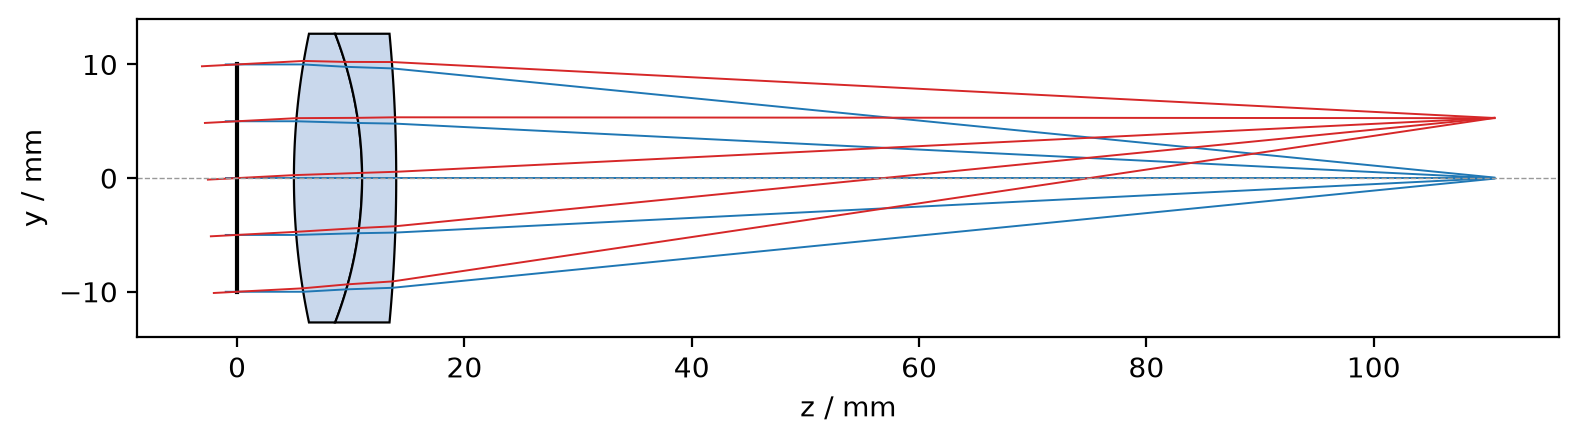
\includegraphics[width=\linewidth]{abbildungen/layout.png}
  \caption{Linsenschnitt des Achromaten mit Strahlen der Felder 0° (blau) und 3° (rot),
    gezeichnet mit \code{rt.layout} und \code{rt.trace.trace(..., record_path=True)}.}
\end{figure}

\begin{longtable}{@{}L{4.4cm}L{10.3cm}@{}}
\toprule
Funktion & Ergebnis \\ \midrule \endhead
\code{surfaces(cs)} & \code{SurfaceLayout} je Fläche: \code{id}, \code{element},
  \code{kind}, \code{rotation} $(3,3)$, \code{translation} (globaler Scheitel), \code{shape},
  \code{curvature}, \code{conic_constant}, \code{coefficients}, \code{max_radius},
  \code{aperture} (\code{None} oder (Typ, Parameter)), \code{medium_front},
  \code{medium_back}, \code{to_global} (4$\times$4) \\
\code{elements(cs)} & \code{CompiledElement}: \code{name}, \code{kind},
  \code{first_surface}, \code{surface_count}, \code{media}, \code{segmented} \\
\code{node_frames(cs)}, \code{reference_frame(cs, ptr)} & Koordinatensysteme aller Knoten
  (\code{location}, \code{reference}, \code{to_global}) \\
\code{sag(cs, fläche, x, y)} & Pfeilhöhe in lokalen Koordinaten; NaN außerhalb des
  Formbereichs \\
\code{normal(cs, fläche, x, y, frame="local")} & Einheitsnormale, \code{"local"} oder
  \code{"global"} \\
\code{profile(cs, fläche, plane="yz", samples=101)} & Polylinien in der Schnittebene,
  global; ein Ring liefert zwei \\
\code{outlines(cs, element, plane="yz", samples=101)} & geschlossene Umrisse der
  Glassegmente von Linsen und segmentierten Platten \\
\bottomrule
\end{longtable}
Schnittebenen sind \code{"yz"}, \code{"xz"} oder \code{(punkt, normale)}; Profile gibt es nur
für Ebenen parallel zur lokalen $z$-Achse der Fläche. Platten aus einem Material, Spiegel und
dünne Elemente haben keine Umrisse; man zeichnet ihre Profile.

% -----------------------------------------------------------------------------
\chapter{Berichte, Ergebnisformat und Plots}
\label{chap:berichte}

\section{Berichte}

\begin{itemize}
  \item \code{dimension_report(cs)} -- Mittendicke, Randdicke, Durchmesser und
        Halbdurchmesser je Glassegment (\code{DimensionReport.segments});
  \item \code{system_report(cs, path, wavelength)} -- Systemeinstellungen und paraxiale
        Prescription (\code{SystemReport}); ist der Pfad nicht paraxial auswertbar, ist
        \code{prescription} \code{None} mit Warnung \code{report.paraxial_unavailable};
  \item \code{raytrace_report(cs, path, *, start)} -- je Strahl und Slot globale und lokale
        Koordinaten, Richtung, OPL, Gewicht und Status (\code{RaytraceReport.rows}).
\end{itemize}
Jeder Bericht hat \code{to_csv()} (auch \code{rt.reports.to_csv(bericht)}): kommagetrennt,
Kopfzeile, Gleitkommazahlen in der kürzesten Darstellung, die bitgleich zurückgelesen wird, NaN
und \code{None} als leeres Feld, Status als Name.

\section{Ergebnisformat \code{raytatouille-result}}

Jedes Ergebnisobjekt hat \code{to_dict()} (reine Python-Werte und NumPy-Arrays) und
\code{to_json(indent=None)}. \code{rt.results.load_json(text)} liest den Text zurück
(\code{Result} mit \code{type}, \code{schema_version}, \code{data}); der Roundtrip ist
bitgleich für die \emph{Daten} (nicht die Objekte). Arrays stehen als
\code{{"dtype": …, "shape": …, "values": …}}, NaN als Zeichenkette. Das Format eignet sich, um
Ergebnisse zwischen Prozessen auszutauschen -- etwa zwischen einem Rechendienst und einer
Oberfläche --, oder um Referenzergebnisse für Regressionstests abzulegen.

\begin{pycode}[title={\code{ex16_berichte.py}}]
"""Berichte als CSV, Ergebnisse als JSON und die eingebauten Plots."""
import csv
import io
import sys
from pathlib import Path

import matplotlib
matplotlib.use("Agg")
import matplotlib.pyplot as plt
import raytatouille as rt
from raytatouille import analysis as an
from achromat import achromat_system, bibliothek

cs = rt.compile(achromat_system(), bibliothek())

dims = an.dimension_report(cs)
print(dims.to_csv())
sysrep = an.system_report(cs, "main")
print("\n".join(sysrep.to_csv().splitlines()[:8]))
start = rt.trace.make_rays(cs, rt.trace.FanYPupil(n=3), fields=[2])
tr = an.raytrace_report(cs, "main", start=start)
print(f"Raytrace-Bericht: {tr.rays} Strahlen × {tr.slots} Slots")
for zeile in list(csv.DictReader(io.StringIO(tr.to_csv())))[:6]:     # ausgewählte Spalten
    print({k: zeile[k] for k in ("ray", "slot", "surface", "y", "z", "opl", "status")})

spot = an.spot(cs, field=2, rays="hexapolar:8")
text = spot.to_json()
r = rt.results.load_json(text)
print("Ergebnisformat:", r.type, r.schema_version, "| Schlüssel:", list(r.data)[:6])
print("bitgleich:", r.data["x"].tobytes() == spot.x.tobytes())

ziel = Path(sys.argv[1]) if len(sys.argv) > 1 else Path(".")
fig, axes = plt.subplots(2, 2, figsize=(10, 8))
rt.plot.spot(spot, axes[0, 0])
rt.plot.ray_fan(an.ray_fan(cs, field=2), axes[0, 1])
rt.plot.opd_map(an.opd_map(cs, field=0, grid=33), axes[1, 0])
rt.plot.field_curvature(an.field_curvature(cs, samples=9), axes[1, 1])
fig.tight_layout()
fig.savefig(ziel / "plots_geometrisch.png", dpi=150)
fig, axes = plt.subplots(1, 2, figsize=(10, 4))
s10 = rt.apply_patch(achromat_system(), [{"op": "replace", "path": "/aperture/value", "value": 10.0},
    {"op": "replace", "path": "/root/children/0/surfaces/0/aperture/radius", "value": 5.0}])
cs10 = rt.compile(s10, bibliothek())
rt.plot.mtf(an.mtf(cs10, field=0), axes[0])
rt.plot.psf(an.psf(cs10, field=0, wavelengths=[1], padding=8), axes[1])
axes[1].set_xlim(-15, 15); axes[1].set_ylim(-15, 15)
fig.tight_layout()
fig.savefig(ziel / "plots_beugung.png", dpi=150)
\end{pycode}
\begin{ausgabe}
element,first_surface,coaxial,centre_thickness,semi_diameter_first,semi_diameter_second,aperture_first,aperture_second,edge_thickness,diameter,active
1,1,true,6.0,12.7,12.7,CIRCULAR,CIRCULAR,2.3035161094185685,25.4,true
1,2,true,3.0,12.7,12.7,CIRCULAR,CIRCULAR,4.780544551866507,25.4,true

key,value
path,0
wavelength,1
wavelengths_um[0],0.4861
wavelengths_um[1],0.5876
wavelengths_um[2],0.6563
reference_wavelength,1
field_count,3
Raytrace-Bericht: 3 Strahlen × 6 Slots
{'ray': '0', 'slot': '0', 'surface': '', 'y': '-10.107188825600307', 'z': '-2.0452846326765344', 'opl': '0.0', 'status': 'ALIVE'}
{'ray': '0', 'slot': '1', 'surface': '0', 'y': '-10.0', 'z': '0.0', 'opl': '2.048649438239961', 'status': 'ALIVE'}
{'ray': '0', 'slot': '2', 'surface': '1', 'y': '-9.697638571056052', 'z': '5.769399754776292', 'opl': '7.827540736678369', 'status': 'ALIVE'}
{'ray': '0', 'slot': '3', 'surface': '2', 'y': '-9.345426510658275', 'z': '9.736750040831627', 'opl': '13.870551478840959', 'status': 'ALIVE'}
{'ray': '0', 'slot': '4', 'surface': '3', 'y': '-9.088142950175145', 'z': '13.698007517376261', 'opl': '20.303263079100336', 'status': 'ALIVE'}
{'ray': '0', 'slot': '5', 'surface': '4', 'y': '5.289730175124824', 'z': '110.614', 'opl': '118.30665051306643', 'status': 'ALIVE'}
Ergebnisformat: SpotDiagram 0.1.23 | Schlüssel: ['field', 'wavelength', 'image_surface', 'chief', 'stats', 'rays_launched']
bitgleich: True
\end{ausgabe}

\section{Plots}

\code{rt.plot} zeichnet Ergebnisse mit matplotlib (optional, \code{pip install
raytatouille[plot]}; Import erst beim Aufruf). Jede Funktion zeichnet in \code{ax} (\code{None}:
neue Abbildung) und gibt die Achsen zurück: \code{spot}, \code{ray_fan}, \code{opd_map},
\code{opd_fan}, \code{distortion}, \code{field_curvature}, \code{longitudinal_colour},
\code{psf} (\code{log=True}, \code{floor}), \code{mtf}, \code{encircled_energy},
\code{through_focus}. Nicht angekommene Strahlen werden ausgelassen. Für Berichte in einer
eigenen Anwendung sind diese Funktionen ein Ausgangspunkt; die Beschriftungen sind englisch und
lassen sich über die zurückgegebenen Achsen ändern.

\begin{figure}[htbp]
  \centering
  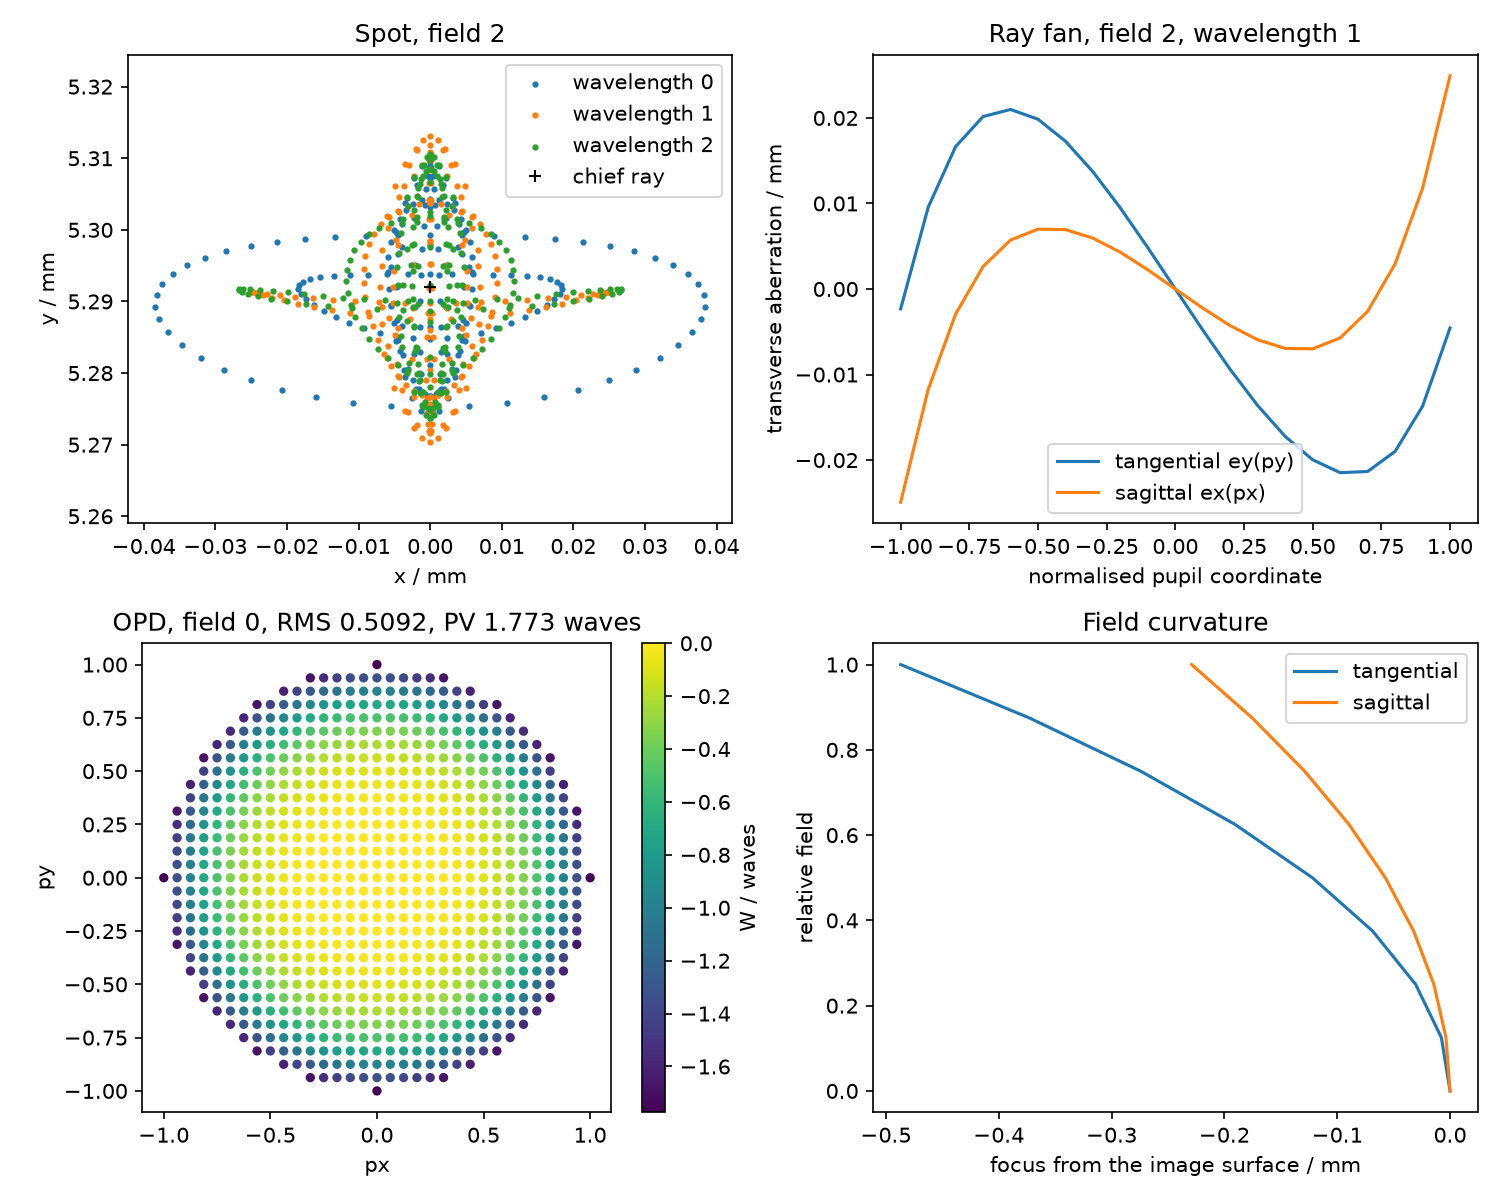
\includegraphics[width=0.95\linewidth]{abbildungen/plots_geometrisch.png}
  \caption{\code{rt.plot.spot}, \code{ray_fan}, \code{opd_map} und \code{field_curvature} für
    den Achromaten.}
\end{figure}
\begin{figure}[htbp]
  \centering
  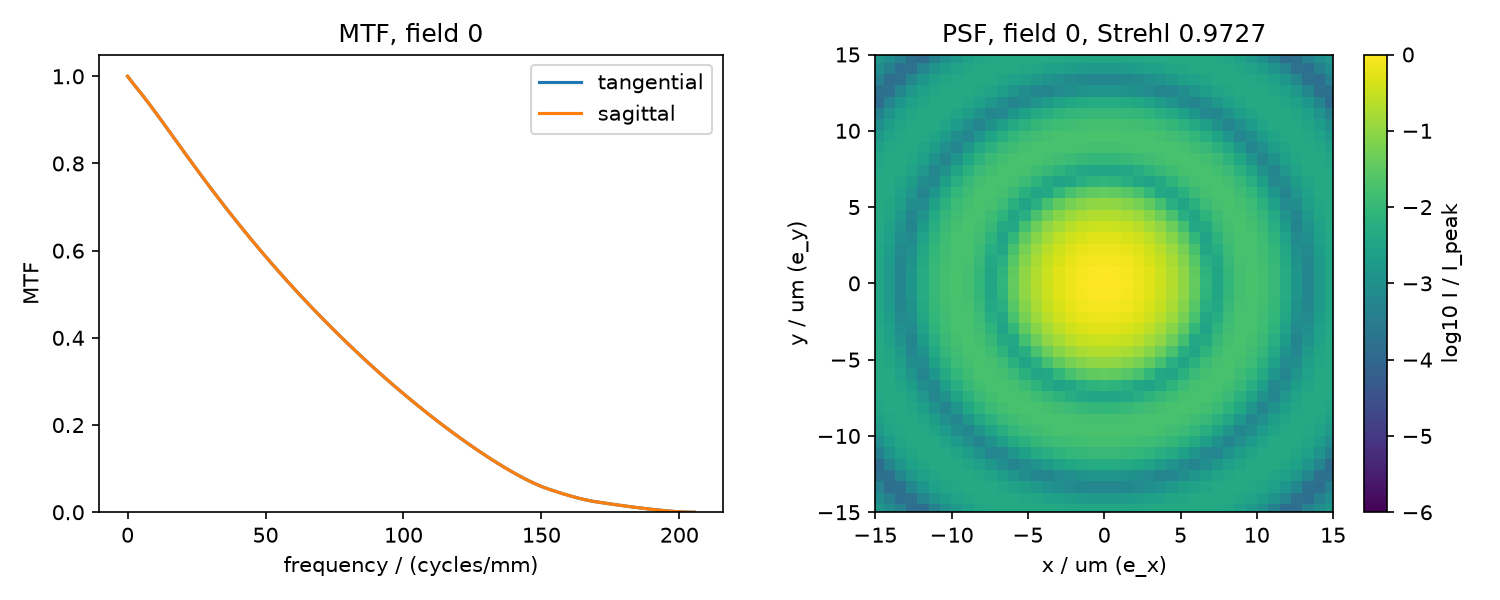
\includegraphics[width=0.95\linewidth]{abbildungen/plots_beugung.png}
  \caption{\code{rt.plot.mtf} und \code{rt.plot.psf} (logarithmisch) des auf F/10 abgeblendeten
    Achromaten.}
\end{figure}

\section{JSON-Schemas der Dateiformate}
\label{sec:schemas}

Das Paket liefert die JSON-Schemas (Draft 2020-12) seiner Dateiformate mit:
\code{rt.schema("system")} für \code{.rtt.json}, \code{rt.schema("result")} für das
Ergebnisformat und \code{rt.schema("coatings")} für Coating-Kataloge, jeweils als \code{dict}.
Damit lassen sich Dateien in eigenen Werkzeugen prüfen oder Editoren mit Vervollständigung
versorgen, ohne das Repository zu kennen. Die Schemas prüfen Aufbau und Typen; die vollständige
Prüfung mit Querbezügen (Namen, Pfade, Wertebereiche) bleibt \code{rt.validate}.

% =============================================================================
\part{Einbindung in eigene Programme}
% =============================================================================

\chapter{Nebenläufigkeit, Fortschritt und Abbruch}
\label{chap:nebenlaeufig}

\section{Threads in der Bibliothek}

Raytatouille rechnet selbst parallel (oneTBB). Der Parameter \code{threads} begrenzt die Zahl
der Arbeits-Threads einer Rechnung; \code{None} nutzt alle Kerne, \code{threads < 1} ist ein
\code{ValueError}. Das Ergebnis ist für jede Threadzahl bitgleich -- Tests müssen also keine
Toleranzen für Parallelität vorsehen.

\section{Python-Threads und die GIL}

Während einer Rechnung gibt die Bibliothek die GIL frei. Mehrere Python-Threads können deshalb
gleichzeitig rechnen, und eine Oberfläche bleibt bedienbar, wenn die Rechnung in einem
Hintergrund-Thread läuft. Regeln:
\begin{itemize}
  \item Ein \code{CompiledSystem} ist unveränderlich und darf von beliebig vielen Threads
        gleichzeitig benutzt werden.
  \item Einen \code{RayBatch} nicht lesen oder ändern, während \code{trace} oder
        \code{make_rays} darauf läuft, und nicht zwei \code{trace}-Aufrufe auf demselben Batch
        starten. Dasselbe gilt für einen \code{RayBatch}, der als \code{start} an eine Analyse
        geht.
  \item \code{MaterialLibrary} und \code{CoatingLibrary} während laufender Rechnungen nicht
        erweitern.
  \item Wer mehrere Rechnungen parallel in Python-Threads startet, setzt \code{threads=1} (oder
        einen kleinen Wert) je Rechnung, damit sich die Thread-Pools nicht gegenseitig
        überbuchen.
  \item \code{System} und \code{Editor} sind gewöhnliche Python-Objekte ohne eigene
        Synchronisation; Änderungen aus mehreren Threads muss die Anwendung selbst schützen.
\end{itemize}

\section{Fortschritt und Abbruch}

Lange Läufe -- \code{make_rays}, \code{trace}, die Bündel- und Sweep-Analysen und
\code{optimize} -- nehmen zwei Argumente an:
\begin{description}
  \item[\code{progress(done, total, stage)}] wird mit gehaltener GIL aus irgendeinem Thread
        gerufen, höchstens alle \SI{50}{ms} und zuletzt mit \code{done == total}. Stufen sind
        \code{"aim"} und \code{"trace"} je Strahlbündel, \code{"field"} bei Sweeps,
        \code{"wavelength"} bei den Farbanalysen, \code{"jacobian"} und \code{"optimize"} bei der
        Optimierung. Eine Ausnahme im Callback beendet die Rechnung und wird weitergereicht.
        Der Callback darf \emph{keine} Raytatouille-Rechnung starten.
  \item[\code{cancel=rt.CancelToken()}] \code{token.cancel()} aus einem anderen Thread beendet
        die Rechnung nach höchstens einem Block je Arbeits-Thread mit \code{rt.Cancelled}
        (Ausgaben dann undefiniert). Ausnahme: \code{optimize} endet mit Status
        \code{CANCELLED} und dem letzten akzeptierten Stand.
\end{description}
Die Einzelpunktfunktionen (\code{*_at}) und \code{seidel} haben beides nicht; sie sind schnell.
Weder \code{progress} noch \code{cancel} ändern ein Ergebnis.

\begin{pycode}[title={\code{ex17_nebenlaeufigkeit.py}}]
"""Lange Rechnungen: Fortschritt, Abbruch, Threads und parallele Auswertung."""
import threading
import time
from concurrent.futures import ThreadPoolExecutor

import numpy as np
import raytatouille as rt
from rtt_bausteine import singlet

cs = rt.compile(singlet())

# 1. Fortschritt: progress(done, total, stage), höchstens alle 50 ms, zuletzt done == total.
#    Wie viele Meldungen dazwischen kommen, hängt von Zeit und Threads ab; sicher ist die letzte.
meldungen = []
rt.analysis.spot(cs, field=2, rays="hexapolar:40",
                 progress=lambda done, total, stage: meldungen.append((stage, done, total)))
print("letzte Meldung:", meldungen[-1], "| mindestens eine:", len(meldungen) >= 1)

# 2. Abbruch aus einem anderen Thread (z. B. ein GUI-Knopf)
token = rt.CancelToken()
ergebnis = []

def arbeit():
    try:
        rt.analysis.spot(cs, field=2, rays="hexapolar:400", cancel=token)
        ergebnis.append("fertig")
    except rt.Cancelled:
        ergebnis.append("abgebrochen")

t = threading.Thread(target=arbeit)
t.start()
time.sleep(0.05)
token.cancel()
t.join()
print("Lauf:", ergebnis[0], "| token.cancelled:", token.cancelled)

# 3. Ergebnisse sind bitgleich für jede Threadzahl
a = rt.analysis.spot(cs, field=2, rays="hexapolar:20", threads=1)
b = rt.analysis.spot(cs, field=2, rays="hexapolar:20")
print("threads=1 und alle Threads bitgleich:", a.x.tobytes() == b.x.tobytes())

# 4. Mehrere Analysen parallel: die GIL ist während der Rechnung freigegeben
def rms(feld):
    return rt.analysis.spot(cs, field=feld, rays="hexapolar:20", threads=1).stats.rms_centroid

with ThreadPoolExecutor(max_workers=3) as pool:
    werte = list(pool.map(rms, range(cs.field_count)))
print("RMS je Feld (µm):", np.round(np.array(werte) * 1e3, 2).tolist())
\end{pycode}
\begin{ausgabe}
letzte Meldung: ('trace', 4921, 4921) | mindestens eine: True
Lauf: abgebrochen | token.cancelled: True
threads=1 und alle Threads bitgleich: True
RMS je Feld (µm): [59.87, 97.44, 138.15]
\end{ausgabe}

\section{Muster für eine grafische Oberfläche}

\begin{pycode}
import threading
import raytatouille as rt

class SpotAuftrag:
    """Startet eine Spotrechnung im Hintergrund; die GUI fragt den Zustand ab."""

    def __init__(self, cs: rt.CompiledSystem, feld: int):
        self.token = rt.CancelToken()
        self.fortschritt = 0.0
        self.ergebnis = None
        self.fehler = None
        self._t = threading.Thread(target=self._lauf, args=(cs, feld), daemon=True)
        self._t.start()

    def _melde(self, done, total, stage):
        self.fortschritt = done / total if total else 1.0   # nur Zustand setzen, nicht rechnen

    def _lauf(self, cs, feld):
        try:
            self.ergebnis = rt.analysis.spot(cs, field=feld, rays="hexapolar:30",
                                             cancel=self.token, progress=self._melde)
        except rt.Cancelled:
            self.fehler = "abgebrochen"
        except rt.RaytatouilleError as e:
            self.fehler = str(e)

    def abbrechen(self):            # vom "Abbrechen"-Knopf
        self.token.cancel()
\end{pycode}
In Qt oder Tk übergibt man den Fortschritt per Signal bzw. \code{after()} an den
GUI-Thread; der Callback selbst sollte nur Zustand setzen.

\section{Prozesse statt Threads}
\label{sec:prozesse}

Für sehr viele unabhängige Rechnungen (Monte Carlo, große Sweeps) lohnt
\code{concurrent.futures.ProcessPoolExecutor}. Seit 0.10 lässt sich ein \code{System} picklen;
es reist dabei als kanonische Dateiform, \code{copy.copy} und \code{copy.deepcopy} gehen
denselben Weg. \code{CompiledSystem} und Ergebnisobjekte bleiben ohne Pickle: Ergebnisse gibt
man als einfache Zahlen oder als \code{to_json()} zurück, und Kataloge lädt jeder Prozess einmal
in einer Initialisierungsfunktion. Das Beispiel zeigt dazu die JSON-Schemas des Pakets
(Abschnitt~\ref{sec:schemas}):
\begin{pycode}[title={\code{ex24_prozesse_schemas.py}}]
"""System in andere Prozesse schicken (pickle) und die JSON-Schemas des Pakets nutzen."""
import pickle
from concurrent.futures import ProcessPoolExecutor

import raytatouille as rt
from rtt_bausteine import singlet


def efl(system: rt.System) -> float:
    return rt.paraxial.first_order(system).efl      # nimmt auch ein System (kompiliert selbst)


if __name__ == "__main__":
    s = singlet()
    kopie = pickle.loads(pickle.dumps(s))
    print("pickle über die kanonische Dateiform:", kopie.to_json() == s.to_json())
    varianten = [singlet(r1=r) for r in (50.0, 51.68, 53.0)]
    with ProcessPoolExecutor(max_workers=3) as pool:
        print("EFL je Prozess:", [f"{f:.3f}" for f in pool.map(efl, varianten)])

    schema = rt.schema("system")                     # auch "result" und "coatings"
    print("Schema:", schema["$schema"], "| Titel:", schema.get("title"))
    print("Pflichtschlüssel:", schema["required"])
\end{pycode}
\begin{ausgabe}
pickle über die kanonische Dateiform: True
EFL je Prozess: ['96.800', '100.053', '102.608']
Schema: https://json-schema.org/draft/2020-12/schema | Titel: Raytatouille system file (.rtt.json), schema 0.11
Pflichtschlüssel: ['schema_version', 'units', 'wavelengths', 'aperture', 'fields', 'root', 'paths']
\end{ausgabe}
\code{ProcessPoolExecutor} startet neue Interpreter (Windows, macOS und ab Python~3.14 auch
Linux, Startmethode \code{forkserver}); der Schutz \code{if __name__ == "__main__":} ist deshalb
Pflicht.

% -----------------------------------------------------------------------------
\chapter{Muster für eigene Anwendungen}
\label{chap:muster}

\section{Eine Studie als wiederverwendbare Klasse}

Das folgende Beispiel kapselt eine Biegungsstudie: Für eine feste Brennweite wird die Form
eines Singlets über den Coddington-Formfaktor $q=(R_2+R_1)/(R_2-R_1)$ variiert. Je Form wird
der Detektor in den paraxialen Fokus gelegt und der RMS-Spot sowie die Strehl-Zahl berechnet.
Fehlgeschlagene Punkte werden protokolliert statt das Programm abzubrechen; die Ergebnisse
gehen als Datenklassen in eine CSV-Datei.

\begin{pycode}[title={\code{ex18_anwendung.py}}]
"""Einbindung in eine eigene Anwendung: eine Biegungsstudie als wiederverwendbare Klasse."""
from __future__ import annotations

import csv
import io
import warnings
from dataclasses import asdict, dataclass

import numpy as np
import raytatouille as rt
from rtt_bausteine import als_system, blende, detektor, linse, system


@dataclass(frozen=True)
class Messpunkt:
    biegung: float          # Coddington-Formfaktor q = (R2 + R1) / (R2 - R1)
    r1: float
    r2: float
    efl: float
    rms_um: float
    strehl: float
    verloren: int


class Biegungsstudie:
    """Variiert die Biegung eines Singlets bei fester Brennweite und bewertet jede Form."""

    def __init__(self, f: float = 100.0, n: float = 1.5168, dicke: float = 4.0, epd: float = 10.0):
        self.f, self.n, self.dicke, self.epd = f, n, dicke, epd

    def radien(self, q: float) -> tuple[float, float]:
        # dünne Linse: 1/f = (n-1)(1/R1 - 1/R2), q = (R2+R1)/(R2-R1)
        c = 1.0 / ((self.n - 1.0) * self.f)          # c1 - c2
        c1, c2 = c * (q + 1.0) / 2.0, c * (q - 1.0) / 2.0
        return (1.0 / c1 if c1 else None), (1.0 / c2 if c2 else None)

    def system(self, q: float, z_bild: float | None = None) -> rt.System:
        r1, r2 = self.radien(q)
        return als_system(system(
            f"Singlet q={q:+.2f}",
            [blende(0.0, self.epd / 2),
             linse("L1", 2.0, [r1, r2], [self.dicke], f"CONST:{self.n}", 12.7),
             detektor(z_bild if z_bild is not None else self.f + self.dicke)],
            epd=self.epd, wellenlaengen=[{"um": 0.5876, "reference": True}]))

    def bewerte(self, q: float) -> Messpunkt:
        # 1. paraxiale Bildlage bestimmen, 2. Detektor dorthin legen und auswerten
        fo = rt.paraxial.first_order(rt.compile(self.system(q)))
        cs = rt.compile(self.system(q, fo.image_z))
        spot = rt.analysis.spot(cs, wavelength=0, rays="hexapolar:10")
        with warnings.catch_warnings():
            warnings.simplefilter("ignore", rt.RaytatouilleWarning)
            fit = rt.analysis.zernike_fit(rt.analysis.pupil_function(cs, grid=48))
        r1, r2 = self.radien(q)
        return Messpunkt(q, r1 or float("inf"), r2 or float("inf"), fo.efl,
                         spot.stats.rms_centroid * 1e3, fit.strehl,
                         spot.rays_launched - spot.rays_arrived)

    def lauf(self, werte) -> list[Messpunkt]:
        punkte = []
        for q in werte:
            try:
                punkte.append(self.bewerte(float(q)))
            except (rt.CompileError, rt.AnalysisError) as e:
                print(f"q = {q:+.2f} übersprungen: {e}")
        return punkte


studie = Biegungsstudie()
punkte = studie.lauf(np.linspace(-1.0, 2.0, 7))
for p in punkte:
    print(f"q {p.biegung:+.2f}: R1 {p.r1:9.2f}  R2 {p.r2:9.2f}  EFL {p.efl:7.3f}  "
          f"RMS {p.rms_um:6.2f} µm  Strehl {p.strehl:.3f}")
beste = min(punkte, key=lambda p: p.rms_um)
print(f"beste Biegung im Raster: q = {beste.biegung:+.2f}")

puffer = io.StringIO()
w = csv.DictWriter(puffer, fieldnames=list(asdict(punkte[0])))
w.writeheader()
w.writerows(asdict(p) for p in punkte)
print(puffer.getvalue().splitlines()[0])
\end{pycode}
\begin{ausgabe}
q -1.00: R1       inf  R2    -51.68  EFL 100.053  RMS  31.15 µm  Strehl 0.752
q -0.50: R1    206.72  R2    -68.91  EFL 100.550  RMS  19.03 µm  Strehl 0.900
q +0.00: R1    103.36  R2   -103.36  EFL 100.716  RMS  11.26 µm  Strehl 0.964
q +0.50: R1     68.91  R2   -206.72  EFL 100.550  RMS   7.59 µm  Strehl 0.983
q +1.00: R1     51.68  R2       inf  EFL 100.053  RMS   7.84 µm  Strehl 0.982
q +1.50: R1     41.34  R2    206.72  EFL  99.235  RMS  11.85 µm  Strehl 0.958
q +2.00: R1     34.45  R2    103.36  EFL  98.113  RMS  19.50 µm  Strehl 0.887
beste Biegung im Raster: q = +0.50
biegung,r1,r2,efl,rms_um,strehl,verloren
\end{ausgabe}

Das Minimum liegt wie erwartet bei einer leicht gekrümmten Plankonvexform ($q\approx0{,}5$ bis
$1$; die Theorie der dünnen Linse liefert für $n=1{,}52$ etwa $q\approx0{,}7$).

\section{Empfehlungen}

\begin{description}
  \item[Einmal kompilieren.] \code{rt.compile} ist teurer als eine einzelne Analyse. Kompilierte
        Systeme in einem Cache halten (Schlüssel z.\,B. \code{(system.to_json(),
        konfiguration)}), solange sich Modell und Kataloge nicht ändern.
  \item[Kataloge zentral laden.] Eine \code{MaterialLibrary} pro Anwendung bzw. Prozess, beim
        Start befüllt und danach nur noch gelesen.
  \item[Pointer aus Namen bestimmen.] \code{locate_surface}, \code{locate_node} statt fester
        Indizes; Flächen-IDs sind die stabilen Schlüssel.
  \item[Fehler in Schichten behandeln.] \code{ParseError}/\code{CompileError} sind
        Eingabefehler (dem Benutzer mit Pointer zeigen), \code{AnalysisError} heißt »für diesen
        Punkt kein Ergebnis« (überspringen, protokollieren), \code{ValueError} meist ein
        Programmierfehler. \code{rt.RaytatouilleError} fängt alle Fehler der Bibliothek.
  \item[Warnungen auswerten statt ignorieren.] \code{result.warnings} und
        \code{result.losses} gehören in jedes Protokoll; global abgeschaltete Warnungen
        verbergen echte Probleme (z.\,B. stark vignettierte Bündel).
  \item[Reproduzierbar rechnen.] Zufall nur mit Startwert; Ergebnisse sind bitgleich. Damit
        eignen sich gespeicherte \code{to_json()}-Ergebnisse als Referenz in Regressionstests.
  \item[Typen prüfen.] Das Paket enthält Typ-Stubs (\code{py.typed}); \code{mypy --strict}
        erkennt falsche Argumente und \code{None}-Fälle (z.\,B. \code{fo.entrance_pupil}
        ist \code{Pupil | None}).
  \item[Version festschreiben.] \code{raytatouille==1.0.*} in den Abhängigkeiten; beim Wechsel
        die eigenen Referenzergebnisse neu prüfen.
\end{description}

\section{Tests im eigenen Projekt}

\begin{pycode}
# test_optik.py (pytest)
import warnings
import pytest
import raytatouille as rt
from rtt_bausteine import singlet

@pytest.fixture(scope="module")
def cs():
    return rt.compile(singlet())

def test_brennweite(cs):
    assert rt.paraxial.first_order(cs).efl == pytest.approx(100.0527, abs=1e-4)

def test_keine_unerwarteten_warnungen(cs):
    with warnings.catch_warnings():
        warnings.simplefilter("error", rt.RaytatouilleWarning)
        rt.analysis.spot(cs, field=2)

def test_bitgleich_mit_referenz(cs, tmp_path):
    a = rt.analysis.spot(cs, field=1, rays="hexapolar:4")
    b = rt.results.load_json(a.to_json()).data
    assert b["x"].tobytes() == a.x.tobytes()
\end{pycode}

% -----------------------------------------------------------------------------
\chapter{Fallstudie: eine eigene Toleranzanalyse}
\label{chap:toleranz}

Für die üblichen Fälle gibt es seit 0.9 die eingebaute Toleranzierung
(Kapitel~\ref{chap:toleranzierung}). Eine eigene Analyse lohnt, wenn die Güte etwas ist, das
kein Operand ausdrückt, oder wenn die Störungen nicht in das Schema passen. Mit
\code{apply_patch} und eigenen Startstrahlen lässt sie sich in wenigen Zeilen bauen. Dabei zeigt
sich eine wichtige Eigenschaft der Zielung:

\begin{achtung}[Dezentrierte und gekippte Systeme]
Sobald eine Fläche dezentriert oder gekippt ist, ist der Pfad nicht mehr rotationssymmetrisch.
\code{make_rays} und alle Analysen in der Komfortform (\code{spot}, \code{opd_map},
\code{ray_fan}, \code{pupil_function}, \ldots) lösen dann
\code{ParaxialError: … decentred from the z axis; the path is not rotationally symmetric} aus,
weil die Zielung paraxiale Daten braucht. Der Ausweg: Startstrahlen am \emph{Nominalsystem}
zielen und durch das gestörte System verfolgen -- so wie ein reales Bündel, das von der
Fertigung nichts weiß.
\end{achtung}

\begin{pycode}[title={\code{ex19_monte_carlo.py}}]
"""Eigene Monte-Carlo-Toleranzanalyse mit apply_patch, ohne rt.tolerance."""
import warnings

import numpy as np
import raytatouille as rt
from achromat import achromat_system, bibliothek

lib = bibliothek()
nominal = achromat_system()
l1 = nominal.locate_node("L1")
s1 = nominal.locate_surface("L1.S1")
s3 = nominal.locate_surface("L1.S3")

# Toleranzen: (Pointer in der Bearbeitungsform, Nennwert, Standardabweichung)
toleranzen = [
    (s1 + "/shape/base/radius/value", 61.5, 0.10),
    (s3 + "/shape/base/radius/value", -136.9, 0.30),
    (l1 + "/pose/position/1/value", 0.0, 0.02),      # Dezentrierung y der Linse
    (l1 + "/pose/rotation_deg/0/value", 0.0, 0.05),  # Verkippung um x in Grad
]
for ptr, nenn, _ in toleranzen:
    assert nominal.json_at(ptr) == nenn, (ptr, nominal.json_at(ptr))


# Gekippte oder dezentrierte Systeme sind nicht rotationssymmetrisch: make_rays und die
# Komfortanalysen (spot, opd_map, ...) lehnen sie mit ParaxialError ab. Deshalb werden die
# Startstrahlen einmal am Nominalsystem gezielt und dann durch jedes gestörte System verfolgt.
cs_nominal = rt.compile(nominal, lib)
start = rt.trace.make_rays(cs_nominal, rt.trace.HexapolarPupil(rings=6), fields=[0])


def guete(s: rt.System) -> float:
    """RMS-Spotradius in µm um den Schwerpunkt, Feld 0, Referenzwellenlänge."""
    cs = rt.compile(s, lib)
    rays = rt.trace.RayBatch(len(start))
    for spalte in ("pos_x", "pos_y", "pos_z", "dir_x", "dir_y", "dir_z", "wl", "field",
                   "pupil_x", "pupil_y"):
        getattr(rays, spalte)[:] = getattr(start, spalte)   # frische Kopie der Startstrahlen
    rt.trace.trace(cs, rays)
    ok = rays.status == rt.trace.RayStatus.ALIVE
    x, y = rays.pos_x[ok], rays.pos_y[ok]
    return float(np.sqrt(np.mean((x - x.mean()) ** 2 + (y - y.mean()) ** 2))) * 1e3


rng = np.random.default_rng(seed=1)
nenn = guete(nominal)
werte = []
with warnings.catch_warnings():
    warnings.simplefilter("ignore", rt.RaytatouilleWarning)
    for _ in range(200):
        patch = [{"op": "replace", "path": p, "value": float(n + rng.normal(0.0, sd))}
                 for p, n, sd in toleranzen]
        werte.append(guete(rt.apply_patch(nominal, patch)))
werte = np.array(werte)
print(f"nominal RMS {nenn:.2f} µm; 200 Versuche: Mittel {werte.mean():.2f} µm, "
      f"90-%-Quantil {np.quantile(werte, 0.9):.2f} µm, Maximum {werte.max():.2f} µm")
\end{pycode}
\begin{ausgabe}
nominal RMS 28.63 µm; 200 Versuche: Mittel 28.72 µm, 90-%-Quantil 42.48 µm, Maximum 62.04 µm
\end{ausgabe}

Erweiterungen liegen nahe: weitere Toleranzen (Dicken, Brechzahlen über
\code{CONST:}-Materialien oder Katalogvarianten, Verkippung einzelner Flächen), Kompensatoren
(nach jeder Störung den Detektor mit \code{rt.optim.optimize} nachfokussieren, wenn nur
\code{position/2} variabel ist -- für dezentrierte Systeme braucht die Merit-Funktion dann aber
ebenfalls Zielung, siehe oben), Parallelisierung über Prozesse und eine Auswertung über
Wellenfront statt Spot (\code{rt.analysis.opd_points} braucht dieselbe Zielung; mit
\code{jones_pupil(start=…, chief=…)} gibt es eine Startstrahl-Form mit Phase).

% -----------------------------------------------------------------------------
\chapter{Bekannte Grenzen von Version 1.0}
\label{chap:grenzen}

\begin{itemize}
  \item \textbf{Freiformflächen:} Zernike-Terme nach Noll und im Fringe-Satz, XY-Polynome und
        Grid-Sag (ADR~0051). Terme mit Kippung oder Astigmatismus im Scheitel und Grid-Sag haben
        kein paraxiales Modell und damit keine automatische Zielung; Strahlen startet man dort
        selbst oder zielt im Kommandozeilenwerkzeug mit dem Bezug eines Nennsystems
        (Abschnitt~\ref{sec:freiform}). Ebenso braucht die Optimierung solcher Systeme einen
        eigenen Bezug.
  \item \textbf{Zielung nur für rotationssymmetrische und anamorphe Pfade.} Gekippte,
        dezentrierte und gefaltete Pfade brauchen eigene Startstrahlen
        (Kapitel~\ref{chap:toleranz}); ebenso Pfade mit Axicon oder ungerader Asphäre mit
        $A_1\ne0$. Die eingebaute Toleranzierung zielt gestörte Prüflinge mit den Daten des
        Nennsystems.
  \item \textbf{Anamorphe Pfade:} keine paraxialen Operanden, keine Wellenfront (OPD,
        Wellenfront-Generator), keine Feldkurven, Farbfehler und Geister-Startstrahlen; es laufen
        Strahlen, Spot, Strahl-Operanden und der Spot-Generator.
  \item \textbf{Keine globale Optimierung}; Levenberg-Marquardt findet das nächste lokale
        Minimum.
  \item \textbf{Toleranzierung:} keine Korrelationen zwischen Toleranzen, Flächenfehler nur als
        Zernike-Terme, Strehl und MTF nicht als Kriterien, keine Materialtoleranz für Kristalle
        und Metalle.
  \item \textbf{Nur sequenzielles Raytracing} über definierte Pfade; kein nicht-sequenzielles
        Tracing und keine Streuung.
  \item \textbf{Beugung skalar} (Fraunhofer, inkohärent); Pfade mit Kristallmoden haben keine
        Pupillenfunktion, PSF oder Jones-Pupille.
  \item \textbf{Geisterbilder} nur als Zweifachreflexionen, nicht für Basispfade mit
        Beugungsordnungen oder Kristallmoden.
  \item \textbf{ZMX-Import und -Export} nur im Kommandozeilenwerkzeug und in C++, nicht aus
        Python (Anhang~\ref{chap:cli}); Gläser kommen aus AGF-Katalogen. Zernike-Sag- und
        Extended-Polynomial-Flächen einer ZMX-Datei werden noch nicht importiert
        (\code{zmx.surface_unsupported}); Fringe-Zernike und Grid-Sag ebenso nicht. Der Export
        lehnt Freiformterme (\code{export.surface_unsupported}) und Polygon-Aperturen
        (\code{export.aperture_unsupported}) ab.
  \item \textbf{Pickle} nur für \code{System}; \code{CompiledSystem} und Ergebnisse werden
        über JSON ausgetauscht.
  \item Das Ergebnisformat ist innerhalb von 0.1.x verträglich; seine Version zählt getrennt von
        der Paketversion.
\end{itemize}

% =============================================================================
\part{Referenz}
% =============================================================================

\chapter{Funktionsreferenz}
\label{chap:api}

Die Signaturen in diesem Kapitel sind automatisch aus der installierten Version 1.0.0 erzeugt
(Typannotationen der Python-Module bzw. der Typ-Stubs der Erweiterung). \code{SystemLike}
steht für \code{System | CompiledSystem}, \code{PupilSampling} für eine der
Abtastungsklassen aus \code{rt.trace}. Parameter nach \code{*} sind nur als Schlüsselwort
erlaubt. Die Kurzbeschreibungen fassen die Docstrings zusammen; die vollständigen englischen
Docstrings zeigt \code{help(rt.analysis.spot)} usw.

\section{\code{raytatouille}}
\begin{signatur}
load(file: str | os.PathLike) -> System
save(system: System, file: str | os.PathLike) -> None
validate(system: System) -> list[Diagnostic]
compile(
    system: System,
    materials: MaterialLibrary | None = None,
    coatings: CoatingLibrary | None = None,
    *,
    configuration: int | str = 0
) -> CompiledSystem
compile_with_ghosts(
    system: System,
    base: int | str = 0,
    materials: MaterialLibrary | None = None,
    coatings: CoatingLibrary | None = None,
    *,
    max_paths: int = 10000,
    configuration: int | str = 0
) -> GhostSystem
ghost_paths(
    system: CompiledSystem,
    base: int | str = 0,
    *,
    max_paths: int = 10000
) -> list[Path]
apply_patch(system: System, patch: Patch, *, check: Check = 'no_new_errors') -> System
apply_patch_with_inverse(
    system: System,
    patch: Patch,
    *,
    check: Check = 'no_new_errors'
) -> PatchResult
schema(name: str = 'system') -> dict[str, Any]
llm_reference() -> str
\end{signatur}
\begin{longtable}{@{}L{4.2cm}L{10.5cm}@{}}
\toprule
Funktion & Kurzbeschreibung \\ \midrule \endhead
\code{load} & Systemdatei lesen (Migration älterer Schemata); \code{ParseError},
  \code{OSError} \\
\code{save} & kanonischen Text schreiben; \code{OSError} \\
\code{validate} & alle semantischen Prüfungen; Liste von \code{Diagnostic}, wirft nie \\
\code{compile} & \code{CompiledSystem} für eine Konfiguration; \code{CompileError} \\
\code{compile_with_ghosts} & wie \code{compile}, zusätzlich alle Zweifachreflexionen eines
  Pfads; \code{GhostSystem} \\
\code{ghost_paths} & nur die Geisterpfade als \code{model.Path} \\
\code{apply_patch} & Patch anwenden, neues System; \code{EditError} \\
\code{apply_patch_with_inverse} & dazu inverser Patch und Diagnosen (\code{PatchResult}) \\
\code{schema} & JSON-Schema eines Dateiformats (\code{"system"}, \code{"result"},
  \code{"coatings"}, \code{"lenses"}) als \code{dict} \\
\code{llm_reference} & kompakte Befehlsreferenz für Sprachmodelle und Agenten (Markdown,
  englisch) als Text \\
\bottomrule
\end{longtable}
Klassen auf oberster Ebene: \code{System}, \code{CompiledSystem}, \code{CompiledMedium},
\code{Environment}, \code{Field}, \code{Wavelength}, \code{Diagnostic}, \code{Severity},
\code{LoadWarning}, \code{MaterialLibrary}, \code{CoatingLibrary}, \code{GhostSystem},
\code{GhostPaths}, \code{Editor}, \code{PatchResult}, \code{CancelToken} und die Ausnahmen
(Abschnitt~\ref{sec:ausnahmen}).

\section{\code{rt.paraxial}}
\begin{signatur}
first_order(
    system: SystemLike,
    path: int | str = 0,
    wavelength: int | None = None,
    *,
    materials: MaterialLibrary | None = None
) -> FirstOrder
prescription(
    system: SystemLike,
    path: int | str = 0,
    wavelength: int | None = None,
    *,
    materials: MaterialLibrary | None = None
) -> Prescription
seidel(
    system: SystemLike,
    path: int | str = 0,
    wavelength: int | None = None,
    *,
    pair: ChromaticPair | tuple[int, int] | None = None,
    materials: MaterialLibrary | None = None
) -> Seidel
first_order_section(
    system: SystemLike,
    section: Section,
    path: int | str = 0,
    wavelength: int | None = None,
    *,
    materials: MaterialLibrary | None = None
) -> FirstOrder
is_anamorphic(system: CompiledSystem, path: int | str = 0) -> bool
trace_ray_section(
    system: CompiledSystem,
    section: Section,
    z0: float,
    h0: float,
    u0: float,
    path: int | str = 0,
    wavelength: int | None = None
) -> list[RayAtEvent]
\end{signatur}
Alle Funktionen außer \code{is_anamorphic} und \code{trace_ray_section} nehmen auch ein
\code{System} (mit \code{materials}). \code{first_order_section} gibt die erste Ordnung eines
Schnitts (\code{Section.X}, \code{Section.Y}) für anamorphe Pfade, \code{trace_ray_section}
verfolgt einen paraxialen Strahl in einem Schnitt (Liste von \code{RayAtEvent}).
Fehler: \code{ParaxialError}, \code{NoStopError} (Seidel ohne Blende).

\section{\code{rt.trace}}
\begin{signatur}
make_rays(
    system: CompiledSystem,
    sampling: PupilSampling,
    *,
    path: int | str = 0,
    fields: Sequence[int] | None = None,
    wavelength: int | None = None,
    aiming: Aiming = Aiming.REAL,
    threads: int | None = None,
    cancel: CancelToken | None = None,
    progress: Callable | None = None
) -> RayBatch
trace(
    system: CompiledSystem,
    rays: RayBatch,
    *,
    path: int | str = 0,
    threads: int | None = None,
    record_path: bool = False,
    record_rays: npt.ArrayLike | None = None,
    max_recorded_rays: int = 10000,
    polarization: bool = False,
    cancel: CancelToken | None = None,
    progress: ProgressCallback | None = None
) -> TraceStats | tuple[TraceStats, RayPaths]
gauss_pupil_weights(gauss: GaussPupil) -> list[float]
\end{signatur}
Klassen: \code{RayBatch}, \code{RayPaths}, \code{TraceStats}, \code{RayStatus},
\code{Aiming}, \code{CancelToken}, die Abtastungen \code{SinglePupilPoint},
\code{HexapolarPupil}, \code{GridPupil}, \code{FanXPupil}, \code{FanYPupil},
\code{RandomPupil}, \code{GaussPupil}, \code{PointListPupil}; Konstanten
\code{NO_SURFACE} und \code{DEFAULT_MAX_RECORDED_RAYS} (10000); Typalias
\code{ProgressCallback}.

\section{\code{rt.analysis}}
\begin{signatur}
spot(
    system: SystemLike,
    path: int | str = 0,
    field: int = 0,
    wavelength: int | None = None,
    *,
    rays: str | PupilSampling = 'hexapolar:6',
    aiming: Aiming = Aiming.REAL,
    materials: MaterialLibrary | None = None,
    threads: int | None = None,
    lost_warning_fraction: float = 0.5,
    cancel: CancelToken | None = None,
    progress: ProgressCallback | None = None
) -> SpotDiagram
ray_fan(
    system: SystemLike,
    path: int | str = 0,
    field: int = 0,
    wavelength: int | None = None,
    *,
    points: int = 21,
    aiming: Aiming = Aiming.REAL,
    materials: MaterialLibrary | None = None,
    threads: int | None = None,
    lost_warning_fraction: float = 0.5,
    cancel: CancelToken | None = None,
    progress: ProgressCallback | None = None
) -> RayFan
opd_map(
    system: SystemLike,
    path: int | str = 0,
    field: int = 0,
    wavelength: int | None = None,
    *,
    grid: int = 33,
    aiming: Aiming = Aiming.REAL,
    focus_shift: float = 0.0,
    materials: MaterialLibrary | None = None,
    threads: int | None = None,
    lost_warning_fraction: float = 0.5,
    cancel: CancelToken | None = None,
    progress: ProgressCallback | None = None
) -> OpdMap
opd_fan(
    system: SystemLike,
    path: int | str = 0,
    field: int = 0,
    wavelength: int | None = None,
    *,
    points: int = 21,
    aiming: Aiming = Aiming.REAL,
    focus_shift: float = 0.0,
    materials: MaterialLibrary | None = None,
    threads: int | None = None,
    lost_warning_fraction: float = 0.5,
    cancel: CancelToken | None = None,
    progress: ProgressCallback | None = None
) -> OpdFan
opd_points(
    system: SystemLike,
    path: int | str = 0,
    field: int = 0,
    wavelength: int | None = None,
    *,
    rays: str | PupilSampling = 'hexapolar:6',
    aiming: Aiming = Aiming.REAL,
    focus_shift: float = 0.0,
    materials: MaterialLibrary | None = None,
    threads: int | None = None,
    lost_warning_fraction: float = 0.5,
    cancel: CancelToken | None = None,
    progress: ProgressCallback | None = None
) -> OpdPupilPoints
longitudinal_colour(
    system: SystemLike,
    path: int | str = 0,
    *,
    pair: ChromaticPair | tuple[int, int] | None = None,
    zone: float = 1.0,
    aiming: Aiming = Aiming.REAL,
    materials: MaterialLibrary | None = None,
    threads: int | None = None,
    cancel: CancelToken | None = None,
    progress: ProgressCallback | None = None
) -> LongitudinalColour
lateral_colour(
    system: SystemLike,
    path: int | str = 0,
    field: int = 0,
    *,
    aiming: Aiming = Aiming.REAL,
    materials: MaterialLibrary | None = None,
    threads: int | None = None,
    cancel: CancelToken | None = None,
    progress: ProgressCallback | None = None
) -> LateralColour
distortion(
    system: SystemLike,
    path: int | str = 0,
    wavelength: int | None = None,
    *,
    samples: int = 11,
    aiming: Aiming = Aiming.REAL,
    materials: MaterialLibrary | None = None,
    threads: int | None = None,
    cancel: CancelToken | None = None,
    progress: ProgressCallback | None = None
) -> DistortionSweep
distortion_at(
    system: SystemLike,
    field: Field | tuple[float, float],
    path: int | str = 0,
    wavelength: int | None = None,
    *,
    aiming: Aiming = Aiming.REAL,
    materials: MaterialLibrary | None = None,
    threads: int | None = None
) -> DistortionPoint
field_curvature(
    system: SystemLike,
    path: int | str = 0,
    wavelength: int | None = None,
    *,
    samples: int = 11,
    delta: float = 0.001,
    aiming: Aiming = Aiming.REAL,
    materials: MaterialLibrary | None = None,
    threads: int | None = None,
    cancel: CancelToken | None = None,
    progress: ProgressCallback | None = None
) -> FieldCurvatureSweep
field_curvature_at(
    system: SystemLike,
    field: Field | tuple[float, float],
    path: int | str = 0,
    wavelength: int | None = None,
    *,
    delta: float = 0.001,
    aiming: Aiming = Aiming.REAL,
    materials: MaterialLibrary | None = None,
    threads: int | None = None
) -> FieldCurvaturePoint
pupil_cells(grid: int, obscuration: float = 0.0) -> PupilCells
pupil_function(
    system: SystemLike,
    path: int | str = 0,
    field: int = 0,
    wavelength: int | None = None,
    *,
    grid: int = 64,
    apodization: float = 0.0,
    focus_shift: float = 0.0,
    aiming: Aiming = Aiming.REAL,
    with_prt: bool = False,
    materials: MaterialLibrary | None = None,
    threads: int | None = None,
    lost_warning_fraction: float = 0.5,
    mapping_warning: float = 0.01,
    mapping_limit: float = 0.05,
    cancel: CancelToken | None = None,
    progress: ProgressCallback | None = None
) -> PupilFunction
refocus(
    system: SystemLike,
    pupil: PupilFunction,
    focus_shift: float,
    *,
    materials: MaterialLibrary | None = None
) -> PupilFunction
zernike_fit(
    pupil: PupilFunction,
    *,
    terms: int = 37,
    incomplete_warning_fraction: float = 0.01
) -> ZernikeFit
zernike(j: int, rho: float, theta: float) -> float
zernike_radial(n: int, m: int, rho: float) -> float
noll_to_nm(j: int) -> NollIndex
noll_from_nm(n: int, m: int, sine: bool = False) -> int
psf(
    system: SystemLike,
    path: int | str = 0,
    field: int = 0,
    *,
    wavelengths: Sequence[int] | None = None,
    grid: int = 64,
    padding: int = 4,
    apodization: float = 0.0,
    focus_shift: float = 0.0,
    aiming: Aiming = Aiming.REAL,
    aliasing_factor: float = 3.0,
    undersampled_waves: float = 0.5,
    materials: MaterialLibrary | None = None,
    threads: int | None = None,
    lost_warning_fraction: float = 0.5,
    mapping_warning: float = 0.01,
    mapping_limit: float = 0.05,
    cancel: CancelToken | None = None,
    progress: ProgressCallback | None = None
) -> Psf
psf_at(pupil: PupilFunction, points: npt.ArrayLike) -> npt.NDArray[np.float64]
psf_positions(result: Psf) -> npt.NDArray[np.float64]
through_focus(
    system: SystemLike,
    path: int | str = 0,
    field: int = 0,
    wavelength: int | None = None,
    *,
    shifts: Sequence[float],
    grid: int = 64,
    apodization: float = 0.0,
    aiming: Aiming = Aiming.REAL,
    materials: MaterialLibrary | None = None,
    threads: int | None = None,
    lost_warning_fraction: float = 0.5,
    mapping_warning: float = 0.01,
    mapping_limit: float = 0.05,
    cancel: CancelToken | None = None,
    progress: ProgressCallback | None = None
) -> ThroughFocus
mtf(
    system: SystemLike | PupilFunction,
    path: int | str | None = None,
    field: int | None = None,
    *,
    wavelengths: Sequence[int] | None = None,
    grid: int | None = None,
    map: bool = False,
    complex_otf: bool = False,
    apodization: float | None = None,
    focus_shift: float | None = None,
    aiming: Aiming | None = None,
    undersampled_waves: float | None = None,
    materials: MaterialLibrary | None = None,
    threads: int | None = None,
    lost_warning_fraction: float | None = None,
    mapping_warning: float | None = None,
    mapping_limit: float | None = None,
    cancel: CancelToken | None = None,
    progress: ProgressCallback | None = None
) -> Mtf
encircled_energy(
    system: SystemLike | PupilFunction,
    radii: Sequence[float] | int | np.integer[Any],
    path: int | str | None = None,
    field: int | None = None,
    *,
    relative: bool = False,
    centre: EeCentre = EeCentre.REFERENCE,
    wavelengths: Sequence[int] | None = None,
    grid: int | None = None,
    apodization: float | None = None,
    focus_shift: float | None = None,
    aiming: Aiming | None = None,
    undersampled_waves: float | None = None,
    materials: MaterialLibrary | None = None,
    threads: int | None = None,
    lost_warning_fraction: float | None = None,
    mapping_warning: float | None = None,
    mapping_limit: float | None = None,
    cancel: CancelToken | None = None,
    progress: ProgressCallback | None = None
) -> EncircledEnergy
jones_pupil(
    system: SystemLike,
    path: int | str = 0,
    *,
    start: RayBatch | None = None,
    chief: int | None = None,
    field: int | None = None,
    wavelength: int | None = None,
    rays: str | PupilSampling | None = None,
    aiming: Aiming | None = None,
    basis: JonesBasis = JonesBasis.DOUBLE_POLE,
    remove_global_phase: bool = False,
    field_amplitude: bool = False,
    materials: MaterialLibrary | None = None,
    threads: int | None = None,
    lost_warning_fraction: float = 0.5,
    cancel: CancelToken | None = None,
    progress: ProgressCallback | None = None
) -> JonesPupil
stokes_pupil(jones: JonesPupil, e1: complex, e2: complex) -> StokesPupil
path_transmission(
    system: SystemLike,
    path: int | str = 0,
    *,
    start: RayBatch | None = None,
    field: int | None = None,
    wavelength: int | None = None,
    rays: str | PupilSampling | None = None,
    aiming: Aiming | None = None,
    materials: MaterialLibrary | None = None,
    threads: int | None = None,
    lost_warning_fraction: float = 0.5,
    cancel: CancelToken | None = None,
    progress: ProgressCallback | None = None
) -> PathTransmission
opl_difference(
    system: SystemLike,
    path_a: int | str,
    path_b: int | str,
    *,
    start: RayBatch | None = None,
    field: int | None = None,
    wavelength: int | None = None,
    rays: str | PupilSampling | None = None,
    aiming: Aiming | None = None,
    materials: MaterialLibrary | None = None,
    threads: int | None = None,
    lost_warning_fraction: float = 0.5,
    cancel: CancelToken | None = None,
    progress: ProgressCallback | None = None
) -> PathOplDifference
interferogram(
    system: SystemLike,
    path_a: int | str,
    path_b: int | str,
    *,
    start: RayBatch | None = None,
    field: int | None = None,
    wavelength: int | None = None,
    rays: str | PupilSampling | None = None,
    aiming: Aiming | None = None,
    materials: MaterialLibrary | None = None,
    threads: int | None = None,
    lost_warning_fraction: float = 0.5,
    cancel: CancelToken | None = None,
    progress: ProgressCallback | None = None
) -> Interferogram
ghost_ranking(
    ghosts: GhostSystem,
    field: int = 0,
    wavelength: int | None = None,
    *,
    rays: str | PupilSampling = 'hexapolar:6',
    aiming: Aiming = Aiming.REAL,
    resolution_radius: float = 0.005,
    threads: int | None = None,
    lost_warning_fraction: float = 0.5,
    cancel: CancelToken | None = None,
    progress: ProgressCallback | None = None
) -> GhostRanking
raytrace_report(
    system: SystemLike,
    path: int | str = 0,
    *,
    start: RayBatch,
    materials: MaterialLibrary | None = None,
    threads: int | None = None
) -> RaytraceReport
system_report(
    system: SystemLike,
    path: int | str = 0,
    wavelength: int | None = None,
    *,
    materials: MaterialLibrary | None = None
) -> SystemReport
dimension_report(
    system: SystemLike,
    *,
    materials: MaterialLibrary | None = None
) -> DimensionReport
sampling(rays: str | PupilSampling) -> PupilSampling
\end{signatur}

\begin{longtable}{@{}L{4.2cm}L{10.5cm}@{}}
\toprule
Funktion & Kurzbeschreibung \\ \midrule \endhead
\code{spot} & Spotdiagramm eines Felds (\code{wavelength=None}: polychromatisch) \\
\code{ray_fan} & tangentialer und sagittaler Ray Fan \\
\code{opd_map}, \code{opd_fan}, \code{opd_points} & OPD auf Raster, Schnitten oder beliebigen
  Pupillenpunkten \\
\code{longitudinal_colour}, \code{lateral_colour} & Farblängs- und Farbquerfehler \\
\code{distortion}, \code{distortion_at} & Verzeichnung über das Feld bzw. an einem Feldwert \\
\code{field_curvature}, \code{field_curvature_at} & tangentiale und sagittale Bildschale \\
\code{pupil_cells} & Zellen der Pupillenfunktion (Flächenanteil, Abtastpunkt), ohne Trace \\
\code{pupil_function}, \code{refocus} & Pupillenfunktion; Umrechnung auf andere Fokuslage \\
\code{zernike_fit}, \code{zernike}, \code{zernike_radial}, \code{noll_to_nm},
  \code{noll_from_nm} & Zernike-Fit und -Polynome nach Noll \\
\code{psf}, \code{psf_at}, \code{psf_positions} & FFT-PSF, PSF an Punkten, Gitterorte \\
\code{through_focus} & Strehl-Zahl über Fokusverschiebungen \\
\code{mtf}, \code{encircled_energy} & MTF und Encircled Energy (auch aus einer
  \code{PupilFunction}) \\
\code{jones_pupil}, \code{stokes_pupil} & Polarisation in der Pupille \\
\code{path_transmission}, \code{opl_difference}, \code{interferogram} & Pfadanalysen \\
\code{ghost_ranking} & Rangfolge der Geisterbilder \\
\code{raytrace_report}, \code{system_report}, \code{dimension_report} & Berichte \\
\code{sampling} & Kurzform \code{"hexapolar:N"} usw. in eine Abtastung umwandeln \\
\bottomrule
\end{longtable}
Konstanten: \code{MAX_PUPIL_GRID} (2048), \code{MAX_ZERNIKE_TERMS} (231).

\begin{signatur}
irradiance_map(
    system: SystemLike,
    rays: RayPaths | RayBatch,
    *,
    surface: str | None = None,
    path: int | str = 0,
    nx: int = 64,
    ny: int = 64,
    extent: tuple[float, float, float, float] | None = None,
    event: int | None = None,
    wavelength: int | None = None,
    materials: MaterialLibrary | None = None
) -> IrradianceMap
\end{signatur}
\code{irradiance_map} verteilt verfolgte Strahlen (\code{RayBatch} für die Bildfläche oder
\code{RayPaths} für jede Fläche und jedes Ereignis) auf ein Raster in lokalen Koordinaten; Werte
in Gewicht je mm² (\code{IrradianceMap}, Abschnitt~\ref{sec:irradiance}).

\section{\code{rt.polar}}
\begin{signatur}
initial_directions(rays: RayBatch) -> FloatArray
transverse_polarization(rays: RayBatch, polarization: npt.ArrayLike) -> ComplexArray
transmission(rays: RayBatch, polarization: npt.ArrayLike | None = None) -> FloatArray
diattenuation(
    rays: RayBatch | npt.ArrayLike,
    k_in: npt.ArrayLike | None = None,
    k_out: npt.ArrayLike | None = None
) -> Diattenuations | Diattenuation
retardance(
    rays: RayBatch | npt.ArrayLike,
    k: npt.ArrayLike | None = None
) -> Retardances | Retardance
physical_retardance(p: npt.ArrayLike, q: npt.ArrayLike, k_in: npt.ArrayLike) -> Retardance
stokes(
    rays: RayBatch | npt.ArrayLike,
    polarization: npt.ArrayLike,
    axis: npt.ArrayLike,
    /
) -> FloatArray
prt_matrix(
    k_in: npt.ArrayLike,
    k_out: npt.ArrayLike,
    normal: npt.ArrayLike,
    a_s: complex,
    a_p: complex
) -> ComplexArray
geometric_transform(
    k_in: npt.ArrayLike,
    k_out: npt.ArrayLike,
    normal: npt.ArrayLike,
    reflection: bool
) -> FloatArray
\end{signatur}

\section{\code{rt.optim}}
\begin{signatur}
variables(system: System) -> list[Variable]
optimize(
    system: System,
    *,
    materials: MaterialLibrary | None = None,
    coatings: CoatingLibrary | None = None,
    options: OptimizeOptions | None = None,
    threads: int | None = None,
    cancel: CancelToken | None = None,
    progress: ProgressCallback | None = None,
    on_iteration: IterationCallback | None = None
) -> OptimResult
\end{signatur}
Klassen: \code{MeritFunction} (\code{variables}, \code{start()}, \code{size},
\code{generator_sizes}, \code{evaluate(values, threads=None)}), \code{MeritEvaluation},
\code{OptimizeOptions}, \code{OptimResult}, \code{OptimStatus}, \code{OptimIterations},
\code{Variable}, \code{VariableValue}, \code{OperandValue}, \code{GeneratorValue},
\code{GeneratorStats}, \code{IterationState} und der Typ \code{IterationCallback}
(Abschnitt~\ref{sec:on-iteration}); Konstante \code{MERIT_PRECISION} ($10^{-9}$).

\section{\code{rt.tolerance}}
\begin{signatur}
expand(system: System, *, materials: MaterialLibrary | None = None) -> ToleranceItems
sensitivity(
    system: System,
    *,
    materials: MaterialLibrary | None = None,
    coatings: CoatingLibrary | None = None,
    confirm: bool = True,
    compensators: OptimizeOptions | None = None,
    threads: int | None = None,
    cancel: CancelToken | None = None,
    progress: ProgressCallback | None = None
) -> ToleranceSensitivity
monte_carlo(
    system: System,
    *,
    materials: MaterialLibrary | None = None,
    coatings: CoatingLibrary | None = None,
    trials: int | None = None,
    seed: int | None = None,
    percentiles: Sequence[float] = (0.5, 0.9, 0.95, 0.99),
    z: float = 1.959963984540054,
    keep_trials: bool = True,
    compensators: OptimizeOptions | None = None,
    threads: int | None = None,
    cancel: CancelToken | None = None,
    progress: ProgressCallback | None = None
) -> MonteCarloResult
class_limit(
    tolerance_class: ToleranceClass,
    kind: ToleranceKind,
    level: ToleranceLevel
) -> float
abbe_share(tolerance_class: ToleranceClass) -> float
sigma_ratio(distribution: ToleranceDistribution) -> float
\end{signatur}
\begin{longtable}{@{}L{3.2cm}L{11.5cm}@{}}
\toprule
Funktion & Kurzbeschreibung \\ \midrule \endhead
\code{expand} & alle Toleranzen des Satzes mit Herkunft und übersprungenen Zielen
  (\code{ToleranceItems}); \code{CompileError} bei Fehlern im Satz \\
\code{sensitivity} & Einzelstörungen bei $\pm T$ mit Kompensation, RSS und inverse Sensitivität
  je Kriterium (\code{ToleranceSensitivity}) \\
\code{monte_carlo} & Prüflinge mit Seed, Statistik, Perzentile, Ausbeute mit Wilson-Intervall
  (\code{MonteCarloResult}); \code{keep_trials=False} spart die Tabelle der Prüflinge \\
\code{class_limit} & Grenze $T$ einer Klassentoleranz (Klasse, Art, Ebene) \\
\code{abbe_share} & Anteil $p$ von $\nu_d$, der eine Abbe-Klassentoleranz begrenzt \\
\code{sigma_ratio} & $\sigma/T$ einer Verteilung (\code{NORMAL} 0,43981, \code{UNIFORM}
  $1/\sqrt3$, \code{ENDPOINT} 1) \\
\bottomrule
\end{longtable}
\code{cancel} beendet Sensitivität und Monte Carlo mit Status \code{CANCELLED} und den bis dahin
fertigen Ergebnissen, ohne Ausnahme; \code{progress} meldet den Fortschritt.

\section{\code{rt.layout}}
\begin{signatur}
surfaces(system: CompiledSystem) -> list[SurfaceLayout]
elements(system: CompiledSystem) -> list[CompiledElement]
node_frames(system: CompiledSystem) -> list[NodeFrame]
reference_frame(system: CompiledSystem, node: str) -> FloatArray
sag(
    system: CompiledSystem,
    surface: int | str,
    x: npt.ArrayLike,
    y: npt.ArrayLike
) -> FloatArray
normal(
    system: CompiledSystem,
    surface: int | str,
    x: npt.ArrayLike,
    y: npt.ArrayLike,
    frame: str = 'local'
) -> FloatArray
profile(
    system: CompiledSystem,
    surface: int | str,
    plane: SectionPlane = 'yz',
    samples: int = 101
) -> list[FloatArray]
outlines(
    system: CompiledSystem,
    element: int,
    plane: SectionPlane = 'yz',
    samples: int = 101
) -> list[FloatArray]
\end{signatur}

\section{\code{rt.design}}
\begin{signatur}
singlet(
    radii: Sequence[float | None],
    thickness: float,
    material: str,
    *,
    epd: float,
    image_distance: float,
    stop_distance: float | None = None,
    stop_surface: str | None = None,
    stop_radius: float | None = None,
    semi_diameter: float | None = None,
    fields_y: Sequence[float] = (0.0,),
    wavelengths: Sequence[float] = DEFAULT_WAVELENGTHS,
    reference: int = 1,
    name: str = 'Singlet'
) -> System
doublet(
    radii: Sequence[float | None],
    thicknesses: Sequence[float],
    materials: Sequence[str],
    *,
    epd: float,
    image_distance: float,
    stop_distance: float | None = None,
    stop_surface: str | None = None,
    stop_radius: float | None = None,
    semi_diameter: float | None = None,
    fields_y: Sequence[float] = (0.0,),
    wavelengths: Sequence[float] = DEFAULT_WAVELENGTHS,
    reference: int = 1,
    name: str = 'Doublet'
) -> System
triplet(
    radii: Sequence[float | None],
    thicknesses: Sequence[float],
    gaps: Sequence[float],
    materials: Sequence[str],
    *,
    epd: float,
    image_distance: float,
    stop_distance: float | None = None,
    stop_surface: str | None = None,
    stop_radius: float | None = None,
    semi_diameter: float | None = None,
    fields_y: Sequence[float] = (0.0,),
    wavelengths: Sequence[float] = DEFAULT_WAVELENGTHS,
    reference: int = 1,
    name: str = 'Triplet'
) -> System
from_catalog(
    entry: LensEntry,
    *,
    epd: float,
    image_distance: float,
    stop_distance: float | None = None,
    stop_surface: str | None = None,
    stop_radius: float | None = None,
    semi_diameter: float | None = None,
    fields_y: Sequence[float] = (0.0,),
    wavelengths: Sequence[float] = DEFAULT_WAVELENGTHS,
    reference: int = 1,
    name: str | None = None
) -> System
load_lens_catalog(file: str | os.PathLike) -> LensCatalog
parse_lens_catalog(text: str, file: str = '') -> LensCatalog
\end{signatur}
\begin{longtable}{@{}L{4.2cm}L{10.5cm}@{}}
\toprule
Funktion & Kurzbeschreibung \\ \midrule \endhead
\code{singlet}, \code{doublet}, \code{triplet} & Startsystem aus Radien (\code{None} plan),
  Dicken, Luftabständen und Materialien; Blende über \code{stop_distance} oder
  \code{stop_surface}; \code{ValueError}, \code{DesignError} (Abschnitt~\ref{sec:design}) \\
\code{from_catalog} & Startsystem aus einem \code{LensEntry} eines Linsenkatalogs \\
\code{load_lens_catalog} & Linsenkatalog (\code{raytatouille-lenses}) aus einer Datei;
  \code{LensCatalogError} \\
\code{parse_lens_catalog} & dasselbe aus Text; \code{file} erscheint in Fehlermeldungen \\
\bottomrule
\end{longtable}
\code{rt.design} enthält außerdem \code{DEFAULT_WAVELENGTHS} (F, d, C in µm, Referenz d) und
die Klassen \code{LensCatalog} und \code{LensEntry}.

\section{\code{rt.reports}, \code{rt.results}, \code{rt.plot}}
\begin{signatur}
to_csv(report: Report) -> str
\end{signatur}
\begin{signatur}
to_dict(result: Any) -> dict[str, Any]
to_json(result: Any, indent: int | None = None) -> str
load_json(text: str) -> Result
encode_json(type_name: str, data: dict[str, Any], indent: int | None = None) -> str
\end{signatur}
\begin{signatur}
distortion(sweep: DistortionSweep, ax: Axes | None = None) -> Axes
encircled_energy(result: EncircledEnergy, ax: Axes | None = None) -> Axes
field_curvature(sweep: FieldCurvatureSweep, ax: Axes | None = None) -> Axes
longitudinal_colour(colour: LongitudinalColour, ax: Axes | None = None) -> Axes
mtf(result: Mtf, ax: Axes | None = None) -> Axes
opd_fan(fan: OpdFan, ax: Axes | None = None) -> Axes
opd_map(opd: OpdMap, ax: Axes | None = None) -> Axes
psf(result: Psf, ax: Axes | None = None, *, log: bool = True, floor: float = 1e-06) -> Axes
ray_fan(fan: RayFan, ax: Axes | None = None) -> Axes
spot(diagram: SpotDiagram, ax: Axes | None = None) -> Axes
through_focus(result: ThroughFocus, ax: Axes | None = None) -> Axes
\end{signatur}
\code{rt.reports} enthält außerdem die Spaltenfolgen \code{RAYTRACE_COLUMNS} und
\code{DIMENSION_COLUMNS}; \code{rt.results} die Konstanten \code{FORMAT}
(\code{"raytatouille-result"}), \code{SCHEMA_VERSION} (\code{"0.1.23"}) und \code{TYPES}.

\section{\code{rt.edit} und \code{rt.Editor}}
\begin{signatur}
Editor(system: System)
Editor.system -> System                 Editor.diagnostics -> list[Diagnostic]
Editor.can_undo -> bool                 Editor.can_redo -> bool
Editor.history -> list[list[dict]]
Editor.apply(patch) -> None             Editor.set(pointer, value) -> None
Editor.insert(pointer, value) -> None   Editor.remove(pointer) -> None
Editor.move(from_, to) -> None          Editor.undo() -> None      Editor.redo() -> None
Editor.export_history() -> dict         Editor.from_history(data) -> Editor   (classmethod)
\end{signatur}

\section{\code{rt.materials.MaterialLibrary} und \code{rt.CoatingLibrary}}
\begin{signatur}
MaterialLibrary()
add_catalog(path: str | os.PathLike, name: str | None = None) -> None
add_catalog_text(data: str | bytes, name: str, source: str = '<memory>') -> None
catalogs() -> list[str]
index(reference: str, wavelength_um: float | np.ndarray, temperature_c: float = 20.0,
      pressure_atm: float = 1.0) -> complex | np.ndarray[complex128]
glasses(catalog: str) -> list[GlassInfo]
glass(reference: str) -> GlassInfo
glass_map(catalogs: Sequence[str] | None = None) -> GlassMap
load_warnings -> list[LoadWarning]

CoatingLibrary()
add_catalog(path: str | os.PathLike) -> None
\end{signatur}

% -----------------------------------------------------------------------------
\chapter{Klassen und Attribute}
\label{chap:klassen}

Die folgende Tabelle listet alle Klassen der Erweiterung \code{raytatouille._core} mit ihren
öffentlichen Attributen und Methoden (ohne \code{to_dict}, \code{to_json} und \code{to_csv},
die jede Ergebnisklasse hat). Sie ist automatisch aus Version 1.0.0 erzeugt. Die Bedeutung der
wichtigsten Attribute erklären die Kapitel des Teils~III; die englischen Docstrings zeigt
\code{help(Klasse)}.

{\small
\begin{longtable}{@{}L{3.8cm}L{10.9cm}@{}}
\toprule
Klasse & Attribute und Methoden \\ \midrule \endhead
\code{Assembly} & \code{name}, \code{pose}, \code{active}, \code{children} \\
\code{Axicon} & \code{angle_deg} \\
\code{Biconic} & \code{radius_x}, \code{radius_y}, \code{conic_x}, \code{conic_y} \\
\code{CancelToken} & \code{cancel}, \code{cancelled} \\
\code{ChromaticPair} & \code{first}, \code{second} \\
\code{CircularAperture} & \code{radius}, \code{inner_radius} \\
\code{CircularObscuration} & \code{radius}, \code{decenter_x}, \code{decenter_y} \\
\code{ClassTolerance} & \code{id}, \code{surface}, \code{node}, \code{segment}, \code{kind}, \code{level}, \code{tolerance_class}, \code{value_override}, \code{replaced_by}, \code{skip}, \code{generated} \\
\code{ClassTolerances} & \code{items}, \code{value_overrides} \\
\code{CoatingLibrary} & \code{add_catalog} \\
\code{CoatingRef} & \code{name} \\
\code{Compensator} & \code{surface}, \code{node}, \code{parameter}, \code{param}, \code{travel_min}, \code{travel_max} \\
\code{CompensatorValue} & \code{start}, \code{end}, \code{at_bound}, \code{infeasible} \\
\code{CompiledElement} & \code{name}, \code{kind}, \code{first_surface}, \code{surface_count}, \code{media}, \code{segmented}, \code{active} \\
\code{CompiledMedium} & \code{reference}, \code{index}, \code{is_crystal}, \code{reference_extraordinary}, \code{index_extraordinary}, \code{optic_axis} \\
\code{CompiledSystem} & \code{wavelengths_um}, \code{reference_wavelength}, \code{wavelength_weights}, \code{temperature_c}, \code{object_z}, \code{field_count}, \code{media}, \code{path_names}, \code{surface_ids}, \code{surface_locations}, \code{diagnostics}, \code{find_path}, \code{configuration}, \code{configuration_name} \\
\code{Configuration} & \code{name} \\
\code{Confirmation} & \code{limits}, \code{plus}, \code{minus}, \code{criteria} \\
\code{Conic} & \code{radius}, \code{conic} \\
\code{Criterion} & \code{id}, \code{operand}, \code{min}, \code{max}, \code{max_change} \\
\code{CriterionSensitivity} & \code{id}, \code{kind}, \code{nominal}, \code{nominal_reason}, \code{items}, \code{excluded}, \code{complete}, \code{rss}, \code{predicted_sigma}, \code{predicted_mean_square}, \code{inverse} \\
\code{CriterionStatistics} & \code{id}, \code{with_value}, \code{without_value}, \code{count}, \code{mean}, \code{standard_deviation}, \code{min}, \code{max}, \code{percentiles}, \code{yield_}, \code{note} \\
\code{CriterionValue} & \code{value}, \code{reason}, \code{satisfied}, \code{inactive} \\
\code{CrystalMaterial} & \code{ordinary}, \code{extraordinary} \\
\code{Cylinder} & \code{radius}, \code{conic}, \code{coefficients} \\
\code{Diagnostic} & \code{severity}, \code{code}, \code{location}, \code{message} \\
\code{DiffractionEfficiency} & \code{order}, \code{efficiency} \\
\code{DimensionReport} & \code{segments} \\
\code{DimensionSegments} & \code{element}, \code{first_surface}, \code{coaxial}, \code{centre_thickness}, \code{semi_diameter_first}, \code{semi_diameter_second}, \code{aperture_first}, \code{aperture_second}, \code{edge_thickness}, \code{diameter}, \code{active} \\
\code{DistortionPoint} & \code{fraction}, \code{field}, \code{real_height}, \code{paraxial_height}, \code{percent} \\
\code{DistortionSweep} & \code{fraction}, \code{field_x}, \code{field_y}, \code{real_height}, \code{paraxial_height}, \code{percent} \\
\code{Element} & \code{name}, \code{kind}, \code{pose}, \code{material}, \code{segment_materials}, \code{crystal}, \code{optic_axis}, \code{surfaces}, \code{active}, \code{segment_material} \\
\code{EllipticalAperture} & \code{semi_axis_x}, \code{semi_axis_y} \\
\code{EllipticalObscuration} & \code{semi_axis_x}, \code{semi_axis_y}, \code{decenter_x}, \code{decenter_y}, \code{rotation_deg} \\
\code{EncircledEnergy} & \code{field}, \code{grid}, \code{centre}, \code{e_x}, \code{e_y}, \code{offset}, \code{radii}, \code{energy}, \code{radius_max}, \code{edge_energy_deficit}, \code{wavelengths}, \code{losses}, \code{warnings} \\
\code{Environment} & \code{temperature_c}, \code{pressure_atm}, \code{medium} \\
\code{EvenAsphere} & \code{radius}, \code{conic}, \code{coefficients} \\
\code{Event} & \code{surface}, \code{kind}, \code{order} \\
\code{FanPoints} & \code{p}, \code{ex}, \code{ey}, \code{status} \\
\code{FanXPupil} & \code{n} \\
\code{FanYPupil} & \code{n} \\
\code{Field} & \code{x}, \code{y}, \code{weight} \\
\code{FieldCurvaturePoint} & \code{fraction}, \code{field}, \code{tangential}, \code{sagittal}, \code{astigmatism} \\
\code{FieldCurvatureSweep} & \code{fraction}, \code{field_x}, \code{field_y}, \code{tangential}, \code{sagittal}, \code{astigmatism} \\
\code{FieldSet} & \code{type}, \code{points} \\
\code{FirstOrder} & \code{object_index}, \code{image_index}, \code{image_direction}, \code{power}, \code{efl}, \code{front_focal_length}, \code{rear_focal_length}, \code{ffl}, \code{bfl}, \code{front_focal_z}, \code{rear_focal_z}, \code{front_principal_z}, \code{rear_principal_z}, \code{image_z}, \code{lateral_magnification}, \code{angular_magnification}, \code{entrance_pupil}, \code{exit_pupil} \\
\code{FirstOrderOperand} & \code{target}, \code{weight}, \code{configuration}, \code{quantity}, \code{path}, \code{wavelength} \\
\code{Foci} & \code{wavelength}, \code{paraxial_z}, \code{real_z} \\
\code{GaussPupil} & \code{rings}, \code{arms} \\
\code{GeneratorStats} & \code{rays_launched}, \code{rays_lost}, \code{mean_square}, \code{undefined} \\
\code{GeneratorValue} & \code{pointer}, \code{rms}, \code{weight}, \code{contribution}, \code{rays_launched}, \code{rays_lost} \\
\code{GhostEntries} & \code{path}, \code{surface_j}, \code{surface_i}, \code{power}, \code{relative_power}, \code{rms_radius}, \code{rays_arrived}, \code{relative_irradiance}, \code{focus_offset}, \code{paraxial_blur_radius}, \code{losses} \\
\code{GhostPaths} & \code{path}, \code{base}, \code{surface_j}, \code{surface_i}, \code{event_j}, \code{event_i} \\
\code{GhostRanking} & \code{base}, \code{field}, \code{wavelength}, \code{base_power}, \code{base_rms_radius}, \code{resolution_radius}, \code{entries}, \code{warnings} \\
\code{GhostSystem} & \code{system}, \code{ghosts} \\
\code{GridPupil} & \code{n} \\
\code{GridSag} & \code{nx}, \code{ny}, \code{spacing_x}, \code{spacing_y}, \code{decenter_x}, \code{decenter_y}, \code{sag}, \code{dz_dx}, \code{dz_dy}, \code{d2z_dxdy} \\
\code{HexapolarPupil} & \code{rings} \\
\code{IdealBeamSplitter} & \code{reflectance_s}, \code{reflectance_p} \\
\code{IdealCylinderLens} & \code{focal_length}, \code{axis_deg}, \code{object_distance} \\
\code{IdealLens} & \code{focal_length}, \code{object_distance} \\
\code{IdealPolarizer} & \code{transmission_axis}, \code{extinction_ratio} \\
\code{IdealRetarder} & \code{fast_axis}, \code{retardance_waves} \\
\code{Interferogram} & \code{path_a}, \code{path_b}, \code{image_surface}, \code{points}, \code{max_shear}, \code{losses_a}, \code{losses_b}, \code{warnings} \\
\code{InterferogramPoints} & \code{px}, \code{py}, \code{x}, \code{y}, \code{delta}, \code{waves}, \code{phase}, \code{fringe}, \code{intensity}, \code{shear}, \code{arrival}, \code{status_a}, \code{status_b} \\
\code{InverseSensitivity} & \code{allowance}, \code{note}, \code{share}, \code{limits}, \code{unlimited} \\
\code{IrradianceLosses} & \code{count}, \code{weight} \\
\code{IrradianceMap} & \code{nx}, \code{ny}, \code{values}, \code{x_edges}, \code{y_edges}, \code{surface}, \code{surface_id}, \code{pointer}, \code{to_global}, \code{events}, \code{rays_counted}, \code{weight_counted}, \code{outside_grid}, \code{vignetted}, \code{not_reached} \\
\code{ItemContribution} & \code{plus}, \code{minus}, \code{excluded}, \code{worst}, \code{delta}, \code{shift}, \code{q} \\
\code{ItemOrigin} & \code{source}, \code{index} \\
\code{ItemTrials} & \code{item}, \code{sigma_ratio}, \code{plus}, \code{minus} \\
\code{IterationState} & \code{k}, \code{phi}, \code{values}, \code{patch} \\
\code{JonesPupil} & \code{path}, \code{field}, \code{wavelength}, \code{wavelength_um}, \code{reference_wavelength_um}, \code{basis}, \code{remove_global_phase}, \code{field_amplitude}, \code{global_phase}, \code{x_in}, \code{y_in}, \code{k_in}, \code{x_out}, \code{y_out}, \code{k_out}, \code{sphere}, \code{px}, \code{py}, \code{status}, \code{w}, \code{j}, \code{transmission}, \code{diattenuation}, \code{diattenuation_orientation}, \code{diattenuation_ellipticity}, \code{retardance}, \code{retardance_orientation}, \code{retardance_ellipticity}, \code{losses}, \code{warnings} \\
\code{LateralColour} & \code{field}, \code{chief}, \code{offset} \\
\code{LensCatalog} & \code{name}, \code{lenses} \\
\code{LensEntry} & \code{name}, \code{description}, \code{kind}, \code{radii}, \code{thicknesses}, \code{gaps}, \code{materials}, \code{diameter} \\
\code{LinearGrating} & \code{lines_per_mm}, \code{orientation_deg} \\
\code{LoadWarning} & \code{code}, \code{file}, \code{line}, \code{message} \\
\code{LongitudinalColour} & \code{pair}, \code{foci}, \code{paraxial}, \code{real} \\
\code{MaterialLibrary} & \code{add_catalog}, \code{add_catalog_text}, \code{load_warnings}, \code{catalogs}, \code{index} \\
\code{MeritEvaluation} & \code{values}, \code{residuals}, \code{undefined}, \code{warnings}, \code{generators}, \code{valid} \\
\code{MeritFunction} & \code{variables}, \code{start}, \code{size}, \code{generator_sizes}, \code{evaluate} \\
\code{MonteCarloDefaults} & \code{seed}, \code{trials} \\
\code{MonteCarloResult} & \code{seed}, \code{requested}, \code{nominal}, \code{items}, \code{criteria}, \code{yield_}, \code{trials}, \code{warnings}, \code{expansion}, \code{status} \\
\code{Mtf} & \code{field}, \code{grid}, \code{centre}, \code{e_x}, \code{e_y}, \code{tangential}, \code{sagittal}, \code{frequency_matrix}, \code{map}, \code{otf_map}, \code{edge_energy_deficit}, \code{wavelengths}, \code{losses}, \code{warnings} \\
\code{MtfCurve} & \code{direction}, \code{frequency}, \code{modulation}, \code{otf} \\
\code{NollIndex} & \code{n}, \code{m} \\
\code{ObjectSpace} & \code{at_infinity}, \code{distance}, \code{medium}, \code{reference} \\
\code{OddAsphere} & \code{curvature}, \code{conic}, \code{coefficients} \\
\code{OpdFan} & \code{field}, \code{wavelength}, \code{sphere}, \code{tangential}, \code{sagittal}, \code{losses}, \code{warnings} \\
\code{OpdMap} & \code{field}, \code{wavelength}, \code{sphere}, \code{points}, \code{rms}, \code{pv}, \code{arrived}, \code{vignetted}, \code{losses}, \code{warnings} \\
\code{OpdPoints} & \code{px}, \code{py}, \code{w}, \code{status} \\
\code{OpdPupilPoints} & \code{field}, \code{wavelength}, \code{sphere}, \code{points}, \code{losses}, \code{warnings} \\
\code{OpdRmsOperand} & \code{target}, \code{weight}, \code{configuration}, \code{path}, \code{field}, \code{wavelength}, \code{grid} \\
\code{OperandValue} & \code{pointer}, \code{value}, \code{target}, \code{weight}, \code{contribution} \\
\code{OplDifferencePoints} & \code{px}, \code{py}, \code{delta}, \code{status} \\
\code{OptimIterations} & \code{k}, \code{phi}, \code{mu}, \code{rho}, \code{step_norm}, \code{accepted}, \code{evaluations} \\
\code{Optimization} & \code{operands}, \code{generators} \\
\code{OptimizeOptions} & \code{max_iterations}, \code{ftol}, \code{xtol}, \code{gtol}, \code{tau}, \code{function_precision} \\
\code{OptimResult} & \code{status}, \code{system}, \code{patch}, \code{history}, \code{operands}, \code{generators}, \code{variables}, \code{diagnostics}, \code{iterations}, \code{evaluations}, \code{failed_evaluations} \\
\code{OverrideStatus} & \code{index}, \code{effect}, \code{skip} \\
\code{Param} & \code{value}, \code{variable}, \code{min}, \code{max}, \code{param} \\
\code{ParameterRow} & \code{name}, \code{value}, \code{values}, \code{expression}, \code{variable}, \code{min}, \code{max} \\
\code{ParamValueOperand} & \code{target}, \code{weight}, \code{configuration}, \code{parameter} \\
\code{Path} & \code{name}, \code{automatic}, \code{events} \\
\code{PathOplDifference} & \code{path_a}, \code{path_b}, \code{image_surface}, \code{points}, \code{chief}, \code{losses_a}, \code{losses_b}, \code{warnings} \\
\code{PathRays} & \code{px}, \code{py}, \code{weight}, \code{status} \\
\code{PathTransmission} & \code{path}, \code{image_surface}, \code{rays}, \code{rays_launched}, \code{rays_arrived}, \code{mean}, \code{min}, \code{max}, \code{losses}, \code{warnings} \\
\code{Percentile} & \code{p}, \code{rank}, \code{value} \\
\code{Point2} & \code{x}, \code{y} \\
\code{PointListPupil} & \code{px}, \code{py} \\
\code{Points2} & \code{x}, \code{y} \\
\code{PolygonAperture} & \code{vertices} \\
\code{Pose} & \code{reference}, \code{order}, \code{position}, \code{rotation_deg}, \code{pivot} \\
\code{Prescription} & \code{surfaces}, \code{total_track}, \code{object_distance}, \code{paraxial_working_f_number}, \code{paraxial_image_na}, \code{lagrange_invariant}, \code{marginal_start}, \code{chief_start}, \code{first_order} \\
\code{PrescriptionSurfaces} & \code{surface}, \code{z}, \code{n}, \code{y}, \code{u}, \code{i}, \code{y_bar}, \code{u_bar}, \code{i_bar}, \code{lagrange} \\
\code{Psf} & \code{field}, \code{grid}, \code{length}, \code{centre}, \code{e_x}, \code{e_y}, \code{lattice}, \code{intensity}, \code{strehl}, \code{peak}, \code{edge_energy_deficit}, \code{polychromatic_scale_error}, \code{wavelengths}, \code{losses}, \code{warnings}, \code{positions} \\
\code{PsfPeak} & \code{value}, \code{k1}, \code{k2}, \code{x}, \code{y} \\
\code{PsfWavelengths} & \code{wavelength}, \code{weight}, \code{energy}, \code{length}, \code{outside_field} \\
\code{Pupil} & \code{z}, \code{diameter} \\
\code{PupilCells} & \code{grid}, \code{fraction}, \code{px}, \code{py}, \code{obscuration}, \code{inner_rim} \\
\code{PupilFunction} & \code{path}, \code{field}, \code{wavelength}, \code{wavelength_um}, \code{reference_wavelength_um}, \code{grid}, \code{focus_shift}, \code{apodization}, \code{lost_warning_fraction}, \code{mapping_warning}, \code{mapping_limit}, \code{sphere}, \code{obscuration}, \code{fraction}, \code{px}, \code{py}, \code{amplitude}, \code{w}, \code{status}, \code{prt}, \code{mapping}, \code{arrived_fraction}, \code{losses}, \code{warnings} \\
\code{PupilMapping} & \code{m}, \code{s0}, \code{centre}, \code{e_x}, \code{e_y}, \code{d_c}, \code{delta_max}, \code{delta_rms} \\
\code{QBfs} & \code{curvature}, \code{conic}, \code{normalization_radius}, \code{coefficients} \\
\code{QCon} & \code{curvature}, \code{conic}, \code{normalization_radius}, \code{coefficients} \\
\code{RadialPhase} & \code{normalization_radius}, \code{coefficients} \\
\code{RandomPupil} & \code{count}, \code{seed} \\
\code{RayAtEvent} & \code{z}, \code{y}, \code{u}, \code{n} \\
\code{RayBatch} & \code{size}, \code{pos_x}, \code{pos_y}, \code{pos_z}, \code{dir_x}, \code{dir_y}, \code{dir_z}, \code{wl}, \code{opl}, \code{weight}, \code{field}, \code{pupil_x}, \code{pupil_y}, \code{wave_x}, \code{wave_y}, \code{wave_z}, \code{mode_index}, \code{last_surface}, \code{status}, \code{prt}, \code{prt_matrices}, \code{enable_q}, \code{has_q}, \code{q}, \code{q_matrices} \\
\code{RayFan} & \code{field}, \code{wavelength}, \code{image_surface}, \code{chief}, \code{tangential}, \code{sagittal}, \code{losses}, \code{warnings} \\
\code{RayLosses} & \code{launched}, \code{by_status}, \code{count}, \code{worst_surface}, \code{worst_surface_count} \\
\code{RayOperand} & \code{target}, \code{weight}, \code{configuration}, \code{coordinate}, \code{path}, \code{surface}, \code{occurrence}, \code{field}, \code{px}, \code{py}, \code{wavelength} \\
\code{RayPaths} & \code{slots}, \code{n_events}, \code{ray_count}, \code{ray_indices}, \code{event_surfaces}, \code{position}, \code{direction}, \code{opl}, \code{weight}, \code{status}, \code{count}, \code{lost_at}, \code{polarization}, \code{prt}, \code{q} \\
\code{RayStart} & \code{z}, \code{y}, \code{u} \\
\code{RaytraceReport} & \code{path}, \code{rows}, \code{rays}, \code{slots} \\
\code{RaytraceRows} & \code{ray}, \code{slot}, \code{surface}, \code{x}, \code{y}, \code{z}, \code{dx}, \code{dy}, \code{dz}, \code{local_x}, \code{local_y}, \code{local_z}, \code{local_dx}, \code{local_dy}, \code{local_dz}, \code{opl}, \code{weight}, \code{status} \\
\code{RectangularAperture} & \code{half_width_x}, \code{half_width_y} \\
\code{RectangularObscuration} & \code{half_width_x}, \code{half_width_y}, \code{decenter_x}, \code{decenter_y}, \code{rotation_deg} \\
\code{ReferenceSphere} & \code{centre}, \code{radius} \\
\code{RegularPolygonAperture} & \code{sides}, \code{circumradius}, \code{rotation_deg} \\
\code{Seidel} & \code{surfaces}, \code{sum}, \code{lagrange}, \code{marginal}, \code{chief}, \code{chromatic} \\
\code{SeidelSurfaces} & \code{surface}, \code{y}, \code{y_bar}, \code{a}, \code{a_bar}, \code{lagrange}, \code{s1}, \code{s2}, \code{s3}, \code{s4}, \code{s5}, \code{c_l}, \code{c_t} \\
\code{SeidelTerms} & \code{s1}, \code{s2}, \code{s3}, \code{s4}, \code{s5}, \code{c_l}, \code{c_t} \\
\code{ShapeStack} & \code{base}, \code{terms} \\
\code{SinglePupilPoint} & \code{px}, \code{py} \\
\code{SpotDiagram} & \code{field}, \code{wavelength}, \code{image_surface}, \code{chief}, \code{stats}, \code{rays_launched}, \code{rays_arrived}, \code{vignetted_fraction}, \code{losses}, \code{warnings}, \code{x}, \code{y}, \code{wavelengths}, \code{weight} \\
\code{SpotGenerator} & \code{path}, \code{configuration}, \code{fields}, \code{wavelengths}, \code{reference}, \code{rings}, \code{arms}, \code{weight} \\
\code{SpotRmsOperand} & \code{target}, \code{weight}, \code{configuration}, \code{path}, \code{field}, \code{wavelength}, \code{polychromatic}, \code{reference}, \code{rings} \\
\code{SpotStatistics} & \code{centroid}, \code{rms_centroid}, \code{rms_chief}, \code{geo_centroid}, \code{geo_chief} \\
\code{StokesPupil} & \code{path}, \code{field}, \code{wavelength}, \code{wavelength_um}, \code{e1}, \code{e2}, \code{x_in}, \code{y_in}, \code{x_out}, \code{y_out}, \code{px}, \code{py}, \code{status}, \code{s0}, \code{s1}, \code{s2}, \code{s3}, \code{orientation}, \code{ellipticity}, \code{warnings} \\
\code{Surface} & \code{id}, \code{pose}, \code{shape}, \code{aperture}, \code{obscurations}, \code{phases}, \code{diffraction_efficiency}, \code{interaction} \\
\code{SurfaceReference} & \code{surface} \\
\code{System} & \code{name}, \code{schema_version}, \code{environment}, \code{wavelengths}, \code{object_space}, \code{aperture}, \code{fields}, \code{root}, \code{paths}, \code{configurations}, \code{parameters}, \code{optimization}, \code{tolerances}, \code{json_at}, \code{locate_surface}, \code{locate_node}, \code{locate_path}, \code{locate_parameter}, \code{resolved}, \code{from_json}, \code{save} \\
\code{SystemAperture} & \code{type}, \code{value}, \code{stop}, \code{reading} \\
\code{SystemReport} & \code{path}, \code{wavelength}, \code{wavelengths_um}, \code{reference_wavelength}, \code{field_count}, \code{surface_count}, \code{event_count}, \code{stop}, \code{prescription}, \code{warnings} \\
\code{ThroughFocus} & \code{field}, \code{wavelength}, \code{shifts}, \code{strehl}, \code{arrived_fraction}, \code{losses}, \code{warnings} \\
\code{ToleranceClassOverride} & \code{node}, \code{tolerance_class} \\
\code{ToleranceItem} & \code{id}, \code{surface}, \code{node}, \code{parameter}, \code{param}, \code{segment}, \code{term}, \code{kind}, \code{limit}, \code{distribution} \\
\code{ToleranceItems} & \code{items}, \code{origins}, \code{classes}, \code{warnings} \\
\code{TolerancePivotOverride} & \code{surface}, \code{node}, \code{pivot} \\
\code{ToleranceSensitivity} & \code{nominal}, \code{items}, \code{criteria}, \code{limits}, \code{confirmation}, \code{warnings}, \code{expansion}, \code{status} \\
\code{ToleranceSet} & \code{tolerance_class}, \code{overrides}, \code{items}, \code{compensators}, \code{compensator_merit}, \code{criteria}, \code{monte_carlo} \\
\code{ToleranceValueOverride} & \code{surface}, \code{node}, \code{segment}, \code{kind}, \code{limit}, \code{distribution} \\
\code{Toroid} & \code{radius}, \code{conic}, \code{coefficients}, \code{radius_of_rotation} \\
\code{TraceStats} & \code{rays}, \code{count} \\
\code{TrialResult} & \code{status}, \code{reason}, \code{criteria}, \code{compensators}, \code{lm_status}, \code{mu}, \code{lm_iterations}, \code{warnings} \\
\code{TrialTable} & \code{trial}, \code{values}, \code{status}, \code{good}, \code{criteria}, \code{satisfied}, \code{compensator_start}, \code{compensator_end}, \code{at_bound}, \code{infeasible}, \code{lm_status}, \code{mu}, \code{lm_iterations}, \code{reason} \\
\code{Variable} & \code{pointer}, \code{row}, \code{configuration}, \code{param_index}, \code{start}, \code{min}, \code{max} \\
\code{VariableValue} & \code{pointer}, \code{row}, \code{configuration}, \code{start}, \code{end}, \code{changed}, \code{at_bound} \\
\code{WavefrontGenerator} & \code{path}, \code{configuration}, \code{fields}, \code{wavelengths}, \code{rings}, \code{arms}, \code{weight} \\
\code{Wavelength} & \code{um}, \code{weight}, \code{reference} \\
\code{XyPolynomial} & \code{normalization_radius}, \code{coefficients} \\
\code{Yield} & \code{good}, \code{total}, \code{fraction}, \code{lower}, \code{upper} \\
\code{ZernikeFit} & \code{path}, \code{field}, \code{wavelength}, \code{wavelength_um}, \code{reference_wavelength_um}, \code{coefficients}, \code{residual_rms}, \code{sigma}, \code{sigma_bf}, \code{strehl}, \code{cells}, \code{arrived_fraction}, \code{warnings} \\
\code{ZernikeFringeSag} & \code{normalization_radius}, \code{coefficients} \\
\code{ZernikeSag} & \code{normalization_radius}, \code{coefficients} \\
\bottomrule
\end{longtable}
}

\section{Aufzählungen}

{\small
\begin{longtable}{@{}L{3.8cm}L{10.9cm}@{}}
\toprule
Aufzählung & Werte \\ \midrule \endhead
\code{Aiming} & \code{REAL}, \code{PARAXIAL} \\
\code{ApertureKind} & \code{NONE}, \code{CIRCULAR}, \code{RECTANGULAR}, \code{ELLIPTICAL}, \code{REGULAR_POLYGON}, \code{POLYGON} \\
\code{ApertureReading} & \code{PARAXIAL}, \code{REAL} \\
\code{ClassSkip} & \code{NONE}, \code{PLANE}, \code{SPHERE}, \code{BOUND}, \code{NO_MATERIAL_IN_BEAM}, \code{NO_MATERIAL}, \code{CRYSTAL}, \code{METAL}, \code{CONST_ABBE}, \code{SHAPE_TYPE}, \code{INACTIVE} \\
\code{CriterionKind} & \code{LINEAR}, \code{QUADRATIC} \\
\code{EeCentre} & \code{REFERENCE}, \code{LINEAR_PHASE} \\
\code{ElementKind} & \code{LENS}, \code{MIRROR}, \code{PLATE}, \code{THIN_ELEMENT}, \code{STOP}, \code{DETECTOR} \\
\code{EventKind} & \code{REFRACT}, \code{REFLECT}, \code{TRANSMIT}, \code{ORDINARY}, \code{EXTRAORDINARY} \\
\code{FieldType} & \code{ANGLE_DEG}, \code{OBJECT_HEIGHT}, \code{PARAXIAL_IMAGE_HEIGHT} \\
\code{FirstOrderQuantity} & \code{EFL}, \code{BFL}, \code{IMAGE_F_NUMBER}, \code{MAGNIFICATION} \\
\code{InterferogramArrival} & \code{BOTH}, \code{ONLY_A}, \code{ONLY_B}, \code{NONE} \\
\code{ItemOriginSource} & \code{CLASS}, \code{EXPLICIT} \\
\code{JonesBasis} & \code{DOUBLE_POLE}, \code{DIPOLE} \\
\code{MonteCarloStatus} & \code{COMPLETED}, \code{CANCELLED} \\
\code{OptimStatus} & \code{CONVERGED_GRADIENT}, \code{CONVERGED_STEP}, \code{CONVERGED_MERIT}, \code{MAX_ITERATIONS}, \code{CANCELLED}, \code{FAILED} \\
\code{OverrideEffect} & \code{APPLIED}, \code{CLASS_NONE}, \code{SKIPPED}, \code{REPLACED}, \code{NOT_GENERATED} \\
\code{PoseOrder} & \code{TRANSLATE_FIRST}, \code{ROTATE_FIRST} \\
\code{PoseReference} & \code{ABSOLUTE}, \code{RELATIVE_TO_PRECEDING}, \code{RELATIVE_TO_SIBLING} \\
\code{RayCoordinate} & \code{X}, \code{Y} \\
\code{RayStatus} & \code{ALIVE}, \code{MISSED}, \code{VIGNETTED}, \code{TIR}, \code{NO_CONVERGENCE}, \code{ABSORBED}, \code{EVENT_IMPOSSIBLE}, \code{EVANESCENT} \\
\code{Section} & \code{X}, \code{Y} \\
\code{SensitivityStatus} & \code{COMPLETED}, \code{CANCELLED} \\
\code{Severity} & \code{ERROR}, \code{WARNING} \\
\code{SpotReference} & \code{CENTROID}, \code{CHIEF} \\
\code{SystemApertureType} & \code{ENTRANCE_PUPIL_DIAMETER}, \code{IMAGE_SPACE_F_NUMBER}, \code{OBJECT_SPACE_NA}, \code{STOP_SIZE} \\
\code{ToleranceClass} & \code{NONE}, \code{COARSE}, \code{NORMAL}, \code{PRECISE} \\
\code{ToleranceDistribution} & \code{NORMAL}, \code{UNIFORM}, \code{ENDPOINT} \\
\code{ToleranceKind} & \code{RADIUS}, \code{CURVATURE_RELATIVE}, \code{CONIC}, \code{THICKNESS}, \code{PARAM}, \code{PARAMETER}, \code{DECENTER_X}, \code{DECENTER_Y}, \code{SHIFT_Z}, \code{TILT_X_DEG}, \code{TILT_Y_DEG}, \code{TILT_Z_DEG}, \code{INDEX}, \code{ABBE}, \code{ZERNIKE} \\
\code{ToleranceLevel} & \code{SURFACE}, \code{ELEMENT}, \code{ASSEMBLY} \\
\code{TrialStatus} & \code{VALID}, \code{INVALID}, \code{CANCELLED} \\
\bottomrule
\end{longtable}
}

% -----------------------------------------------------------------------------
\chapter{Diagnosecodes}
\label{chap:codes}

Alle 267 registrierten Codes der Version 1.0.0, automatisch aus \code{rt.diagnostics.CODES}
erzeugt. Spalte »S« ist der Schweregrad (F = Fehler, W = Warnung), »Quelle« die Stufe, in der
der Code entsteht: \code{validate}, \code{compile}, \code{analysis}, \code{trace},
\code{optim}, \code{tolerance}, \code{edit}, \code{io} (Lesen), \code{agf}
(Glaskataloge) sowie \code{zmx}, \code{export} und \code{table} (ZMX-Import, ZMX-Export und
Flächentabelle, nur im Kommandozeilenwerkzeug und in C++). Die Kurztexte sind die englischen
Originaltexte der Bibliothek. Codes werden nie umbenannt oder umgedeutet.

{\footnotesize
\begin{longtable}{@{}L{6.1cm}cL{1.3cm}L{6.9cm}@{}}
\toprule
Code & S & Quelle & Kurztext \\ \midrule \endhead
\texttt{agf.duplicate\_glass} & W & agf & glass repeated with identical data; the repetition is ignored \\
\texttt{agf.duplicate\_glass\_conflict} & W & agf & glass defined twice with different data; it is ambiguous and cannot be resolved \\
\texttt{agf.nd\_mismatch} & W & agf & N(d) of the NM record differs from the formula at the d line by more than 1e-4 \\
\texttt{agf.preamble\_skipped} & W & agf & text line before the first record skipped \\
\texttt{agf.stray\_line} & W & agf & single word before the next NM record skipped \\
\texttt{aperture.na\_exceeds\_index} & W & compile & object-space NA >= index of the object medium \\
\texttt{aperture.na\_not\_physical} & W & validate & object-space NA >= 1 in air \\
\texttt{aperture.na\_unreachable} & F & trace & object\_na read real: NA >= n of object space, or the real marginal ray misses the stop \\
\texttt{aperture.reading\_not\_na} & F & validate & aperture.reading real for another type than object\_na \\
\texttt{aperture.stop\_missing} & F & validate & aperture type stop\_size without a stop element or aperture.stop \\
\texttt{aperture.value\_invalid} & F & validate & system aperture value not finite or <= 0 \\
\texttt{bounds.invalid} & F & validate & min not below max, or bounds at a derived parameter row \\
\texttt{bounds.value\_outside} & W & validate & value of a Param or row outside its bounds \\
\texttt{coating.design\_wavelength\_out\_of\_range} & F & compile & QWOT design wavelength outside the valid range of the layer material \\
\texttt{coating.layer\_material\_unknown} & F & compile & material of a coating layer cannot be resolved \\
\texttt{coating.no\_substrate} & F & compile & coating on a lens, plate or mirror without material \\
\texttt{coating.not\_allowed} & F & compile & coating on a thin element, stop or detector (no substrate) \\
\texttt{coating.substrate\_ambiguous} & F & compile & coating on an inner surface between two segments \\
\texttt{coating.thickness\_invalid} & F & compile & layer thickness cannot be computed \\
\texttt{coating.unknown} & F & compile & coating reference cannot be resolved \\
\texttt{coating.wavelength\_out\_of\_range} & F & compile & system wavelength outside the valid range of a layer material \\
\texttt{config.unknown} & F & compile & configuration index beyond the configurations of the system \\
\texttt{configurations.name\_duplicate} & F & validate & configuration name used twice \\
\texttt{configurations.name\_invalid} & F & validate & empty or blank configuration name \\
\texttt{crystal.absorbing} & F & compile & crystal part with kappa != 0 at a system wavelength (not supported in M4) \\
\texttt{crystal.interaction\_unsupported} & F & compile & interaction other than fresnel or ideal\_anti\_reflection at a crystal surface \\
\texttt{crystal.kind\_not\_allowed} & F & validate & crystal material at an element that is not a lens or a plate \\
\texttt{crystal.material\_conflict} & F & validate & crystal and isotropic material both set (API only) \\
\texttt{crystal.optic\_axis\_invalid} & F & validate & optic axis zero or not finite \\
\texttt{crystal.optic\_axis\_missing} & F & validate & crystal without optic axis \\
\texttt{crystal.optic\_axis\_not\_allowed} & F & validate & optic axis at an element without crystal \\
\texttt{crystal.unsupported} & F & compile & crystal case that cannot be traced yet (ADR 0026, point 4) \\
\texttt{edit.base\_not\_representable} & F & edit & the system to patch cannot be written in the edit form (non-finite number, material and segment list or crystal both set, invalid UTF-8) \\
\texttt{edit.invalid\_value} & F & edit & the patched edit form is not a valid system file (type, key, enum value) \\
\texttt{edit.patch\_invalid} & F & edit & not a valid JSON Patch document or operation (RFC 6902) \\
\texttt{edit.path\_not\_found} & F & edit & patch target, source or parent missing, or the parent is no object or array \\
\texttt{edit.read\_only} & F & edit & patch writes to /schema\_version, /units or the whole document \\
\texttt{edit.test\_failed} & F & edit & a test operation of the patch failed \\
\texttt{element.material\_both} & F & validate & one material for all segments and a segment list at the same time \\
\texttt{element.material\_empty} & F & validate & empty material reference \\
\texttt{element.material\_list\_not\_allowed} & F & validate & mirror with a list of segment materials \\
\texttt{element.material\_missing} & F & validate & lens or plate without material \\
\texttt{element.material\_not\_allowed} & F & validate & thin element, stop or detector with a material \\
\texttt{element.plate\_surface\_not\_plane} & F & validate & plate surface is not a plane or has terms \\
\texttt{element.segment\_count} & F & validate & number of segment materials does not match the surfaces \\
\texttt{element.surface\_count} & F & validate & wrong number of surfaces for the element kind \\
\texttt{environment.air\_out\_of\_range} & W & compile & AIR outside the range of the Ciddor formula; the index is extrapolated \\
\texttt{environment.medium\_empty} & F & validate & empty environment medium \\
\texttt{environment.pressure\_invalid} & F & validate & pressure not finite or < 0 atm \\
\texttt{environment.temperature\_invalid} & F & validate & temperature not finite or not above absolute zero \\
\texttt{export.aperture\_unsupported} & F & export & system aperture or surface aperture without a ZMX mapping (object\_na read paraxially, a non-circular stop, a regular polygon or polygon on any surface, an obscuration next to an aperture, several or rotated obscurations, any obscuration in the table) \\
\texttt{export.coating\_dropped} & W & export & coating or ideal anti-reflection layer not exported \\
\texttt{export.element\_in\_glass} & F & export & stop, thin element or detector with glass in front or behind \\
\texttt{export.environment\_unsupported} & F & export & environment other than AIR at 20 degC and 1 atm \\
\texttt{export.event\_unsupported} & F & export & path event without a ZMX surface (not the automatic kind, a mode or order, a surface twice, a detector before the end) \\
\texttt{export.frame\_ambiguous} & F & export & the side of a surface the light runs on is not defined (folded path), or a coaxial path runs against the direction its mirrors give \\
\texttt{export.glass\_ambiguous} & F & export & no GCAT order finds every glass in its own catalogue \\
\texttt{export.image\_missing} & F & export & the last event of the path is not a detector \\
\texttt{export.inactive\_skipped} & W & export & an inactive element is not exported (ADR 0049) \\
\texttt{export.interaction\_unsupported} & F & export & interaction or phase layer without a ZMX mapping \\
\texttt{export.limit\_exceeded} & F & export & more than 12 fields or 24 wavelengths \\
\texttt{export.material\_unsupported} & F & export & medium that is no catalogue glass the import can find (CONST:, VACUUM, a model glass name) \\
\texttt{export.mirror\_in\_glass} & F & export & mirror inside glass (Mangin) \\
\texttt{export.mirror\_material\_dropped} & W & export & substrate material of a mirror not exported \\
\texttt{export.multi\_config} & F & export & system with more than one configuration and none chosen \\
\texttt{export.name\_changed} & W & export & control characters of the system name replaced by spaces \\
\texttt{export.not\_coaxial} & F & export & surface off the z axis or tilted (the surface table holds coaxial systems only) \\
\texttt{export.object\_medium\_unsupported} & F & export & glass in object space and the path does not start in a lens \\
\texttt{export.paraxial\_opd} & W & export & ideal lens with a design conjugate written with OPD mode 0 \\
\texttt{export.paths\_dropped} & W & export & paths other than the exported one dropped \\
\texttt{export.stop\_missing} & F & export & no stop on the exported path \\
\texttt{export.surface\_off\_path} & W & export & surface not on the exported path dropped \\
\texttt{export.surface\_unsupported} & F & export & shape without a ZMX mapping \\
\texttt{fields.coordinate\_invalid} & F & validate & field coordinate not finite \\
\texttt{fields.empty} & F & validate & no field point \\
\texttt{fields.weight\_invalid} & F & validate & field weight not finite or < 0 \\
\texttt{interaction.axis\_invalid} & F & validate & polarizer or retarder axis zero or not finite \\
\texttt{interaction.coating\_name\_empty} & F & validate & empty coating reference \\
\texttt{interaction.coating\_reference\_invalid} & F & validate & coating reference is not of the form CATALOG:NAME \\
\texttt{interaction.extinction\_ratio\_invalid} & F & validate & polarizer extinction ratio outside [0, 1] \\
\texttt{interaction.focal\_length\_invalid} & F & validate & ideal lens focal length zero or not finite \\
\texttt{interaction.ideal\_lens\_not\_allowed} & F & validate & ideal lens not at the single plane surface of a thin element without terms or phases \\
\texttt{interaction.object\_distance\_invalid} & F & validate & ideal lens object distance zero or not finite \\
\texttt{interaction.reflectance\_invalid} & F & validate & beam splitter reflectance outside [0, 1] \\
\texttt{interaction.retardance\_invalid} & F & validate & retardance not finite \\
\texttt{io.pickup\_dropped} & W & io & pickup of a file before schema 0.4 dropped on reading \\
\texttt{material.unknown} & F & compile & material reference cannot be resolved \\
\texttt{material.wavelength\_out\_of\_range} & F & compile & system wavelength outside the valid range of a material on a path \\
\texttt{merit.index\_out\_of\_range} & F & validate & field or wavelength index of the merit function outside the system \\
\texttt{merit.operand\_unsupported} & F & optim & operand or generator on a path or object its analysis does not support \\
\texttt{merit.polychromatic\_wavelength} & F & validate & polychromatic spot operand with a wavelength \\
\texttt{merit.sampling\_invalid} & F & validate & rings, arms or grid of the merit function < 1 \\
\texttt{merit.selection\_empty} & F & validate & empty field or wavelength list of a generator \\
\texttt{merit.surface\_ambiguous} & F & validate & ray operand at a surface the path meets more than once, without occurrence \\
\texttt{merit.surface\_inactive} & W & validate & ray operand at a surface of an inactive node; it is left out of the merit function \\
\texttt{merit.surface\_not\_on\_path} & F & validate & ray operand at a surface (or occurrence) the path does not meet \\
\texttt{merit.unknown\_configuration} & F & validate & merit function names an unknown configuration \\
\texttt{merit.unknown\_parameter} & F & validate & param\_value operand names an unknown parameter row \\
\texttt{merit.unknown\_path} & F & validate & merit function names an unknown path \\
\texttt{merit.weight\_invalid} & F & validate & weight of the merit function not finite or < 0 \\
\texttt{node.name\_duplicate} & F & validate & assembly or element name used twice \\
\texttt{node.name\_empty} & F & validate & empty assembly or element name \\
\texttt{node.root\_inactive} & F & validate & the root assembly cannot be taken out of the computation (active false) \\
\texttt{object.distance\_invalid} & F & validate & finite object distance not finite or <= 0 mm \\
\texttt{object.medium\_infinite} & F & validate & a medium of the object space for an object at infinity \\
\texttt{object.reference\_at\_infinity} & F & validate & a reference of the object distance for an object at infinity \\
\texttt{object.reference\_surface\_unknown} & F & validate & the reference of the object distance names no surface \\
\texttt{optim.evaluation\_failed} & W & optim & merit evaluations failed during the run; those trials were rejected \\
\texttt{optim.jacobian\_failed} & F & optim & no valid evaluation for a Jacobian column; the run ended with status failed \\
\texttt{optim.no\_operands} & F & optim & optimization without operands or generators \\
\texttt{optim.no\_variables} & F & optim & optimization without variables \\
\texttt{optim.parameter\_at\_bound} & W & optim & result value of a variable lies at its bound \\
\texttt{optim.rays\_lost} & W & optim & rays of a merit generator were lost in the final state \\
\texttt{optim.variable\_inactive} & W & optim & variable Param in an inactive node; it is not a variable and keeps its value \\
\texttt{param.bound\_conflict} & F & validate & bound Param with variable or bounds \\
\texttt{param.unknown\_parameter} & F & validate & Param bound to an unknown parameter row \\
\texttt{parameters.expression\_syntax} & F & validate & expression of a parameter row not of the grammar of ADR 0029 \\
\texttt{parameters.forward\_reference} & F & validate & expression uses its own or a later parameter row \\
\texttt{parameters.name\_duplicate} & F & validate & parameter row name used twice \\
\texttt{parameters.name\_invalid} & F & validate & parameter row name not of the form [A-Za-z\_][A-Za-z0-9\_]* \\
\texttt{parameters.not\_finite} & F & validate & expression of a parameter row not finite in a configuration \\
\texttt{parameters.unknown\_name} & F & validate & expression uses a name that is no parameter row \\
\texttt{parameters.values\_count} & F & validate & values of a row not one per configuration \\
\texttt{parameters.variable\_expression} & F & validate & derived parameter row marked variable \\
\texttt{paths.all\_inactive} & W & compile & a path has no event left because all its elements are inactive \\
\texttt{paths.crystal\_mode\_required} & F & compile & a crystal entered with Refract instead of Ordinary or Extraordinary \\
\texttt{paths.empty} & F & validate & no path \\
\texttt{paths.events\_empty} & F & validate & explicit path without events \\
\texttt{paths.ideal\_lens\_event} & F & compile & refract or reflect at an ideal lens; only transmit is allowed \\
\texttt{paths.image\_changed} & W & compile & the last element is inactive: the image surface of an automatic path changes \\
\texttt{paths.inactive\_mirror} & W & compile & an inactive mirror on an automatic path: the fold is gone, rays go straight on \\
\texttt{paths.inactive\_surface} & W & validate & event of an explicit path at a surface of an inactive node; it is skipped \\
\texttt{paths.inner\_surface\_ambiguous} & F & compile & inner surface between different materials entered from outside the element \\
\texttt{paths.mangin\_mirror\_automatic} & F & compile & mirror with substrate and several surfaces on an automatic path \\
\texttt{paths.mode\_without\_crystal} & F & compile & Ordinary or Extraordinary at an event whose medium after is not a crystal \\
\texttt{paths.name\_duplicate} & F & validate & path name used twice \\
\texttt{paths.name\_empty} & F & validate & empty path name \\
\texttt{paths.order\_not\_allowed} & F & validate & diffraction order at a surface without phase layer \\
\texttt{paths.segment\_skipped} & F & compile & an explicit path skips a segment of a lens or segmented plate (same glass up to the outer surface excepted) \\
\texttt{paths.transmit\_medium\_change} & W & compile & transmit at a surface whose sides have different media; the medium is kept \\
\texttt{paths.uniform\_plate\_automatic} & F & compile & plate of one material with more than 2 surfaces on an automatic path \\
\texttt{paths.unknown\_surface} & F & validate & event at an unknown surface id \\
\texttt{phase.lines\_per\_mm\_invalid} & F & validate & grating line density not finite or <= 0 \\
\texttt{phase.radius\_invalid} & F & validate & phase normalization radius not finite or <= 0 mm \\
\texttt{pose.no\_preceding} & F & validate & relative\_to\_preceding without a preceding surface \\
\texttt{pose.no\_sibling} & F & validate & relative\_to\_sibling without a preceding sibling \\
\texttt{pose.relative\_first\_surface} & F & validate & first surface of an element placed relatively \\
\texttt{psf.aliasing} & W & analysis & the diffraction PSF is wider than its field and folds in; increase the pupil grid \\
\texttt{psf.pupil\_undersampled} & W & analysis & the pupil grid is too coarse for the aberration (phase step above the threshold) \\
\texttt{pupil.basis\_pole} & W & analysis & Jones pupil: points within 1e-6 rad of a pole of the basis get J = NaN \\
\texttt{pupil.chief\_phase\_unavailable} & W & analysis & Jones pupil: global phase requested, but the chief ray has no J \\
\texttt{pupil.field\_amplitude\_absorbing} & W & analysis & Jones pupil with field amplitudes: points across an absorbing interface get J = NaN \\
\texttt{pupil.mapping\_nonlinear} & W & analysis & pupil coordinates map nonlinearly onto the direction sines (delta\_max above the threshold) \\
\texttt{pupil.mapping\_too\_nonlinear} & F & analysis & FFT analysis rejected: delta\_max of the pupil mapping above mapping\_limit (AnalysisError) \\
\texttt{rays.lost} & W & analysis & more rays lost than the threshold of the analysis (default 50 \%) \\
\texttt{report.paraxial\_unavailable} & W & analysis & system report without paraxial data for the path \\
\texttt{shape.asphere\_without\_coefficients} & W & validate & even or odd asphere, Q-con or Q-bfs without coefficients \\
\texttt{shape.axicon\_angle\_invalid} & F & validate & axicon angle not finite or |angle| >= 90 deg \\
\texttt{shape.conic\_without\_curvature} & W & validate & conic constant != 0 at curvature 0: without effect (plane base) \\
\texttt{shape.curvature\_invalid} & F & validate & curvature not finite \\
\texttt{shape.grid\_aperture\_outside} & W & validate & the aperture reaches beyond the rectangle of a grid sag: rays there miss the surface \\
\texttt{shape.grid\_size\_invalid} & F & validate & grid sag nx or ny outside [3, 4096] \\
\texttt{shape.grid\_spacing\_invalid} & F & validate & grid sag spacing not finite or <= 0 mm \\
\texttt{shape.grid\_values\_invalid} & F & validate & grid sag list of the wrong length, only part of the derivative lists, or a value or the decenter not finite \\
\texttt{shape.grid\_vertex\_outside} & F & compile & the grid of a grid sag does not contain the vertex (0, 0): vertex and start plane undefined \\
\texttt{shape.normalization\_radius\_exceeded} & W & validate & aperture beyond the normalization radius of Q-con, Q-bfs, a Zernike term or an XY polynomial: extrapolated there \\
\texttt{shape.normalization\_radius\_invalid} & F & validate & normalization radius not finite or <= 0 mm; at Q-bfs (1 + k) c\textasciicircum{}2 rho\textasciicircum{}2 >= 1 \\
\texttt{shape.radius\_invalid} & F & validate & radius zero or not finite \\
\texttt{shape.xy\_radius\_invalid} & F & validate & XY polynomial normalization radius not finite or <= 0 mm \\
\texttt{shape.xy\_terms\_invalid} & F & validate & more than 230 XY polynomial coefficients (degree 20) \\
\texttt{shape.xy\_without\_coefficients} & W & validate & XY polynomial without coefficients \\
\texttt{shape.zernike\_radius\_invalid} & F & validate & Zernike normalization radius not finite or <= 0 mm \\
\texttt{shape.zernike\_terms\_invalid} & F & validate & more than 231 Noll or 37 Fringe Zernike coefficients \\
\texttt{shape.zernike\_unsupported} & F & compile & Zernike sag terms were not supported before M8; no longer produced (ADR 0051) \\
\texttt{shape.zernike\_without\_coefficients} & W & validate & Zernike term without coefficients \\
\texttt{stop.aperture\_missing} & F & validate & stop element or stop surface without aperture \\
\texttt{stop.clips\_beam} & W & analysis & rays of the sampling vignetted at the stop: the stop clips the beam \\
\texttt{stop.inactive} & W & validate & stops are defined but none is active: the system has no stop \\
\texttt{stop.multiple} & F & validate & more than one stop element, or a stop element and aperture.stop \\
\texttt{stop.not\_on\_path} & W & compile & a path does not visit the stop \\
\texttt{stop.surface\_kind} & F & validate & aperture.stop names a surface of a stop or detector element \\
\texttt{stop.surface\_unknown} & F & validate & aperture.stop names no surface \\
\texttt{surface.efficiency\_invalid} & F & validate & diffraction efficiency list empty, value outside [0, 1], order twice, or no phase layer \\
\texttt{surface.id\_duplicate} & F & validate & surface id used twice \\
\texttt{surface.id\_empty} & F & validate & empty surface id \\
\texttt{surface\_aperture.circumradius\_invalid} & F & validate & regular polygon aperture circumradius not finite or <= 0 mm \\
\texttt{surface\_aperture.half\_width\_invalid} & F & validate & rectangular aperture half width not finite or <= 0 mm \\
\texttt{surface\_aperture.inner\_radius\_invalid} & F & validate & inner radius not finite, < 0 or >= radius \\
\texttt{surface\_aperture.polygon\_self\_intersecting} & F & validate & two non-adjacent edges of a polygon aperture intersect or touch \\
\texttt{surface\_aperture.radius\_invalid} & F & validate & circular aperture radius not finite or <= 0 mm \\
\texttt{surface\_aperture.rotation\_invalid} & F & validate & rotation of a regular polygon aperture not finite \\
\texttt{surface\_aperture.semi\_axis\_invalid} & F & validate & elliptical aperture semi axis not finite or <= 0 mm \\
\texttt{surface\_aperture.sides\_invalid} & F & validate & regular polygon aperture with fewer than 3 or more than 1024 sides \\
\texttt{surface\_aperture.vertices\_invalid} & F & validate & polygon aperture with fewer than 3 vertices, a vertex not finite, two equal consecutive vertices, a U-turn or area 0 \\
\texttt{surface\_obscuration.covers\_aperture} & F & validate & centred circular obscuration with radius >= the circular aperture of its surface \\
\texttt{surface\_obscuration.half\_width\_invalid} & F & validate & rectangular obscuration half width not finite or <= 0 mm \\
\texttt{surface\_obscuration.radius\_invalid} & F & validate & circular obscuration radius not finite or <= 0 mm \\
\texttt{surface\_obscuration.rotation\_invalid} & F & validate & rotation of a rectangular or elliptical obscuration not finite \\
\texttt{surface\_obscuration.semi\_axis\_invalid} & F & validate & elliptical obscuration semi axis not finite or <= 0 mm \\
\texttt{table.base\_dropped} & W & table & block of the base system that refers to its tree dropped \\
\texttt{table.column} & F & table & missing, unknown or repeated column of a surface table \\
\texttt{table.duplicate} & F & table & element name or surface id twice in a surface table \\
\texttt{table.invalid\_result} & F & table & the system read from a surface table fails validate or compile \\
\texttt{table.parse} & F & table & malformed CSV of a surface table (quotes, field count, semicolons) \\
\texttt{table.value} & F & table & unreadable or invalid value in a surface table \\
\texttt{tolerances.abbe\_on\_const} & F & validate & explicit Abbe number tolerance at a CONST material (n\_F - n\_C = 0); compile also reports it for any material with n\_F = n\_C when applying the perturbation (\#254) \\
\texttt{tolerances.bound\_param} & F & validate & tolerance or compensator at a Param bound to a parameter row or at an expression row \\
\texttt{tolerances.class\_unknown} & F & validate & tolerance class outside coarse, normal, precise, none (API only; the file reader rejects the name) \\
\texttt{tolerances.compensator\_bounds} & F & validate & compensator travel\_min >= 0, travel\_max <= 0 or not finite \\
\texttt{tolerances.compensator\_infeasible} & W & tolerance & the perturbed value of a compensator lies on or outside a bound of its target; it stays there in this trial (ADR 0036, point 3) \\
\texttt{tolerances.compensator\_merit\_missing} & F & validate & compensators, but the compensator merit (or the optimization it falls back on) is missing or empty \\
\texttt{tolerances.compensator\_target} & F & validate & compensator neither an unbound Param nor a row of the form value, a target twice, a row the object distance or the system aperture depend on, or an aperture dimension or its row \\
\texttt{tolerances.criterion\_bounds} & F & validate & criterion without bound, min > max, max\_change <= 0, a bound not finite, or target or weight at its operand \\
\texttt{tolerances.id\_duplicate} & F & validate & tolerance item id or criterion id used twice \\
\texttt{tolerances.id\_hash\_collision} & F & validate & two tolerance ids (explicit or generated) with the same 64-bit FNV-1a hash \\
\texttt{tolerances.id\_invalid} & F & validate & empty tolerance or criterion id, or an explicit id starting with class: \\
\texttt{tolerances.limit\_invalid} & F & validate & tolerance limit <= 0 or not finite, >= 1 for curvature\_relative, >= |R| for radius, or a pivot not finite; compile reports n\_d + dn\_d <= 1 or nu\_d + dnu\_d <= 0 when applying the perturbation (\#254) \\
\texttt{tolerances.material\_unsupported} & F & validate & explicit material tolerance at a crystal, a metal (complex index) or an element without material; for catalog materials compile reports it when applying the perturbation (\#254) \\
\texttt{tolerances.monte\_carlo\_invalid} & F & validate & Monte Carlo seed above 2\textasciicircum{}53 - 1, or trials outside 1 ... 2\textasciicircum{}32 \\
\texttt{tolerances.quantity\_duplicate} & F & validate & two explicit tolerance items perturb the same quantity \\
\texttt{tolerances.rss\_negative} & W & tolerance & the RSS sum Phi\_0\textasciicircum{}2 + sum q\_i or the prediction Phi\_0\textasciicircum{}2 + sum c\_i\textasciicircum{}2 q\_i of a quadratic criterion is negative; reported as 0 (ADR 0036, point 6) \\
\texttt{tolerances.target\_inactive} & W & tolerance & explicit tolerance, single value or compensator at an inactive node; it is skipped \\
\texttt{tolerances.target\_invalid} & F & validate & tolerance kind, anchor, param pointer or segment do not fit the target, a single value of a kind no class generates there, a row the object distance or the system aperture depend on, or an aperture dimension or its row \\
\texttt{tolerances.unknown\_target} & F & validate & tolerance target (surface, node or parameter row) not found \\
\texttt{value.not\_finite} & F & validate & number of the model not finite \\
\texttt{wavelengths.empty} & F & validate & no wavelength \\
\texttt{wavelengths.reference\_count} & F & validate & not exactly one reference wavelength \\
\texttt{wavelengths.too\_many} & F & compile & more than 65535 wavelengths \\
\texttt{wavelengths.value\_invalid} & F & validate & wavelength not finite or <= 0 um \\
\texttt{wavelengths.weight\_invalid} & F & validate & wavelength weight not finite or < 0 \\
\texttt{zernike.pupil\_incomplete} & W & analysis & Zernike fit on an incomplete pupil: the coefficients are a fit, not a decomposition \\
\texttt{zmx.afocal\_image\_space} & W & zmx & FTYP afocal image space ignored; it only changes the units of analyses \\
\texttt{zmx.aperture\_conflict} & F & zmx & a ZMX surface with more than one aperture or obscuration \\
\texttt{zmx.aperture\_decenter} & F & zmx & decentred ZMX aperture (OBDC != 0 without an obscuration) \\
\texttt{zmx.aperture\_dropped} & W & zmx & FLAP next to an automatic semi-diameter dropped \\
\texttt{zmx.aperture\_invalid} & F & zmx & CLAP or FLAP with radius 0 or rmax <= rmin, or an aperture or obscuration size <= 0 \\
\texttt{zmx.aperture\_unsupported} & F & zmx & ZMX aperture or system aperture setting without a mapping \\
\texttt{zmx.asphere\_r2} & F & zmx & EVENASPH with alpha1 (r\textasciicircum{}2) != 0 \\
\texttt{zmx.config\_mismatch} & F & zmx & THIC or CRVT of the single configuration differs from the surface data \\
\texttt{zmx.coordbrk\_surface} & F & zmx & STOP or aperture on a ZMX coordinate break \\
\texttt{zmx.encoding\_unsupported} & F & zmx & ZMX file in UTF-16 BE or malformed UTF-16 \\
\texttt{zmx.environment\_unsupported} & F & zmx & ZMX environment other than 20 degC and 1 atm \\
\texttt{zmx.field\_unsupported} & F & zmx & ZMX field type real image height or theodolite angle \\
\texttt{zmx.glass\_reference\_temperature} & W & zmx & glass with catalogue data at another temperature than 20 degC \\
\texttt{zmx.glass\_unknown} & F & zmx & glass of a ZMX file not found in the GCAT catalogues \\
\texttt{zmx.image\_in\_glass} & F & zmx & glass in front of the image surface \\
\texttt{zmx.invalid\_result} & F & zmx & the imported system fails validate or compile \\
\texttt{zmx.keyword\_ignored} & W & zmx & unknown ZMX keyword ignored \\
\texttt{zmx.keyword\_unsupported} & F & zmx & unknown ZMX keyword in a surface block \\
\texttt{zmx.mirror\_in\_glass} & F & zmx & mirror inside glass (Mangin) \\
\texttt{zmx.mode\_unsupported} & F & zmx & ZMX file not sequential \\
\texttt{zmx.model\_glass} & F & zmx & model glass or MIL number glass in a ZMX file \\
\texttt{zmx.multi\_config} & F & zmx & ZMX file with more than one configuration \\
\texttt{zmx.object\_medium\_infinite} & F & zmx & glass in object space with the object at infinity \\
\texttt{zmx.object\_medium\_unsupported} & F & zmx & glass object space whose first surface does not start a lens \\
\texttt{zmx.paraxial\_medium} & F & zmx & ZMX paraxial lens not in air on both sides \\
\texttt{zmx.paraxial\_opd} & W & zmx & ZMX paraxial lens OPD mode other than 2 imported for infinite conjugates \\
\texttt{zmx.paraxial\_unavailable} & W & zmx & imported path without a paraxial model (folded, tilted or decentred) \\
\texttt{zmx.parse} & F & zmx & malformed ZMX line or missing ZMX data \\
\texttt{zmx.stop\_radius\_conflict} & F & zmx & FLOA with a stop aperture that differs from its semi-diameter \\
\texttt{zmx.stop\_radius\_missing} & F & zmx & ZMX stop without semi-diameter and aperture \\
\texttt{zmx.stop\_radius\_small} & W & zmx & paraxial stop radius above 1.1 times the automatic semi-diameter \\
\texttt{zmx.surface\_dropped} & W & zmx & air-air surface with power dropped \\
\texttt{zmx.surface\_unsupported} & F & zmx & ZMX surface type without a mapping \\
\texttt{zmx.tilted\_image} & W & zmx & tilted ZMX image surface: image coordinates in the tilted plane \\
\texttt{zmx.unit\_unsupported} & F & zmx & ZMX lens unit other than MM, CM, IN, METER \\
\texttt{zmx.vignetting\_unsupported} & F & zmx & ZMX vignetting factors != 0 \\
\bottomrule
\end{longtable}
}

% =============================================================================
\appendix
% =============================================================================

\chapter{Kommandozeilenwerkzeug \code{rtt}}
\label{chap:cli}

Das Programm \code{rtt} entsteht beim CMake-Bau (\code{cmake --preset dev},
\code{cmake --build --preset dev}), nicht mit \code{pip install}.
\begin{shell}
rtt --version                           Version und Schema
rtt validate <datei.rtt.json>...        Struktur und Semantik prüfen
rtt format <datei.rtt.json>...          Dateien in kanonische Form bringen
rtt format --check <datei.rtt.json>...  Fehler, wenn eine Datei nicht kanonisch ist
rtt import <datei.zmx> <neu.rtt.json> --catalog <katalog.agf>...
rtt import <tabelle.csv> <neu.rtt.json> --base <system.rtt.json> --catalog <katalog.agf>...
rtt export <system.rtt.json> <aus.zmx|aus.csv> --catalog <katalog.agf>... [--path <name>]
           [--config <index>]
rtt trace <system.rtt.json> [optionen]  Strahlen einer Pupillenabtastung verfolgen
rtt analyze <art> <system.rtt.json> [optionen]
                                        first-order, seidel, spot, opd, zernike, psf, mtf
rtt optimize <system.rtt.json> [-o <neu.rtt.json>] [--result <datei>] [optionen]
                                        mit der Gütefunktion der Datei optimieren
rtt <befehl> --help                     Optionen von trace, analyze und optimize
\end{shell}

\paragraph{Rechnen: \code{trace} und \code{analyze}.} Beide laden das System, prüfen es wie
\code{validate} und kompilieren es mit den Katalogen aus \code{--catalog} (und
\code{--coatings}) in der Konfiguration \code{--config}. Das Ergebnis geht nach stdout oder
mit \code{-o} in eine Datei, im JSON-Ergebnisformat \code{raytatouille-result} (Modul \code{rt.results}). Die Datei ist
Byte für Byte dieselbe, die \code{to_json} für denselben Aufruf in Python schreibt. Mit
\code{--format csv} schreiben \code{trace}, \code{analyze spot} und \code{analyze mtf}
stattdessen eine Tabelle mit Kopfzeile (Zahlen wie Pythons \code{repr}, NaN als leeres Feld; bei
der MTF die Frequenz in Zyklen/mm und mit \code{--complex-otf} die Phase der OTF in rad). Die
Optionen heißen wie die Parameter der Python-API und
haben deren Vorgaben (\code{--field}, \code{--wavelength}, \code{--rays hexapolar:6},
\code{--grid}, \code{--focus-shift}, \code{--aiming real|paraxial}, …); \code{rtt analyze
<art> --help} nennt sie alle. Bei \code{rtt trace} ist \code{--rays hexapolar:6} eine Vorgabe der
Kommandozeile, denn \code{rt.trace.make_rays} verlangt die Abtastung. \code{--reference <nennsystem.rtt.json>} zielt bei \code{spot}
und \code{opd} mit dem Bezug eines Nennsystems, für Systeme ohne paraxiales Modell. Diagnosen
gehen nach stderr. Exit-Code: 0 Erfolg (auch mit Warnungen), 1 ungültiges System oder
gescheiterte Rechnung, 2 falscher Aufruf, 130 abgebrochen.

\paragraph{Optimieren: \code{optimize}.} \code{rtt optimize} optimiert mit der Gütefunktion der
Datei wie \code{rt.optim.optimize} und schreibt das optimierte System in kanonischer Form nach
\code{-o} (sonst stdout); \code{-o} darf die Eingabedatei sein. \code{--result} schreibt dazu das
\code{OptimResult}. Die Abbruchkriterien heißen wie in \code{OptimizeOptions}
(\code{--max-iterations}, \code{--ftol}, \code{--xtol}, \code{--gtol}, \code{--tau},
\code{--function-precision}). Endet der Lauf mit \code{FAILED}, schreibt \code{rtt} nur
\code{--result} und endet mit 1.

\paragraph{Abbrechen und Fortschritt.} Strg-C bricht \code{trace}, \code{analyze} und
\code{optimize} ab: Es entsteht keine Ausgabedatei, auch keine halbe, und \code{rtt} endet mit 130
(auch unter Windows). Bei \code{optimize} steht in \code{--result} der letzte angenommene Stand mit
dem Status \code{CANCELLED}; kommt der Abbruch erst nach der letzten Iteration, steht dort deren
Status, und \code{rtt} endet trotzdem mit 130 ohne \code{-o}. Ein zweites Strg-C beendet sofort. Die
übrigen Befehle behalten die Standardwirkung von Strg-C. \code{--progress} schreibt den
Fortschritt zeilenweise nach stderr (\code{progress <stufe> <erledigt>/<gesamt>}).
\begin{shell}
rtt analyze spot achromat.rtt.json --catalog schott.agf --field 2 -o spot.json
rtt analyze mtf paraboloid.rtt.json --grid 32 --format csv > mtf.csv
rtt trace singlet.rtt.json --rays grid:21 --paths -o paths.json
\end{shell}

\paragraph{ZMX-Import.} \code{rtt import} liest den sequenziellen Teil einer OpticStudio-Datei
(\code{.zmx}, Textform): die Flächentypen \code{STANDARD}, \code{EVENASPH}, \code{ODDASPHE},
\code{TOROIDAL}, \code{BICONICX}, \code{QED_TYPE} (Forbes), \code{SZERNSAG} und
\code{FZERNSAG} (Zernike-Terme), \code{XPOLYNOM} (XY-Polynom), \code{TILTSURF} und
\code{PARAXIAL} (ideale Linse), Koordinatensprünge (\code{COORDBRK}) als Posen, Linsen,
Kittglieder, Spiegel auch gefaltet und außer Achse, die Blende, die Aperturen \code{CLAP},
\code{FLAP}, \code{SQAP} und \code{ELAP}, dazu Wellenlängen, Felder und Systemapertur. Gläser werden in den angegebenen AGF-Katalogen gesucht. Was nicht abbildbar
ist, meldet der Import mit einem Code \code{zmx.*} und der Zeile der Datei, statt es still zu
übergehen.

\paragraph{ZMX-Export und Flächentabelle.} \code{rtt export} schreibt einen Pfad als ZMX-Datei
oder als CSV-Flächentabelle (Endung \code{.zmx} bzw. \code{.csv}). Exportiert werden koaxiale
Systeme sowie gefaltete und gekippte Pfade mit Spiegeln; was OpticStudio nicht gleich darstellen
kann, ist ein Fehler \code{export.*}, inaktive Elemente fallen mit der Warnung
\code{export.inactive_skipped} weg. Die Flächentabelle bleibt auf koaxiale Systeme beschränkt
(\code{export.not_coaxial}); der ZMX-Export gefalteter Systeme ist mit OpticStudio selbst noch
nicht gegengeprüft. Die Flächentabelle lässt sich mit \code{rtt import ... --base}
in ein Basissystem zurücklesen, das Wellenlängen, Felder und Apertur beisteuert; ihr Format
beschreibt \code{docs/dateiformat.md} im Repository. Aus Python gibt es Import und Export in
dieser Version nicht.

Entsprechungen von \code{validate} und \code{format} in Python:
\begin{pycode}
import raytatouille as rt
from pathlib import Path

for p in Path("systeme").glob("*.rtt.json"):
    s = rt.load(p)                                        # rtt validate (Struktur)
    fehler = [d for d in rt.validate(s) if d.severity == rt.Severity.ERROR]
    for d in fehler:
        print(f"{p}: {d.code} {d.location}: {d.message}")    # rtt validate (Semantik)
    if p.read_text(encoding="utf-8") != s.to_json():         # rtt format --check
        rt.save(s, p)                                        # rtt format
\end{pycode}

\chapter{Glossar}

\begin{description}[style=nextline]
  \item[Afokal] System ohne Brechkraft ($\Phi=0$); Brennweiten und Bildlage sind \code{None}.
  \item[Aiming (Strahlzielung)] Bestimmung des Startstrahls, der einen Zielpunkt auf der
        Blende trifft; \code{Aiming.REAL} iterativ, \code{Aiming.PARAXIAL} über die paraxiale
        Eintrittspupille.
  \item[Bearbeitungsform] JSON-Darstellung des Systems mit allen Werten und Params als Objekte
        (\code{to_dict()}); Ziel aller JSON-Pointer und Patches.
  \item[Diattenuation] polarisationsabhängige Transmission,
        $D=(T_\text{max}-T_\text{min})/(T_\text{max}+T_\text{min})$.
  \item[Ereignis (Event)] Wechselwirkung eines Strahls mit einer Fläche auf einem Pfad:
        brechen, reflektieren, durchlassen, o-/e-Mode, mit Beugungsordnung.
  \item[GEO-Radius] größter Abstand eines Spotpunkts vom Schwerpunkt bzw. Hauptstrahl.
  \item[Kanonische Form] bytestabiler JSON-Text eines Systems (\code{to_json()}).
  \item[Konfiguration] Spalte der Parametertabelle, z.\,B. Zoomstellung.
  \item[Merit-Funktion] Summe gewichteter Residuenquadrate aus Operanden und Generatoren.
  \item[OPD] Optical Path Difference, Wellenfrontfehler in Wellen gegen die Referenzsphäre.
  \item[OPL] Optical Path Length, optischer Weg in mm.
  \item[Param] optimierbarer Zahlenwert mit \code{variable}, Grenzen und optionaler Bindung an
        die Parametertabelle.
  \item[Pfad] benannte Liste von Ereignissen, entlang derer sequenziell verfolgt wird.
  \item[PRT-Matrix] $3\times3$-Polarisations-Raytracing-Matrix $P$ eines Strahls.
  \item[Pupillenfunktion] Amplitude und Phase über $N\times N$ Pupillenzellen; Grundlage von
        Zernike-Fit, PSF und MTF.
  \item[Referenzwellenlänge] die eine Wellenlänge mit \code{"reference": true}; Einheit der OPD,
        Bezug der Felder und Standard der meisten Analysen.
  \item[Retardance] Phasendifferenz zwischen den Eigenpolarisationen, in rad.
  \item[Segment] Glaskörper zwischen zwei benachbarten Flächen einer Linse oder Platte.
  \item[Strehl-Zahl] Verhältnis des PSF-Maximums zum Maximum ohne Aberration.
\end{description}

\chapter{Konventionen auf einen Blick}

\begin{center}
\begin{tabular}{@{}L{4.5cm}L{10cm}@{}}
\toprule
Thema & Festlegung \\ \midrule
Einheiten & mm, µm (Vakuum), Grad in Dateien (\code{_deg}), °C, atm \\
Koordinaten & rechtshändig, optische Achse $+z$, $y$ meridional \\
Drehungen & intrinsisch $X\to Y\to Z$, $R=R_xR_yR_z$, Standard erst verschieben \\
Radius & $>0$, wenn der Krümmungsmittelpunkt bei $+z$ liegt \\
Brechzahlen & absolut; Luft nach Ciddor, 20 °C, 1 atm \\
OPD & $W=\text{OPL}_\text{ref}-\text{OPL}$, $W>0$ voreilend, Wellen bei $\lambda_\text{ref}$ \\
Feldwinkel & $\vec d\propto(\tan\theta_x,\tan\theta_y,1)$ \\
Pupille & Einheitskreis = Rand der paraxialen EP, $+p_y$ meridional \\
Strahlgewicht & Leistung für unpolarisierte Quelle, Start 1 \\
PRT-Matrix & leistungsnormiert, $P\vec k_0=\vec k$ \\
Fresnel & Konvention A ($r_p=-r_s$ bei senkrechtem Einfall) \\
Stokes & $S_3>0$ rechtszirkular (Lam) \\
Zernike & Noll, orthonormal, \code{coefficients[j-1]} \\
Determinismus & bitgleich für jede Threadzahl; Zufall nur mit Startwert \\
\bottomrule
\end{tabular}
\end{center}

\end{document}
